%!TEX TS-program = xelatex

\documentclass[draft, oneside, final, x11names, svgnames]{Template/vutinfth}

% -- Packages ------------------------------------------------------------------

\usepackage{amsthm}
\usepackage{adjustbox}
\usepackage{bchart}
\usepackage[sorting=ynt, style=alphabetic, backend=biber]{biblatex}
\usepackage{booktabs}
\usepackage{enumitem}
\usepackage{fontspec}
\usepackage{float}
\usepackage{framed}
\usepackage{microtype}
\usepackage[chapter]{minted}
\usepackage{morewrites}
\usepackage{nag}
\usepackage{placeins}
\usepackage{subcaption}
\usepackage{tcolorbox}
\usepackage{thmtools}
\usepackage{thm-restate}
\usepackage[flushleft]{threeparttable}
\usepackage{tikz}
\usepackage{titlesec}
\usepackage{unicode-math}
\usepackage{xcolor}
\usepackage{xelatexemoji}
\usepackage{hyperref}
\usepackage{cleveref}
\usepackage[acronym, toc]{glossaries}

% -- Attributes ----------------------------------------------------------------

\newcommand{\authorname}{René Schwaiger}
\newcommand{\thesistitle}{Parsing of Configuration Files}

\setauthor{}{\authorname}{}{male}
\setadvisor{Ao.Univ.Prof. Dipl.-Ing. Dr.techn.}{Franz Puntigam}{}{male}
\setfirstassistant{Senior Lecturer Dipl.-Ing. Dr.techn.}{Markus Raab}{BSc.}{male}

\setregnumber{0425176}
\setdate{\day}{\month}{\year}
\settitle{\thesistitle}{Parsing von Konfigurationsdateien}

\setthesis{master}
\setmasterdegree{dipl.}

\setcurriculum{Computer Engineering}{Technische Informatik}

% -- Bibliography --------------------------------------------------------------

\addbibresource{References.bib}

% -- Boxes ---------------------------------------------------------------------

\newtcbox{\codebox}{
  on line,
  arc=2pt,
  colback=gray!10!white,
  boxsep=2pt,
  left=1pt,
  right=1pt,
  top=1pt,
  bottom=1pt,
  boxrule=0pt,
  bottomrule=0pt,
  toprule=0pt
}

\newtcolorbox{code-boxed}{
  on line,
  arc=2pt,
  colback=gray!10!white,
  boxsep=2pt,
  left=1pt,
  right=1pt,
  top=1pt,
  bottom=1pt,
  boxrule=0pt,
  bottomrule=0pt,
  toprule=0pt
}

% -- Code ----------------------------------------------------------------------

\usemintedstyle{rainbow_dash}
\BeforeBeginEnvironment{minted}{\begin{code-boxed}}
\AfterEndEnvironment{minted}{\end{code-boxed}}
\newminted{c}{autogobble}
\newminted{cpp}{autogobble}
\newminted{text}{autogobble}
\newminted{python}{autogobble}
\newminted{shell}{autogobble}
\newminted{yaml}{autogobble}

\newcommand{\code}[1]{\codebox{\texttt{#1}}}
\newcommand{\cc}[1]{\codebox{\mintinline{c}|#1|}}
\newcommand{\cpp}[1]{\codebox{\mintinline{cpp}|#1|}}
\newcommand{\sh}[1]{\codebox{\mintinline{sh}|#1|}}
\newcommand{\yaml}[1]{\codebox{\mintinline{yaml}|#1|}}

\makeatletter
\renewcommand{\fps@listing}{H}
\makeatother

% -- Captions ------------------------------------------------------------------

\captionsetup{format=hang}

% -- Colors --------------------------------------------------------------------

\definecolor{Aqua}{rgb}{0, 0.56, 1}
\definecolor{Red}{rgb}{0.84, 0.15, 0.19}
\definecolor{Blue}{rgb}{0, 0.41, 0.60}
\definecolor{DarkYellow}{rgb}{1.0, 0.83, 0.0}

\definecolor{color02}{rgb}{0.19,0.52,0.58}
\definecolor{color03}{rgb}{0.17,0.36,0.80}
\definecolor{color04}{rgb}{0.35,0.09,0.73}
\definecolor{color05}{rgb}{0.30,0.30,0.30}
\definecolor{color06}{rgb}{0.00,0.50,1.00}
\definecolor{color07}{rgb}{0.00,0.80,0.40}

% -- Tikz ----------------------------------------------------------------------

\newcommand{\tikzcircle}[1]{\tikz\draw[#1,fill=#1] (0,0) circle (.5ex);}%

% -- Floats --------------------------------------------------------------------

\floatplacement{figure}{htbp}
\floatplacement{table}{htbp}

% -- Fonts ---------------------------------------------------------------------

\setmainfont[Mapping=tex-text]{Seravek}
\setsansfont[Mapping=tex-text]{Ubuntu}
\setmonofont[Scale=MatchLowercase]{Menlo}
\setmathfont{texgyrepagella-math.otf}

% -- Hyperref ------------------------------------------------------------------

\hypersetup{
  pdfauthor = {\authorname},
  pdftitle = {\thesistitle},
  pdfsubject = {Comparison of Different Parsing Methods},
  pdfkeywords = {ANTLR,
                 Augeas,
                 Benchmark,
                 Bison,
                 Comparison,
                 Configuration,
                 Earley Parser,
                 Elektra,
                 LL Parsing,
                 LR Parsing,
                 Parsing Expression Grammar,
                 Parsing,
                 PEG,
                 PEGTL,
                 YAEP,
                 YAML},
  colorlinks=true,
  linkcolor=black,
  anchorcolor=black,
  citecolor=Red,
  urlcolor=Red
}

% -- Indentation & Paragraphs --------------------------------------------------

\nonzeroparskip
\setlength{\parindent}{0pt}

% -- Page Numbering ------------------------------------------------------------

\renewcommand{\pagenumbering}[1]{}

% -- Section & Paragraph Style -------------------------------------------------

\setsecnumdepth{subsubsection}
\titleformat{\section}{\large\sffamily\bfseries}{}{0pt}{\thesection~}
  [{\color{Red}\hrule}]
\titleformat{\paragraph}{\bfseries}{}{0pt}{\centering}[\vspace{1pt}]
\titleformat{\subparagraph}{\bfseries}{}{0pt}{}[\vspace{1pt}]

% -- Table of Contents ---------------------------------------------------------

\settocdepth{subsection}
% Add list of listings to TOC
% Source: https://tex.stackexchange.com/questions/99628
\renewcommand{\listoflistings}{%
  \listof{listing}{\listoflistingscaption}%
  \addcontentsline{toc}{chapter}{\listoflistingscaption}%
}

% -- Theorems ------------------------------------------------------------------

\declaretheoremstyle[
  spaceabove=10pt,
  spacebelow=10pt,
  headfont=\normalfont\bfseries❓~,
  bodyfont=\normalfont\itshape,
  postheadspace=1em,
]{questionStyle}
\declaretheorem[name={Research Question}, style=questionStyle]{question}

% -- Glossary ------------------------------------------------------------------

\newacronym{ABNF}{ABNF}{Augmented Backus-Naur Form}
\newacronym{ALL(*)}{ALL(*)}{Adaptive LL(*)}
\newacronym{AFL}{AFL}{American Fuzzy Lop}
\newacronym{ANTLR}{ANTLR}{Another Tool for Language Recognition}
\newacronym{API}{API}{Application Programming Interface}
\newacronym{AST}{AST}{Abstract Syntax Tree}
\newacronym{BNF}{BNF}{Backus-Naur Form}
\newacronym{CC}{CC}{Cyclomatic Complexity}
\newacronym{NLOC}{NLOC}{Noncommented Lines Of Code}
\newacronym{EOF}{EOF}{End Of File}
\newacronym{KDB}{KDB}{Key Database}
\newacronym{LL}{LL}{Left to right/Leftmost derivation}
\newacronym{LALR}{LALR}{Look-Ahead LR}
\newacronym{LR}{LR}{Left to right/Rightmost derivation in reverse}
\newacronym{NS}{NS}{Namespace}
\newacronym{PEG}{PEG}{Parsing Expression Grammar}
\newacronym{PEGTL}{PEGTL}{Parsing Expression Grammar Template Library}
\newacronym{SLL(*)}{SLL(*)}{Strong LL(*)}
\newacronym{UUID}{UUID}{Universally Unique Identifier}
\newacronym{YAML}{YAML}{YAML Ain’t Markup Language}
\newacronym{YAEP}{YAEP}{Yet Another Earley Parser}

\newglossaryentry{collection}{
    name = collection,
    description = {A collection is a data structure used to store multiple items. In \glstext{YAML} the term collection is used to refer to both sequences and maps}
}

\newglossaryentry{simpleKey}{
    name = simple key,
    description = {A simple \glstext{YAML} key is a key that does not start with the explicit mapping key symbol “\yaml{?}”}
}

\newcommand{\GlsShort}[1]
  {\setacronymstyle{short-long}\gls{#1}\setacronymstyle{long-short}}

\makeindex
\makeglossaries

% -- Links ---------------------------------------------------------------------

\newcommand{\LinkYAMLCPP}{{%
\href{https://git.libelektra.org/blob/c25d5ece5211896321df05d3c25b995cb9b7f822/src/plugins/yamlcpp/README.md}{YAML CPP}%
}}
\newcommand{\LinkYanLR}{{%
\href{https://git.libelektra.org/blob/c25d5ece5211896321df05d3c25b995cb9b7f822/src/plugins/yanlr/README.md}{Yan LR}%
}}
\newcommand{\LinkYAMBi}{{%
\href{https://git.libelektra.org/blob/c25d5ece5211896321df05d3c25b995cb9b7f822/src/plugins/yambi/README.md}{YAMBi}%
}}
\newcommand{\LinkYAwn}{{%
\href{https://git.libelektra.org/blob/c25d5ece5211896321df05d3c25b995cb9b7f822/src/plugins/yawn/README.md}{YAwn}%
}}
\newcommand{\LinkYAyPEG}{{%
\href{https://git.libelektra.org/blob/c25d5ece5211896321df05d3c25b995cb9b7f822/src/plugins/yaypeg/README.md}{YAy PEG}%
}}

% -- Document ------------------------------------------------------------------

\begin{document}

\frontmatter

\addtitlepage{naustrian}
\addtitlepage{english}
\addstatementpage

\begin{acknowledgements*}
I would like to thank my family for their great support, especially my brother, who always encouraged me, even when this thesis did not progress in the way it should.

A big thank you to my supervisor Markus Raab, who was always there, when I needed a helping hand. His kind words an support were an integral part of the process of writing and finishing this thesis. I would also like to thank Franz Puntigam for giving me the chance to work on this interesting research topic.

Thank you to all the people who helped me in the preparation and implementation phase of the thesis. I greatly appreciate the work of the other Elektra developers, be it documentation text or support code. Your work was integral in helping me to implement the parsing code. A special thanks to all the Elektra developers that took part of in the discussion about YAML features, and helped me decide on which YAML features the parsing code should support. I also like to thank the communities of \glstext{PEGTL} and \glstext{YAEP}, which implemented features and bug fixes that eased the implementation phase of the thesis considerably.

Last but not least, I would like to thank my friend Johannes Eder for his input in the implementation phase, debugging help, and for keeping me company while I worked on this thesis.
\end{acknowledgements*}

\begin{kurzfassung}
Parsen – das Erfassen der Struktur eines Textes an Hand einer gegebenen Grammatik – ist seit Jahrzehnten ein wichtiger Teil der Forschung in der Informatik. Man würde vermuten dass die Resultate dieser Forschung, Parsergeneratoren und Parserbibliotheken, vorherrschende Werkzeuge sind, wenn Programmierer sich entscheiden eine Computersprache zu verarbeiten. Das ist jedoch nicht der Fall. Insbesondere für spezialisierte und einfache Sprachen, wie sie z.B. für Konfigurationsdaten verwendet werden, entscheiden sich Programmierer oft ihren eigenen Parsercode zu schreiben und ignorieren dabei in der Vergangenheit gewonnene Erkenntnisse. Während dieser Ansatz für reguläre Sprachen gute Ergebnisse liefern kann, gibt es viele Funktionen die Parsergeneratoren und Parserbibliotheken implementieren, die ein Entwickler üblicherweise nicht in seinen handgeschriebenen Parsercode integrieren wird, wie z.B. Unicode-Support und Fehlerbehebung. Die Verwendung einer Bibliothek für eine bestimmte Computersprache kann einige dieser Problemen lösen. Allerdings existieren solche Bibliotheken nicht für jede Sprache oder bieten keinen Zugriff auf wichtige Daten eines Textes, wie z.B. Kommentare. Um die gegenwärtige Situation zu verbessern beschäftigt sich diese Diplomarbeit mit aktuellen Parserwerkzeugen und vergleicht diese. Für diese Zweck parsen wir eine Teilmenge der Sprache \glstext{YAML} und wandeln Dokumente in dieser Sprache in die Datenstrukturen des Konfiguration-Frameworks Elektra um. Diese gemeinsame Datenstruktur erlaubt einen sachlichen Vergleich der Parserwerkzeuge die üblicherweise verschiedene Arten von Syntax-Bäumen erzeugen oder benutzerdefinierten Code während des Parse-Vorgangs ausführen.

Diese Diplomarbeit beginnt mit einem Literaturrecherche, die den aktuellen Stand der Forschung im Bereich Parsing zeigt. Nach dieser Recherche wählen wir Parserwerkzeuge für die vielversprechendsten Pasertechniken, \glstext{ALL(*)}, LR, Earley Parser, \glstext{PEG}, Paserkombinatoren und bidirektionale Programmierung. In einer Diskussion mit einigen der Elektra-Entwickler entschieden wir uns dann für die Funktionen, die unsere \glstext{YAML}-Teilmenge unterstützen soll. Schließlich gehen wir auf die Abbildung zwischen YAML und der Datenstrukturen von Elektra ein, und implementieren die Parser für die \glstext{YAML}-Teilmenge. In der Implementierungsphase entschieden wir uns dabei gegen eine Implementierung mit der Paserkombinatorbibliothek mpc und der Bibliothek für bidirektionale Programmierung Augeas. Während Augeas nicht mächtig genug ist um die kontextsensitive Sprache \glstext{YAML} zu verarbeiten, konnten wir keinen Vorteil von mpc gegenüber der konzeptuell ähnlichen \glstext{PEG}-Bibliothek \glstext{PEGTL} finden.

Die Messungen und Vergleiche der verschiedenen Funktionen der Parser-Werkzeuge zeigen, dass für unser Beispielsprache \glstext{ANTLR} den größten Funktionsumfang, und gute Fehlermeldungen, ohne Änderungen an der Grammatik zu benötigen, liefert. Während der Code des Parsergenerators weder die schnellste Laufzeit, noch den geringsten Speicherverbrauch aufweist, zeigen unsere Messungen des Codes doch eine angemessene Leistung.
\end{kurzfassung}

\begin{abstract}
Parsing – determining structure of input according to a language grammar – has been an important area of research in computer science for decades. One might assume that the results of this research, such as parser generators and parser libraries, are prevalent tools all programmers use when they decide to work with any computer language. However, this is not the case. Especially for custom and simple languages, such as configuration file formats, people tend to write their own parsing code, often ignoring lessons learned in the past. While this might work reasonably well for regular languages, there are many features parser generators and parsing libraries offer that developers will probably not implement in their custom parsers, such as Unicode support and error recovery. Using a library to access the structure of a language fixes some of these problems. However, those libraries do not exist for every languages and might not provide access to certain important parts of the input such as comments. To improve the current situation we looked at and compared current parsing tools. For this purpose we parse a subset of the language \glstext{YAML} and convert it into the data structures of the configuration framework Elektra. This common output structure allows a fair comparison of the parsing tools that usually produce different kind of parse trees or execute custom code as part of the parsing process.

In the preparation phase of the thesis we look at the current state of art in parsing as part of a literature research. At the end of this task we chose parsing libraries and generators for the most promising parsing techniques. After that we decided about the YAML features we wanted to implement in a discussion with some of Elektra’s developers. Then we chose the mapping between YAML and Elektra’s data structures and finally implemented the parsers for our YAML subset.

The benchmarks and comparison of various features of the parsing tools showed that for our example language \glstext{ANTLR} provided the most complete feature set and good error messages without any changes to the grammar. While the parser generated by \glstext{ANTLR} was neither the fastest nor the parser with the lowest memory overhead, the benchmarks in out comparison still showed acceptable performance for our example data.
\end{abstract}


\selectlanguage{english}

\tableofcontents

\mainmatter

\chapter{Introduction}

\section{Motivation \& Problem Statement}

\emph{Parsing} is the process of structuring linear input according to a grammar~\cite{grune2008parsing}. Often the output of this structuring process is a data structure~\cite{wikipedia2019Parser}. Research around this topic focuses on how to process the input, how to handle erroneous input and the general computational complexity of algorithms to handle certain kind of \emph{formal languages}.

\begin{figure}[H]
  \centering
    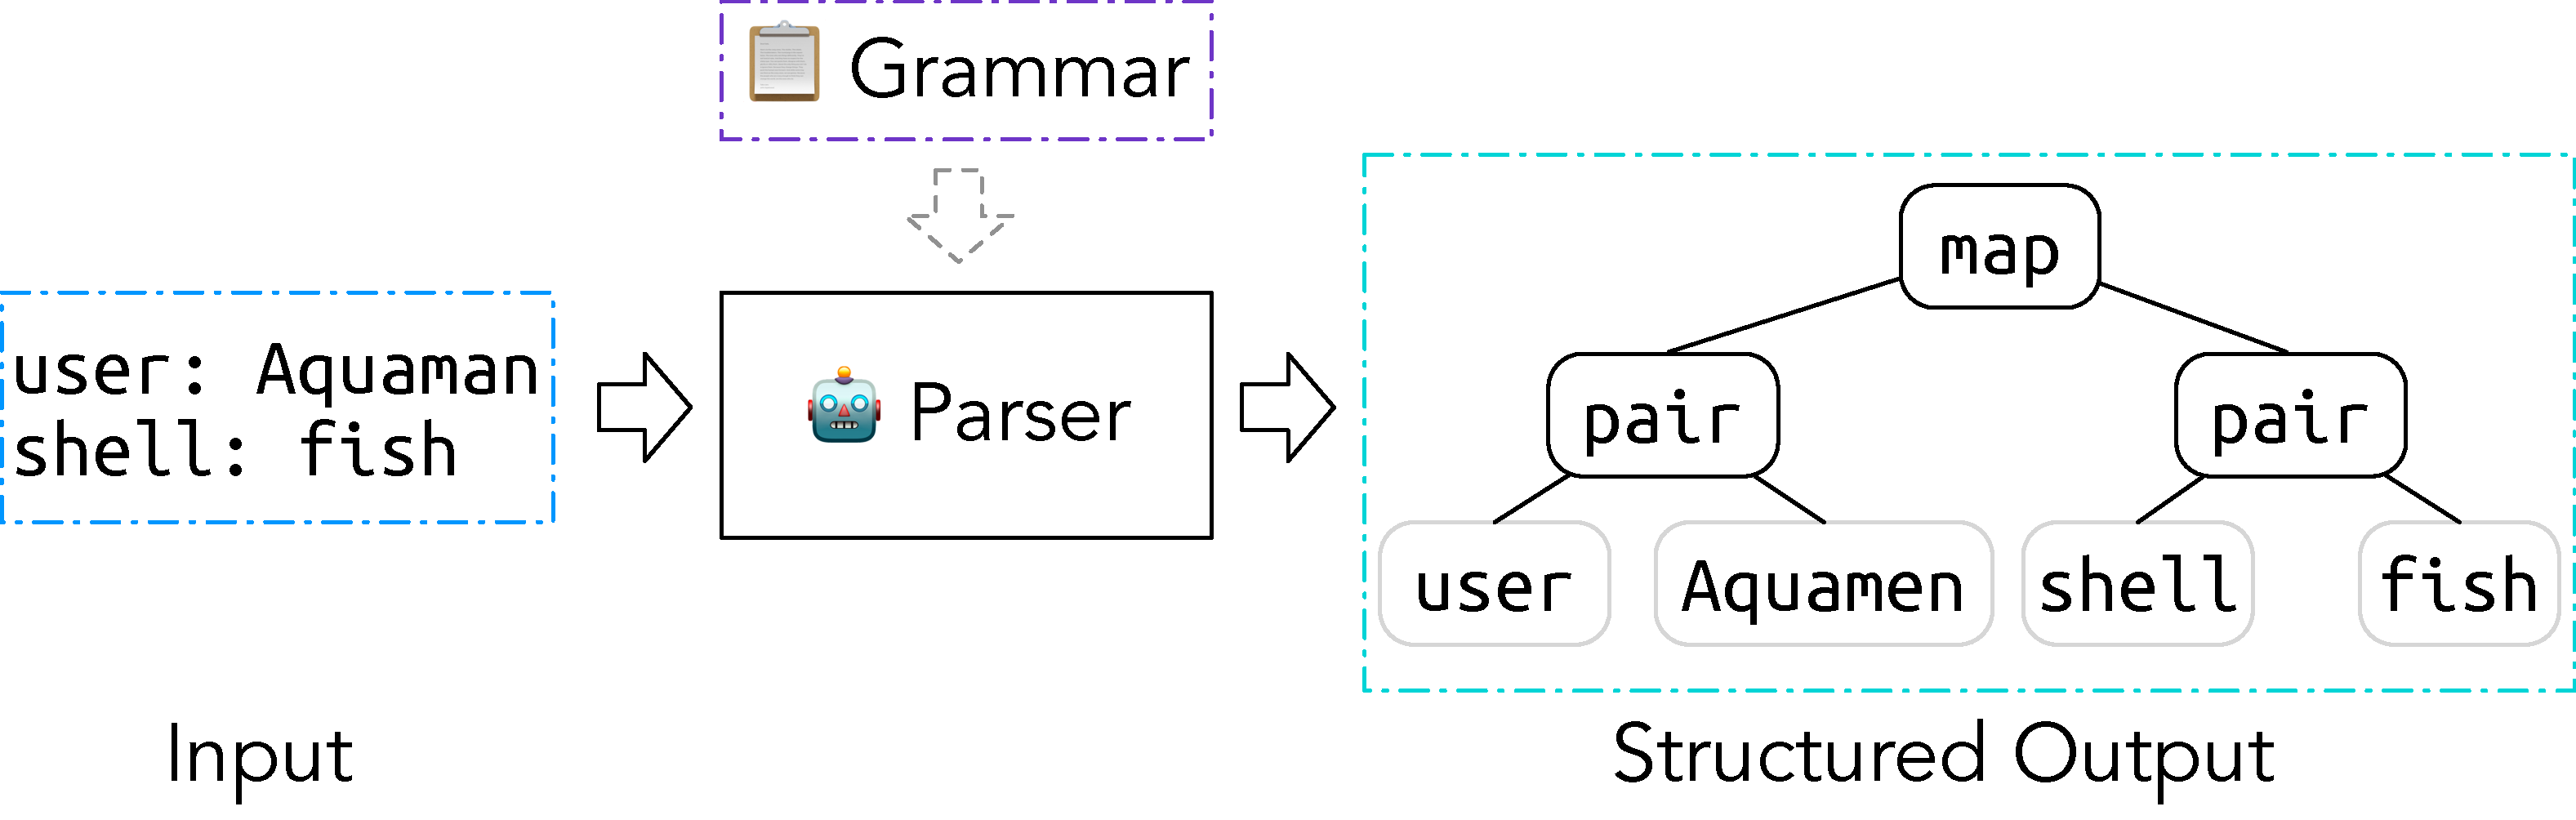
\includegraphics[width=.8\textwidth]{Parsing}
  \caption{Simplified view of the parsing process}
\end{figure}

This thesis concerns itself with the parsing process of languages that are able to express configuration data (e.g. INI, TOML, \glstext{YAML}). These languages form an interesting subpart of formal languages, since accessing key-value based persistent configuration data is a common task for many computer programs.

Just like people disagree about the “best” configuration format, there is currently no consensus, as to which is the ideal way to parse configuration data. There are many possible ways to parse and store data. Notable examples include:

\begin{itemize}
  \item bidirectional programming~\cite{foster2005combinators, bohannon2006relational, lutterkort2008augeas, ko2016bigul, raab2016improving},
  \item code produced by a parser generator~\cite{denny2008ielr, parr2014adaptive, warth2016modular, bates2017aprt},
  \item Serialization libraries~\cite{sumaray2012cds, pacini2015performance}, and
  \item Hand-written parsers~\cite{myers2008cparser, bendersky2012clang}
\end{itemize}

. Currently the possibilities to compare different parsing techniques are limited. The naive approach would be to just run different parsers on the same data. In practice however, this approach is not usable, since parser tools tend to produce very different data structures. Some of them do not produce data structures at all, instead they let the user specify subroutines that should be called when the parser matches parts of the grammar.

As part of this thesis we will tackle this problem, using different parsing techniques within a common configuration framework. This integration eliminates the problem of comparing the parsing process under different circumstances, since the data structures the parsers create will always be the same. We will use \href{http://web.libelektra.org}{Elektra}, a key-value database, as configuration framework. Elektra’s storage plugin interface will act as foundation for the parsing process. In the end the thesis should provide answers about which parsing techniques provide an ideal balance between performance and usability.

\section{Aim of the Work}
\label{sec:aim_of_the_work}

Elektra~\cite{raab2010modular, raab2017context} is a plugin based framework that stores configuration parameters in a \gls{KDB}. Elektra reads and stores configuration data via so-called \emph{storage plugins}.

\begin{figure}[H]
  \centering
    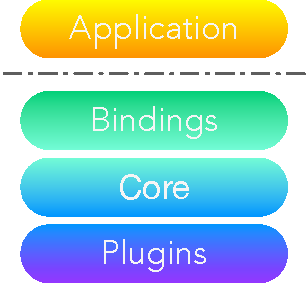
\includegraphics[width=.3\textwidth]{Elektra}
  \caption{Architecture diagram of Elektra}
\end{figure}

As part of this thesis we compare various ways of parsing. For that purpose we wrote and generated parsing code for different storage plugins. All of these storage plugins parse a minimal subset of \glstext{YAML}, a human readable configuration language. We looked at the following parsing technologies:

\begin{itemize}
  \item handwritten parser (recursive descent),
  \item \glstext{ALL(*)} parser generator (\href{http://www.antlr.org}{ANTLR}),
  \item LR parser generator (\href{https://www.gnu.org/software/bison}{Bison}),
  \item Earley parser (\href{https://github.com/vnmakarov/yaep}{YAEP}),
  \item \glstext{PEG} parser (\href{https://github.com/taocpp/PEGTL}{PEGTL}),
  \item parser combinator (\href{https://github.com/orangeduck/mpc}{mpc}), and
  \item bidirectional programming (\href{http://augeas.net}{Augeas})
\end{itemize}

. We compare the parsing code according to the following criteria:

\begin{itemize}
  \item runtime performance,
  \item memory usage,
  \item code size,
  \item overall code complexity,
  \item ease of extensibility and composability, and
  \item error reporting
\end{itemize}

. In the scope of the above comparison we answer the questions below.

\begin{restatable}{question}{speed}
  \label{que:speed}
  How does the theoretic runtime complexity of the parsing methods compare to the actual measured runtime of the parsing code?
\end{restatable}

\begin{restatable}{question}{closeness}
  \label{que:closeness}
  Which parsing technique allows us to stay closest to the definition of the configuration language? Does staying close to the given definition,
  allow us to extend and improve the parser and its support code more easily?
\end{restatable}

\section{Methodological Approach}

The methodological approach for this thesis consists of the steps below.

\begin{description}[style=multiline, leftmargin=3.2cm, font=\bfseries]

  \item[Literature Review] We determined the current status of parsing techniques suitable for configuration file parsing. We then chose appropriate libraries for the parsing techniques listed in the section “\nameref{sec:aim_of_the_work}”.

  \item[Discussion] To determine a minimal usable subset of \glstext{YAML} we discussed common features required for a new Elektra storage plugin with some of the current developers as part of an presentation and subsequent discussion.

  \item[Implementation] We wrote parsing code that handles our minimal \glstext{YAML} subset. In this phase we also added other necessary support code to Elektra.

  \item[Comparison] As noted in “\nameref{sec:aim_of_the_work}” we evaluated the different implementations of our minimal \glstext{YAML} subset parsers.

  \begin{description}
    \item[Runtime Benchmark] For the runtime comparison we use benchmarks to determine the speed of the different parsing code. In this part of the thesis, we answer \Cref{que:speed}.

    \item[Memory Profiling] For the memory comparison we use a memory profiling tool to determine the heap memory usage of the \glstext{YAML} plugins.

    \item[Code Count] We counted the number of code lines with a code line counting tool. This method allow us to consider only actual code, ignoring blank lines and comments.

    \item[Complexity Measurement] We measured the \gls{CC} of the code using a static analyzer.

    \item[Extensibility \& Composability Check] To analyze the extensibility and composability of the parsing code we looked at the code difference of commits for certain features and bug fixes. We counted the amount of updated code lines to determine the extension effort. This measurement, together with a comparison between the grammar specification of \glstext{YAML} and the code created in this thesis, will help us to determine the answer for \Cref{que:closeness}.

    \item[Error Reporting] To determine the quality of the error messages we created erroneous files and compared the quality of the resulting error output.
  \end{description}

\end{description}

\chapter{Background}

In the first part of the thesis we look at the current state of parsing according to the literature. After that we provide a short overview of Elektra, the key-value storage framework we use in the thesis.

\section{State of the Art}
\label{sec:state_of_the_art}

\subsection{Parsing}
\label{sec:parsing}

The book \citetitle{grune2008parsing}~\cite{grune2008parsing} provides a good overview of various up-to-date parsing algorithms. It covers the most popular techniques and also less well known methods up to 2006. The book also describes various classification possibilities for parsing techniques \cite[p. 85]{grune2008parsing}. The most common classification is the division into bottom-up and top-down parsers.

\begin{figure}
  \centering
  \begin{subfigure}[t]{.48\textwidth}
    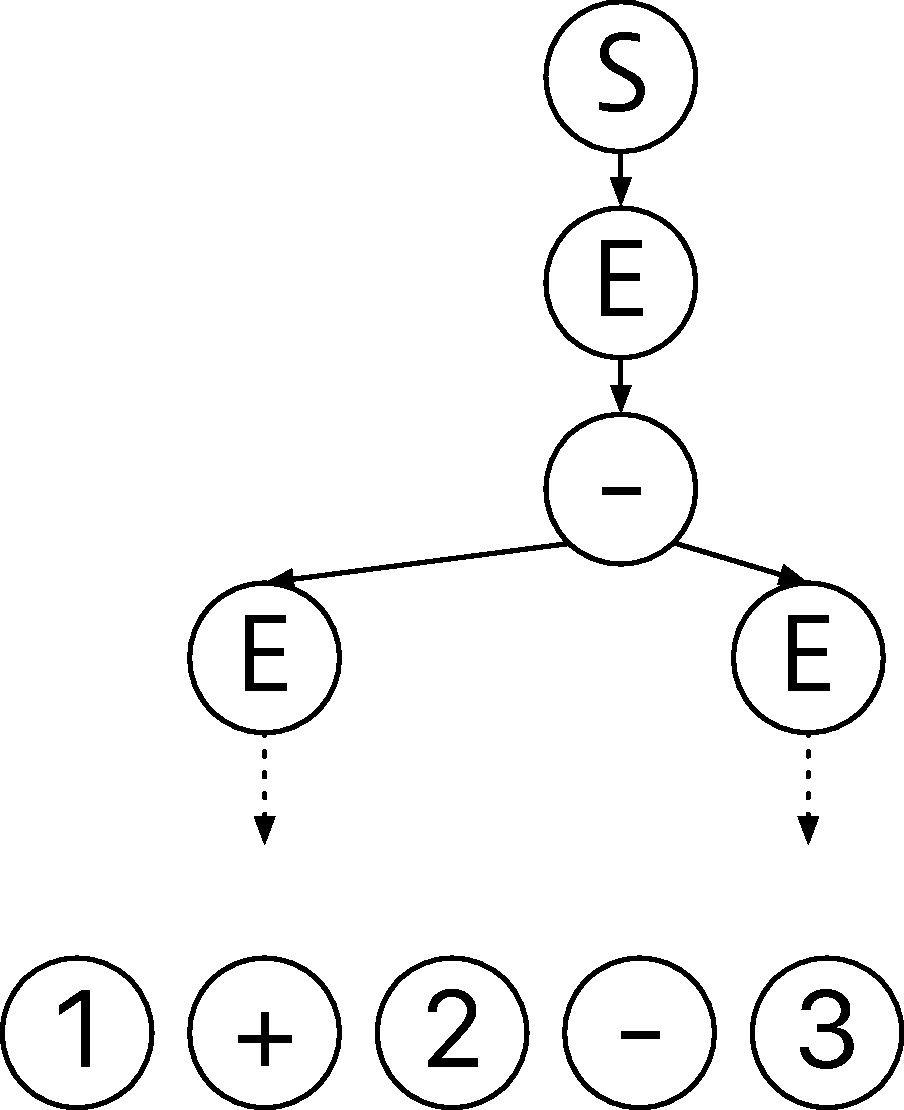
\includegraphics[width=\linewidth]{Top-Down}
    \caption{A top-down parser predicts and matches rules from the start symbol downwards.}
  \end{subfigure}
  \quad
  \begin{subfigure}[t]{.48\textwidth}
    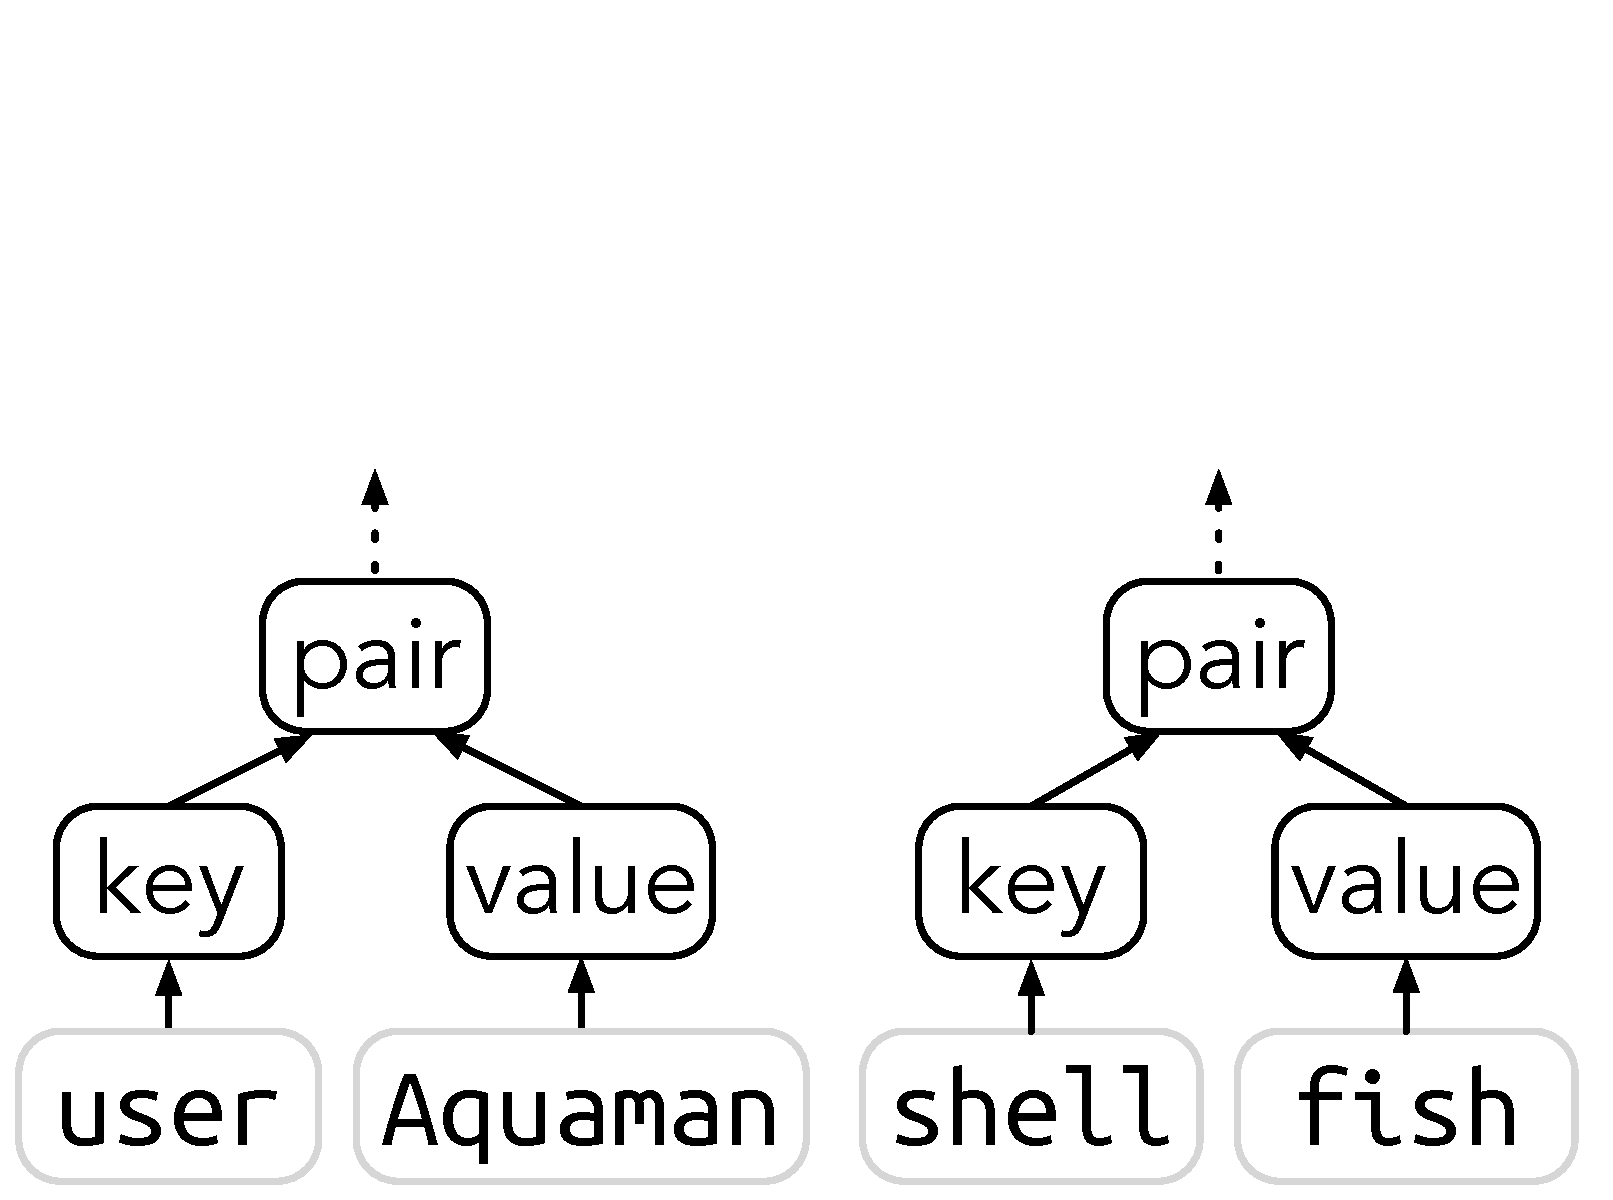
\includegraphics[width=\linewidth]{Bottom-Up}
    \caption{A bottom-up parser recognizes text starting with the terminal symbols.}
  \end{subfigure}
  \caption{Matching in top-down and bottom-up parsers}
\end{figure}

In \emph{top-down parsing} the parser starts with a hypothesis about the structure of the given data. The parser then tries to predict and match parts of the structure, starting from larger parts working its way down to smaller elements.

We can further categorize parsing into \emph{directional} and \emph{non-directional} methods. Directional methods read the input from left to right, while non-directional methods can use an arbitrary order. This implies that directional methods are simpler and faster, but less powerful, than their non-directional counterparts. As part of this thesis we only consider directional methods, since they are faster and powerful enough to parse configuration data.

One of the most popular directional top-down methods is \emph{\glstext{LL} parsing}. While this technique is quite old – \citetitle{grune2008parsing} (p. 584) mentions a paper from 1961 belonging to the \glstext{LL} category – it is still actively used and researched. The basic idea behind \glstext{LL} parsing is simple: Begin with the start symbol of the grammar and the first character of the text. Then predict the next grammar rule, looking at the text to the right of the current position. We can categorize the technique further according to the number of characters/tokens the parser uses to predict the next rule. If the parser uses one token of look-ahead we speak of an \glstext{LL}(1) parser, if it uses k tokens of lookahead we speak of an \glstext{LL}(k) parser~\cite{rosenkrantz1969properties}.

Two common methods to create an \glstext{LL} parser are:

\begin{enumerate}

  \item Implement the parser code using a set of mutually recursive procedures (recursive descent parser). The code for this is either written by hand or produced by a parser generator such as \GlsShort{ANTLR}~\cite{parr2013recursive}.

  \item Use a parser generator to create a table-based parser.

\end{enumerate}

Examples of popular active projects that use a handwritten recursive descent parser include \href{http://clang.llvm.org}{clang}~\cite{bendersky2012clang} and \href{http://gcc.gnu.org}{GCC}~\cite{myers2008cparser}. The \href{http://www.antlr.org/about.html}{about page} for \gls{ANTLR} mentions some projects that use its generated recursive descent parsers. The list includes Twitter, wich uses ANTLR for query parsing and parsers for the languages used in the Apache Hadoop projects Hive and Pig~\cite{parr2013definitive}.

Some of the latest research developments in \glstext{LL} parsing include \glstext{LL}(*) parsing~\cite{parr2011ll} and its successor \gls{ALL(*)}~\cite{parr2014adaptive}. Both of these algorithms use dynamic lookahead~\cite[p. 1]{parr2011ll}. While \glstext{LL}(*) parsing uses a static algorithm for rule prediction, ALL(*) analyzes the input at runtime to improve prediction. As consequence of this parsers that use the \gls{ALL(*)} algorithm will be faster after an initial warm-up phase~\cite[p. 3]{parr2014adaptive}. LL(*) is part of \gls{ANTLR}~3~\cite[p. 3]{parr2014adaptive}, while \gls{ANTLR}~4 uses Adaptive \glstext{LL} parsing.

As we already mentioned before, the other popular parsing technique besides top-down-parsing is \emph{bottom-up parsing}. In bottom-up parsing the parser builds a structure starting with the smallest elements of the grammar (terminals). The parser then combines these elements into larger parts. One of the earliest entries in the \emph{linear bottom-up} parser category is the \glstext{LR}(k) parser~\cite{knuth1965translation}. Just like in \glstext{LL}(k) parsing, k specifies the number of lookahead symbols the parser uses.

\begin{sloppypar}
Unlike \glstext{LL} parsers, \glstext{LR} parsers are usually not created by hand, but generated by a parsing tool such as \href{https://www.gnu.org/software/bison}{Bison} or \href{http://dinosaur.compilertools.net/yacc}{Yacc}. Since \glstext{LR}(k) tables are very large, even for a small numbers of k, the parser tools mentioned before usually generate less powerful but smaller and faster LALR(k)~\cite{deremer1969practical} parsers.
\end{sloppypar}

\glstext{LR}(k) parsers are able to handle more grammars than \glstext{LL}(k) parsers for the same constant k~\cite[section “Lookahead”]{haberman2013ll}. However, \glstext{LR} parsers are still not able to handle ambiguous grammars. For this purpose \citeauthor{lang1974deterministic} describes the Generalized \glstext{LR} (GLR)~\cite{lang1974deterministic} method that is also able to process these types of grammars. GLR parser are sometimes also called Tomita parsers~\cite{tomita1985efficient} after the author that described the first implementation of a generalized \glstext{LR} parser.

Recent research in the space of directional bottom-up parsing includes improved versions of techniques that are almost as powerful as canonical \glstext{LR}(1). One of the most promising methods is IELR(1)~\cite{denny2008ielr}. The advantage of IELR(1) over LALR(1) is that it handles conflict resolution better. Parser tools such as Bison use conflict resolution to handle non-\glstext{LR} grammars, i.e. grammars that contain rules where the parser is not able to decide what to do next. To handle these types of conflicts the grammar designer manually specifies which decision the parser should take. The current version of the parsing tool Bison supports an experimental version of IELR(1).

Most parsing techniques can be categorized as either top-down or bottom-up. However, some techniques use a combination of both approaches. Others are usually not listed under one of the label top-down or bottom up, because they provide other features that the designer of these parsers deem more important, or they use features that do not fit well within either of these groups. In the remainder of this section we will discuss some of these techniques.

A method that can be categorized as either top-down technique with bottom-up recognition, or bottom-up technique with a top-down component~\cite[p. 206]{grune2008parsing} is \emph{Earley Parsing}~\cite{earley1970efficient}. Earley parsing is able to handle any context free grammar. This means the technique is as powerful as GLR parsing. This advantage comes at the cost of runtime. While \glstext{LL} parsing and \glstext{LR} parsing run in linear time depending on the length of the input ($O(n)$), Earley Parsing has an upper boundary of $O(n³)$. However, in \citeyear{leo1991general} \citeauthor{leo1991general} showed that an improved version of the algorithm handles most \glstext{LR}(k) grammars in linear time~\cite{kegler2011marpa, leo1991general}. In \citeyear{aycock2002practical} \citeauthor{aycock2002practical} described improvements to the algorithm~\cite{aycock2002practical}. Their version of Earley Parsing boosts the runtime in cases where the grammar contains nullable (empty) grammar rules. Recently \citeauthor{kegler2011marpa} incorporated the changes proposed by \citeauthor{leo1991general}, \citeauthor{aycock2002practical} in \href{http://savage.net.au/Marpa.html}{Marpa}~\cite{kegler2011marpa}.

\begin{figure}
  \centering
    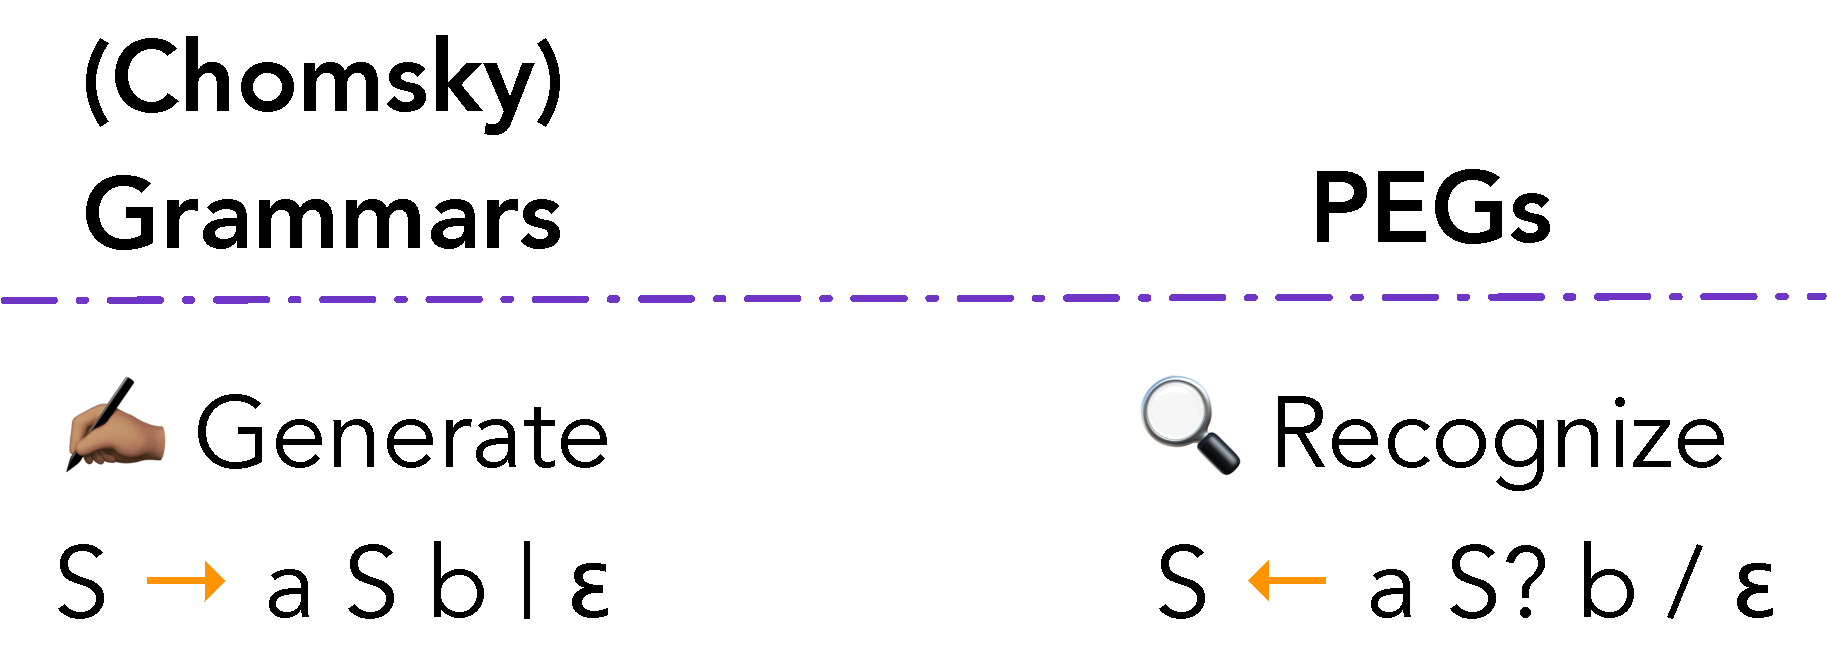
\includegraphics[width=0.45\textwidth]{Chomsky-PEGs}
  \caption{Both the Chomsky grammar on the left and the PEG on the right describe the same language $ \{ aⁿ bⁿ | n ≥ 0 \} $.}
\end{figure}

All the methods we mentioned until now work with a description that is based on a (context-free) Chomsky grammar. These grammars describe a way to \emph{generate} words and sentences of a given language. Another way to specify the structure of a language is to give a description on how to \emph{recognize}~\cite[p. 506]{grune2008parsing} the words and sentences of a language. One popular recognition system are \glspl{PEG}. They were introduced by \citeauthor{ford2004parsing} in the paper \citetitle{ford2004parsing}~\cite{ford2004parsing}. \citeauthor{ford2002packrat} also describes how to write an efficient (top-down) parser that handles these types of grammars in linear time~\cite{ford2002packrat}. This method, called Packrat parsing, uses a specialized version of memoziation~\cite[p. 1]{ford2002packrat} to save intermediate results of the parsing process. We should mention that it is generally not clear, if memoization provides a runtime performance advantage in practice for a certain grammar. In the article~\citetitle{hudak2008dcgs}~\cite{hudak2008dcgs} \citeauthor{hudak2008dcgs} show that not using memoization can decrease the actual runtime of a PEG parser.

Just like Packrat parsing, \emph{combinatory parsing}~\cite{frost1992constructing, hutton1992higher} specifies a method to create recursive descent parsers. As the name suggests, the focus in combinatory parsing is the composability of parsers. The technique is usually used in functional programming languages, such as Haskell. These languages support higher order functions, i.e. functions that take other functions as their parameters~\cite[p. 564]{grune2008parsing}. In combinatory parsing the parser creator typically starts by specifying parsers (functions) for the simplest parts of the grammar (terminals). She or he then goes on to combine these simpler parsers into more powerful parsers for more complex rules (non-terminals). Combinatory parsing has similar problems as other top-down techniques such as \glstext{LL} parsing. One of these problems are left recursive grammar rules, i.e. rules that include references to themselves in the leftmost part of the right-hand side. Recently \citeauthor{frost2007modular} described a method to handle left recursive rules in combinatory parsing efficiently in the article \citetitle{frost2007modular}~\cite{frost2007modular}.

A method that is not a parsing technique per se, but a way to specify conversions of data from a source structure to a target structure and back is \emph{bidirectional programming}~\cite{foster2005combinators, bohannon2006relational}. The specification that allows this conversion is called a lens~\cite{foster2005combinators}.

\begin{figure}[H]
  \centering
    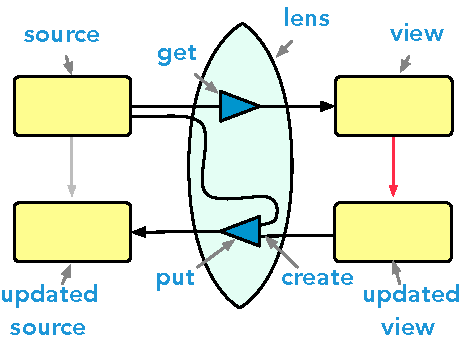
\includegraphics[width=.4\textwidth]{Lens}
  \caption{Lenses provide a way to both parse (get) and write (put) structured data \newline (Source: \href{http://www.seas.upenn.edu/~harmony/manual.pdf}{Boomerang Programmer’s Manual})}
\end{figure}

A programming language used to specify such lenses is Boomerang~\cite{bohannon2008boomerang}. The research of the Boomerang project lead to the creation of another project that uses lenses to parse configuration data: \href{http://augeas.net}{Augeas}. Augeas converts configuration data into a tree like representation. \citeauthor{berlakovich2016universal} implemented an Augeas plugin for Elektra as part of his Bachelor thesis~\cite{berlakovich2016universal}.

\subsection{Configuration File Parsing}
\label{sec:configuration_file_parsing}

The literature overview in the previous section focused on parsing in general. It is know time to take a look at the current state of configuration file parsing and how it differs from the well know problem of parsing (general purpose) programming languages.

There exists extensive literature about parsing of programming languages and compiler design. The topic is even part of famous computer science books such as \citetitle{ullman1977principles}~\cite{ullman1977principles} and \citetitle{aho2006compilers}~\cite{aho2006compilers}, commonly also know as “Dragon” books~\cite{parr2009language}, named after the Dragon (waiting to be slain) on their covers.

While parsing and compiling computer languages is seen as “slaying a Dragon”, configuration file parsing is arguably a much simpler task. The reason for this is that the purpose of configuration languages, usually only specifying data, is a subset of the purpose of programming language, which also manipulate data. This superset feature of programming language makes them sometimes also interesting for the purpose of storing configuration data~\cite{balmer2013lua}. Since configuration data is used by many programs that usually do not ship with, or require an interpreter or compiler, most configuration files do not use the syntax of a general purpose programming language. These “data only” configuration file formats can be classified roughly into three categories.

\begin{description}
  \item[Custom configuration file formats] specify data for a specific application. Examples are the \href{https://en.wikipedia.org/wiki/Fstab}{\code{fstab}} file used by the Unix program \sh{mount}, or the \href{https://en.wikipedia.org/wiki/https://en.wikipedia.org/wiki/Hosts_file}{\code{hosts}} file used for name resolution.

  \item[General purpose configuration formats] such as \href{https://en.wikipedia.org/wiki/INI_file}{INI}, and the \href{https://en.wikipedia.org/wiki/Property_list}{Property list} file format are used mainly to store configuration data of many different applications.

  \item[Serialization formats] such as \gls{JSON}, \gls{YAML}, and \gls{XML}, store all kinds of data, not only limited to configuration purposes.
\end{description}

\begin{figure}[H]
  \centering
  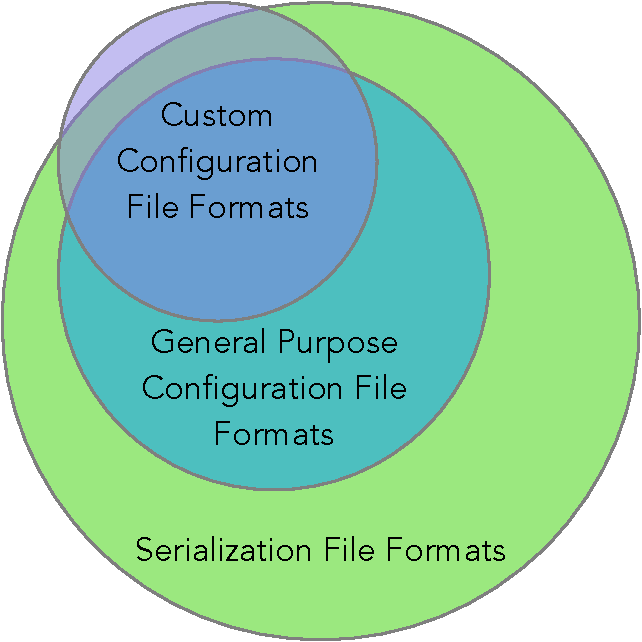
\includegraphics[width=.45\textwidth]{ConfigurationFileFormats}
  \caption{The Venn diagramm above shows an overview of the overall expressiveness of the formats usually used for configuration data. Please note, that the size of the circles \emph{does not} show the level of expressiveness of a certain category of file formats, i.e. a circle twice as large does not represent twice the level of expressiveness.}
\end{figure}

In general we can use serialization formats, to specify the same data as we can using general purpose configuration languages. For example, in macOS Property lists can be stored using \glstext{JSON} or \glstext{XML} on disk. The same is not true for custom configuration formats, which are often very simple, but can sometimes also use programming language code. Popular examples for this are the configuration files of shells, such as \code{bash}, \code{fish} and \code{zsh}. These shells use the same syntax for programming and configuration data.

We already said that most configuration file formats do not use the syntax of general purpose programming languages, but rather syntax only able to specify and \emph{not} to modify data. The simplicity of some of these languages often means that parsing code for them is not written by an expert. Especially for simple custom configuration file formats, the same person that implements a program often also implements the parser for its configuration file format. This can result in configuration code that integrates tightly into a program, decreasing the extensibility of the application. Other problems of parsers not written by experts include: bad or no error message support, no support for error recovery, and insufficient support for different file format encodings.

Some of these problems can be solved using a configuration file library that is available for most of the more popular general file formats. Such a library takes care of the parsing, loosening the integration of an application and its configuration code. Some problems of theses libraries are that they

\begin{itemize}
  \item often do not consider order, and
  \item almost always throw away comments
\end{itemize}

when they write back data into a configuration file. This is a problems, since for example, comments in configuration files can be very helpful in averting misconfiguration.

A configuration library that keeps the order of entries and comments intact is Augeas~\cite{lutterkort2008augeas, berlakovich2016universal}. As we already wrote in the previous section Augeas uses so-called lenses to both parse and write back configuration. The problem of lenses is that they only support regular languages~\cite{chomsky1959certain} properly. For example, as we found out during the development of the parsing code for the thesis, the \href{https://github.com/hercules-team/augeas/blob/d555a995a06ac81cab62d016d6eaff8a7ba64a2e/lenses/yaml.aug}{YAML lens} of Augeas only supports mapping data with a nesting level of two.

Compared to Augeas, Elektra~\cite{raab2010modular, raab2017context}, with its plugin based parsing system also supports context free and even context sensitive configuration languages. This is the case, since Elektra can use a general purpose programming language to parse code. Using metadata Elektra is also able to store the content of comments and keep the order of configuration data intact, when writing data back. The code for this has to be implemented in the plugin itself, which can become problematic. For example, while Elektra’s \href{https://github.com/ElektraInitiative/libelektra/tree/3e6e0254a54d3ad9642091550ce9c560d8cf38dd/src/plugins/ini}{INI plugin} preserves comments and the order of entries, its code is also quite complicated and error-prone. As we already stated in “\nameref{sec:aim_of_the_work}” we want to improve this situation using state of the art parsing techniques for our YAML subset plugins.

\subsection{Error Handling}
\label{sec:error_handling}

The usual goal in parsing is the processing of grammatically correct input. However, since editing configuration data is often done by hand, there is always a possibility of erroneous input. A method to inform the user about such errors is essential. As pointed out by Terence \citeauthor{parr2013definitive} in \citetitle{parr2013definitive}~\cite[p. 151]{parr2013definitive} we also need to inform the user about the reason for an error:

\begin{quote}
  In other words, a parser that responds with “Eh?” and bails out upon the first syntax error isn’t very useful for us during development or for our users during deployment.
\end{quote}

The process of reacting to errors is called \emph{error handling}. Error handling can be grouped into four dependent stages~\cite{ruefenacht2016error, pottier2016reachability}:

\begin{enumerate}
  \item error detection,
  \item error diagnosis,
  \item error recovery, and
  \item error correction
\end{enumerate}

. We are mainly interested in the first three items, since error correction is generally not possible without the possibility of fixing errors incorrectly.

\emph{Error reporting} is the results of

\begin{itemize}
  \item detecting that input is incorrect (error detection),
  \item finding what part of the input was incorrect (error diagnosis), and
  \item trying to resume the parsing process in case of errors (error recovery).
\end{itemize}

The current state of error reporting capabilities depend strongly on the parsing technique.

In general, top-down recursive descent parsers \emph{without backtracking}, especially those written by hand, are able to produce good error messages. The reason for this is that such parsers have information about the higher level grammar rules that matched until the error point. While the error messages produced by recursive descent parsers can be good, writing error logic by hand makes the code more complicated. If we want to react to multiple errors in a configuration file we also need to implement error recovery, which can be “tedious and easy to screw up”~\cite[p. 160]{parr2013definitive}. \glstext{ANTLR} produces parsers that integrate techniques such as token deletion, token insertion, and resynchronization to produce parsers that provide “a good error reporting facility and a sophisticated error recovery strategy for free” according to its main author~\cite{parr2013definitive}.

Bottom up parsers, produced by a tool such as Bison are not suited to provide good error messages~\cite{jeffery2003generating}. Error recovery in Bison produced parsers even requires changes to the grammar~\cite{donnelly2019bison}. There exists promising research work to improve the current situation. In \citetitle{jeffery2003generating}~\cite{jeffery2003generating}  \citeauthor{jeffery2003generating} shows how his tool merr can help a user to specify error messages based on example input in a C based parser produced by \glstext{Yacc} or Bison. \citeauthor{jeffery2003generating}’s semi-automated approach is based on error states of the parser and improves on the previous technique used in the Icon programming language, where developers manually modified the source code produced by a custom version of \glstext{Yacc}. Since  \citeauthor{jeffery2003generating}’s work looks promising, another similar approach was also used in the old Bison parser\footnote{The developers of Go switched to a hand-written parser written in Go in 2016~\cite{pike2017reddit, go2016release}.} for the programming language Go~\cite{cox2010errors}. Recently \citeauthor{pottier2016reachability}~\cite{pottier2016reachability} extended \citeauthor{jeffery2003generating}’s work and added example based error reporting in the \glstext{LR} parsers of the CompCert C compiler~\cite{kaestner2018compcert}. In \citetitle{pottier2016reachability} \citeauthor{pottier2016reachability}~\cite{pottier2016reachability} writes that he thinks that “the quality of CompCert’s diagnostic messages is now on par with that of \texttt{clang} and \texttt{gcc}”.

For now we only talked about the error capabilities of deterministic parsers – such as \glstext{LL} and \glstext{LR} parser – i.e. parser that do not back up. These parsers read the input deterministically from left to right. They therefore report the first position, where the parsed input is not part of the language described by the grammar anymore. This behavior is also known as (longest) correct/viable prefix property~\cite{sippu1990parsing, ruefenacht2016error, maidl2016labeled, pottier2016reachability}. Parsers with backtracking, such as recursive descent parsers \emph{with backtracking}, \glstext{PEG} parsers and the closely related combinatory parsers usually do not have this property. While backtracking makes these parsers more powerful, the quality of error messages suffer. The problem is that backtracking can occur both because of a valid choice in the grammar or because of an error in the input.

There has been research to improve the situation, especially in \glstext{PEG} parsers. In his master thesis~\cite{ford2002packrat} \citeauthor{ford2002packrat} already describes one option to produce meaningful error messages. His parser records all parsing results and uses the one that matched the farthest to the right in the input for error messages. In \citetitle{maidl2016labeled}~\cite{maidl2016labeled} \citeauthor{maidl2016labeled} show that this error strategy can also be added to every \glstext{PEG} library that supports semantic actions. They also introduce a form of error reporting, inspired by the excepting handling mechanism of programming languages, based on grammar annotations called labeled failures~\cite{maidl2016labeled}.

\section{Elektra}

In this section we describe some of the concepts of Elektra, the software that provides the common storage facility for our \glstext{YAML} parsers, further. Elektra is a framework that stores data in a \emph{global hierarchical key-value database}.

\subsection{\cc{Key}}

The most basic entity in Elektra is the \cc{Key} structure. A concrete instance of a \cc{Key} contains at least one non-empty attribute, which is the \emph{name} of the \cc{Key}. In the remainder of the thesis we will also often use the term \emph{key} - please notice the non-gray background – to refer to the name of a \cc{Key}.

\begin{figure}
  \centering
    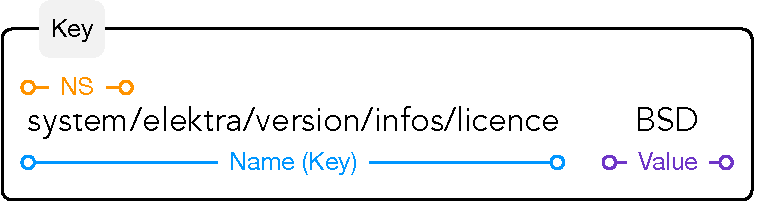
\includegraphics[width=.6\textwidth]{Key.pdf}
  \caption{In Elektra a \cc{Key} stores a single \textcolor{Aqua}{key}-\textcolor{Purple3}{value} pair. The first part of the name specifies the \textcolor{orange}{namespace} (NS).}
  \label{fig:key}
\end{figure}

Besides the name an instance of a \cc{Key} usually also stores a value. Figure~\ref{fig:key} shows an example \cc{Key} with the \textcolor{Aqua}{name} \code{system/elektra/version/infos/licence} and the \textcolor{Purple3}{value} \code{BSD}.

Since Elektra stores data in a hierarchical database, a key consists of parts – separated by \code{/} – that determine the location in the database. The key in Figure~\ref{fig:key} consists of 5 parts. The first part \code{system} is the \textcolor{orange}{namespace} (NS) of the key. Elektra uses namespaces to specify context dependent data. For example, user specific data is stored under the namespace \code{user}. Elektra uses 5 namespaces to separate data:

\begin{itemize}[style=multiline, leftmargin=1.8cm]
  \item [\code{system}] specifies data values for the whole system,
  \item [\code{user}] contains data for the current user,
  \item [\code{dir}] stores data for the current directory,
  \item [\code{spec}] contains specification of other keys, and
  \item [\code{proc}] stores in-memory data
\end{itemize}

. We can use a so-called \emph{cascading} key to select the most appropriate namespace. A cascading key does not start with a namespace but rather with a leading slash. Let us look at an example. We assume our database contains the keys:

\begin{itemize}
  \item \code{system/key}, and
  \item \code{user/key}
\end{itemize}

. If a non-superuser requests the cascading key \code{/key}, then Elektra will select \code{user/key}. If the database also contains a key \code{dir/key} for the current working directory, then Elektra will select this key instead.

\subsection{\cc{KeySet}}
\label{sec:keyset}

As we already saw in the example before, usually we store not only one, but multiple key-value pairs in the database. For this purpose Elektra provides the structure \cc{KeySet}. A \cc{KeySet} contains a set of \cc{Key} objects. The name of each \cc{Key} has to be different. If we add a new \cc{Key} with an already existing name to the \cc{KeySet}, then Elektra will just overwrite the old \cc{Key} with the same name.

\begin{figure}
  \centering
    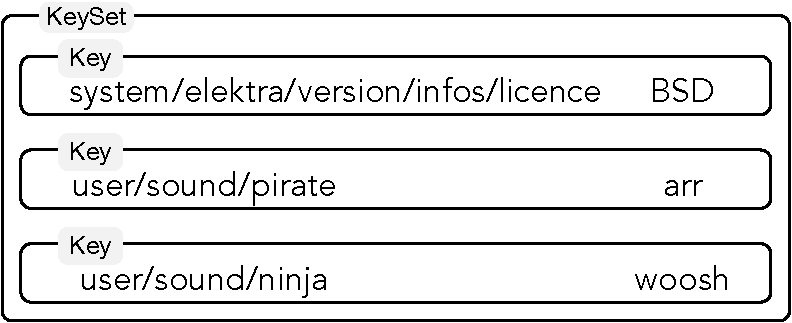
\includegraphics[width=.6\textwidth]{KeySet}
  \caption{Elektra uses \cc{KeySet} structures to save multiple key-value pairs}
  \label{fig:keyset}
\end{figure}

A \cc{KeySet} allows us to structure data in a fashion similar to a map (a.k.a. hash, map, hashmap, dictionary). Maps are an important data structure, especially in high level programming languages like \href{https://www.python.org}{Python} or \href{https://www.ruby-lang.org}{Ruby}. Let us look at an example. We take the last three \cc{Key} objects in Figure~\ref{fig:keyset}, remove the namespace and translate the data to a Python dictionary:

\begin{pythoncode}
  sound = {'pirate': 'arr', 'ninja': 'woosh'}
\end{pythoncode}

. We see that a value in a \cc{KeySet} also maps to a value in the dictionary, while the last part of the key (name) maps to the key in the dictionary.

Apart from the map, another important data structure is the array. Elektra also supports arrays. For that purpose Elektra adds the character \code{\#}, and the index to array elements. For example, the following Python list:

\begin{pythoncode}
  characters = ['pirate', 'ninja']
\end{pythoncode}

would translate to the \code{KeySet} shown in Figure~\ref{fig:array}.

\begin{figure}
  \centering
    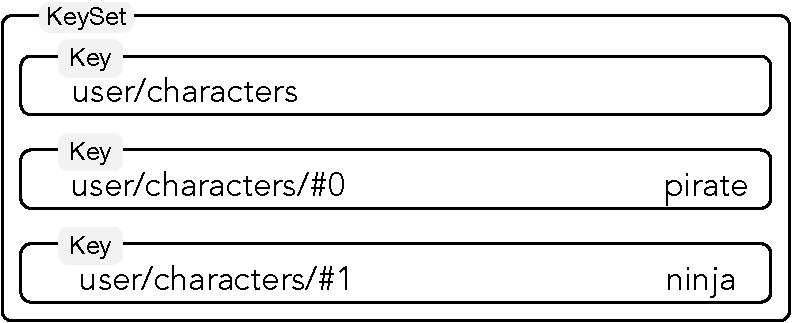
\includegraphics[width=.6\textwidth]{Array}
  \caption{Elektra uses the character \code{\#} to mark array elements}
  \label{fig:array}
\end{figure}

Since Elektra orders a \code{KeySet} alphabetically a \cc{Key} with name \code{\#10} would appear before a \cc{Key} with name \code{\#2}. To fix that problem Elektra adds underscores to keys with larger indizes. For example, the 11th element of an array ends with the name \code{\#\_10}.

One important difference between Python’s list type and Elektra’s array type is that arrays do not need to be continuous. For example, it is possible for an Elektra array to only contain elements with the names \code{\#1} and \code{\#3}, while \cc{Key} entries with name \code{\#0} and \code{\#2} are missing.

Elektra also uses the \cc{KeySet} structure to add \emph{metadata} to single keys. For this purpose each \cc{Key} may store a \cc{KeySet} containing simple key-value pairs. Figure~\ref{fig:metadata} shows an example \cc{Key} containing two meta keys \code{comment} and \code{check/type}.

\begin{figure}
  \centering
    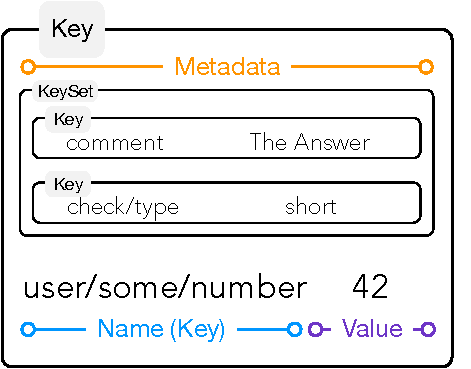
\includegraphics[width=.4\textwidth]{Metadata}
  \caption{Elektra uses a \cc{KeySet} to save metadata for a \cc{Key}.}
  \label{fig:metadata}
\end{figure}

\FloatBarrier
\subsection{Plugins}
\label{sec:plugins}

Apart from basic features, most of Elektra’s functionality is realized as \emph{plugin}. This has the advantage, that Elektra’s core can stay minimal only requiring \href{https://en.wikipedia.org/wiki/C99}{C99}, while plugins are able to implement and use OS specific features.

Many different \href{https://www.libelektra.org/plugins}{plugin categories} exist. Elektra needs at least one resolver and one storage plugin. The resolver plugin handles filenames and replaces files on disk. Storage plugins, on the other hand, parse configuration files and convert read data to a \cc{KeySet}. They are also responsible for writing a modified \cc{KeySet} back to a given file.

In this thesis we are mostly interested in storage plugins. However, we will also use other plugins to implement common functionality for our \glstext{YAML} storage plugins. For this purpose we use the plugin interface of Elektra to pass key sets between plugins.

The order in which Elektra calls a certain plugin is specified via the \emph{contract} of the plugin. For example, a typical storage plugin will use the positions \code{getstorage} and \code{setstorage}. Plugins at the position \code{getstorage} will be called when Elektra tries to read a configuration file, while Elektra calls \code{setstorage} plugins when it is time to write a \cc{KeySet} back to a file. A plugin that wants to further process data will usually use the position \code{postgetstorage} right after \code{getstorage}, and \code{presetstorage} the position before \code{setstorage}.

\begin{figure}
  \centering
    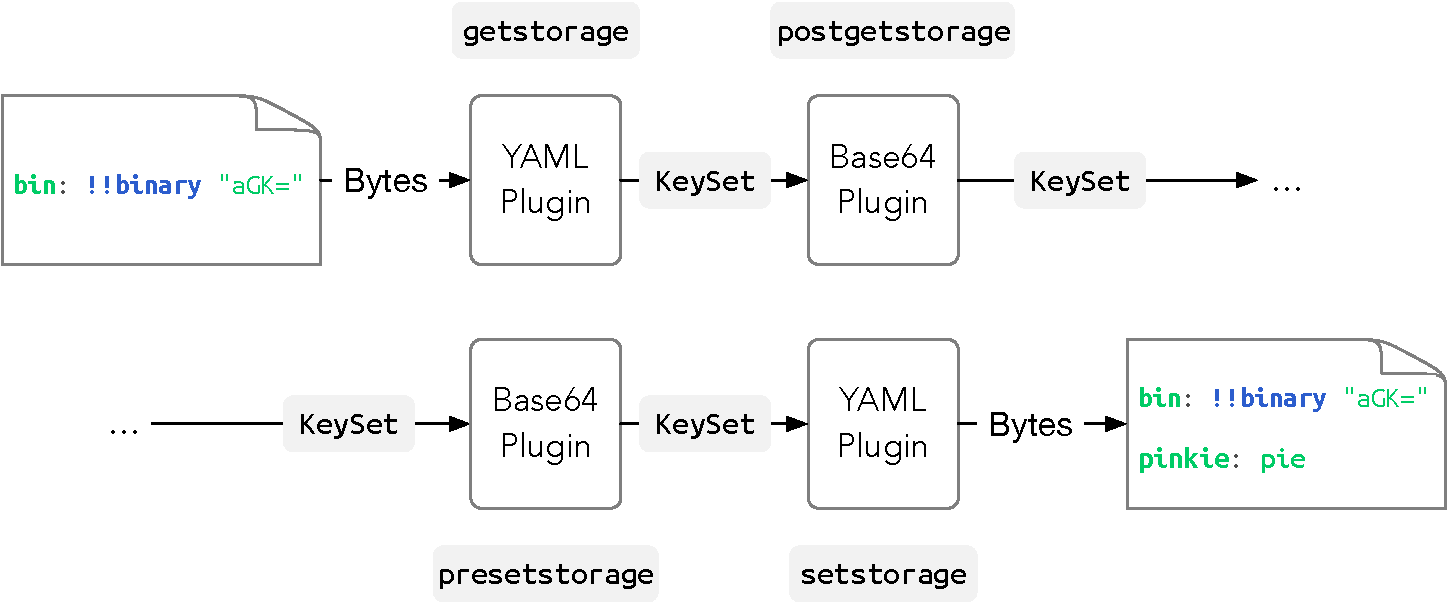
\includegraphics[width=.9\textwidth]{Plugins}
  \caption{Elektra uses multiple plugins to process data.}
  \label{fig:plugins}
\end{figure}

Figure~\ref{fig:plugins} shows a example, where Elektra uses a \glstext{YAML} plugin to read and write data, while a Base64 plugin (see also section “\nameref{sec:base64}”) encodes and decodes binary values. Such a combination of multiple plugins working together is called a \emph{backend}.

In Elektra we \emph{mount} a backend at a certain position of the key-value database. For example, if we mount the backend described above at \code{user/yaml}, then the \glstext{YAML} plugin is responsible for storing and retrieving values below this mountpoint. If we want to save a new \cc{Key} with the name \code{user/yaml/pinkie} and the value \code{pie}, then Elektra

\begin{enumerate}
  \item uses the \glstext{YAML} plugin to convert the current \glstext{YAML} configuration file to a \cc{KeySet},
  \item decodes every binary \cc{Key} with the Base64 plugin,
  \item adds \code{user/yaml/pinkie} to the \cc{KeySet},
  \item encodes every binary \cc{Key} with the Base64 plugin, and
  \item then stores the result to the configuration file using the \glstext{YAML} plugin
\end{enumerate}

.

\section{Related Work}

\subsection{Parser Comparison}

Most of the parser comparison related papers evaluate some form of new parser engine or parser generator against existing parsers or libraries. A recent example of this type of paper is \citetitle{json2019geoff}~\cite{json2019geoff}. In this paper \citeauthor{json2019geoff} use \gls{SIMD} instructions to accelerate the parsing of \gls{JSON} data. In the “Experiments” section of this paper the authors compare their implementation with other JSON parsers, first only using the pure parsing speed, meaning that they ignore the different output of the tested parsers. They also provide a comparison where they show how fast the tested parser are able to find the same data in one of the converted documents from their data set.

While parsing one file format using a specialized parser provides information about how fast we are able to convert certain file formats, this kind of optimization can require substantial manual work. For the plethora of different configuration file formats, it is usually not possible to handcraft parser by hand. Even if it would be possible, some parser need to store information that others do not (e.g. comments), making the process of creating a parser that handles all these tasks by hand even harder. To fix this problem we can generate code for the parser.

There are some papers that compare parser generators themselves. For example, in \citetitle{chen2011full}~\cite{chen2011full} \citeauthor{chen2011full} compare the table size and the time to generate parser code for the tools Hyacc, Menhir, MSTA and Bison. This paper does not evaluate the execution speed, error messages or other important criteria of the generated parsers.

In \citetitle{flodin2014packrat}~\cite{flodin2014packrat} \citeauthor{flodin2014packrat} compares a modified version of the PEG parser Treetop – adapted to produce C++ code – called Hilltop, and \gls{Yacc}. He measures both the execution speed and the heap memory usage of the generated parsers for two different grammars. He does not compare other important criteria, such as the generated error messages, mainly because the parsers generated by Treetop only print information about the last successful production.

\chapter{Approach}

The \glstext{YAML} standard is extensive. The document describing the serialization language includes about 200 parameterized \gls{BNF} grammar rules~\cite{ben2009yaml}. To simplify the parser development we decided to first determine a useful subset of \glstext{YAML}. For this purpose we discussed the language with other Elektra developers. The first part of this chapter contains a review detailing this discussion.

In the second part we describe how we mapped Elektra’s two basic types, \cc{Key} and \cc{KeySet} to \glstext{YAML}.

\section{Discussion}

In the discussion 9 participants answered questions about the usefulness of certain \glstext{YAML} features for \href{https://www.libelektra.org}{Elektra}. We introduced the \glstext{YAML} syntax in a \href{https://github.com/sanssecours/YAML-Presentation/releases/download/v1.0/Presentation.pdf}{presentation}. After we talked about a certain part of YAML, we answered questions the participants had about the information presented so far. Afterwards we asked the participants to fill in parts of a \href{https://github.com/sanssecours/YAML-Presentation/blob/master/Questionnaire.md}{questionnaire} about the newly introduced feature set. The questionnaire consisted of checkboxes for each feature. A checked box indicates that the participant considers a feature useful for Elektra.

\subsection{Participants}

All of the participants were at least partially familiar with Elektra. Some also had previous experience with \glstext{YAML}. Seven of them listened to the presentation, while one participant was late and another one participated via email. The email participant received a copy of the presentation slides and the questionnaire.

\subsection{Results}

In the following bar charts the term “Yes” refers to a checked box for the specific feature. The term “?” means that the participant did not know enough about a part of \glstext{YAML} and therefore marked the checkbox for one feature, or the heading for multiple features, with a question mark. The value before the term “No” specifies the number of unchecked boxes minus the number of boxes marked with “?”.

\subsubsection{Scalars}

\paragraph{Flow Scalars}

\begin{figure}[H]
  \begin{minipage}[t]{0.48\textwidth}
    \vspace{0pt}
    \begin{bchart}[max=9, width=0.85\textwidth]
      \bcbar[text=3, value=Yes, color=orange]{3}
      \bcbar[text=6, value=No, color=Aqua]{6}
    \end{bchart}
  \end{minipage}
  \begin{minipage}[t]{0.48\textwidth}
    \vspace{0pt}
    \begin{yamlcode}
      Plain String
    \end{yamlcode}
  \end{minipage}
  \caption{Plain Flow Scalar}
\end{figure}

\begin{figure}[H]
  \begin{minipage}[t]{0.48\textwidth}
    \vspace{0pt}
    \begin{bchart}[max=9, width=0.85\textwidth]
      \bcbar[text=2, value=Yes, color=orange]{2}
      \bcbar[text=7, value=No, color=Aqua]{7}
    \end{bchart}
  \end{minipage}
  \begin{minipage}[t]{0.48\textwidth}
    \vspace{0pt}
    \begin{yamlcode}
      'Single Quoted ''String'''
    \end{yamlcode}
  \end{minipage}
  \caption{Single Quoted Flow Scalar}
\end{figure}

\begin{figure}[H]
  \begin{minipage}[t]{0.48\textwidth}
    \vspace{0pt}
    \begin{bchart}[max=9, width=0.85\textwidth]
      \bcbar[text=8, value=Yes, color=orange]{8}
      \bcbar[text=1, value=No, color=Aqua]{1}
    \end{bchart}
  \end{minipage}
  \begin{minipage}[t]{0.48\textwidth}
    \vspace{0pt}
    \begin{yamlcode}
      "Double\n Quoted\n \"String\""
    \end{yamlcode}
  \end{minipage}
  \caption{Double Quoted Flow Scalar}
\end{figure}

\paragraph{Block Scalars}

\begin{figure}[H]
  \begin{minipage}[t]{0.48\textwidth}
    \vspace{0pt}
    \begin{bchart}[max=9, width=0.85\textwidth]
      \bcbar[text=2, value=Yes, color=orange]{2}
      \bcbar[text=6, value=No, color=Aqua]{6}
      \bcbar[text=1, value=?, color=DarkTurquoise]{1}
    \end{bchart}
  \end{minipage}
  \begin{minipage}[t]{0.48\textwidth}
    \vspace{0pt}
    \begin{yamlcode}
      > # "Folded Style"
        Folded
        Style
    \end{yamlcode}
  \end{minipage}
  \caption{Folded Block Scalar}
\end{figure}

\begin{figure}[H]
  \begin{minipage}[t]{0.48\textwidth}
    \vspace{0pt}
    \begin{bchart}[max=9, width=0.85\textwidth]
      \bcbar[text=2, value=Yes, color=orange]{2}
      \bcbar[text=6, value=No, color=Aqua]{6}
      \bcbar[text=1, value=?, color=DarkTurquoise]{1}
    \end{bchart}
  \end{minipage}
  \begin{minipage}[t]{0.48\textwidth}
    \vspace{0pt}
    \begin{yamlcode}
      | # "Literal\nStyle"
        Literal
        Style
    \end{yamlcode}
  \end{minipage}
  \caption{Literal Block Scalar}
\end{figure}

\begin{figure}[H]
  \begin{minipage}[t]{0.48\textwidth}
    \vspace{0pt}
    \begin{bchart}[max=9, width=0.85\textwidth]
      \bcbar[text=1, value=Yes, color=orange]{1}
      \bcbar[text=7, value=No, color=Aqua]{7}
      \bcbar[text=1, value=?, color=DarkTurquoise]{1}
    \end{bchart}
  \end{minipage}
  \begin{minipage}[t]{0.48\textwidth}
    \vspace{0pt}
    \begin{yamlcode*}{showspaces, spacecolor = lightgray, space=·}
      >1 # "  1 Space Indentation"
         1 Space Indentation
    \end{yamlcode*}
  \end{minipage}
  \caption{Indentation Header}
\end{figure}

\begin{figure}[H]
  \begin{minipage}[t]{0.48\textwidth}
    \vspace{0pt}
    \begin{bchart}[max=9, width=0.85\textwidth]
      \bcbar[text=0, value=$\quad$Yes, color=orange]{0}
      \bcbar[text=8, value=No, color=Aqua]{8}
      \bcbar[text=1, value=?, color=DarkTurquoise]{1}
    \end{bchart}
  \end{minipage}
  \begin{minipage}[t]{0.48\textwidth}
    \vspace{0pt}
    \begin{yamlcode*}{showspaces, spacecolor = lightgray, space=·, escapeinside=||}
      >- # "No Trailing Whitespace"
         No Trailing Whitespace
        | |
        | |
      # ↑ Newlines Above Stripped
    \end{yamlcode*}
  \end{minipage}
  \caption{Chomping Header}
\end{figure}

\subsubsection{Lists}

\begin{figure}[H]
  \begin{minipage}[t]{0.48\textwidth}
    \vspace{0pt}
    \begin{bchart}[max=9, width=0.85\textwidth]
      \bcbar[text=5, value=Yes, color=orange]{5}
      \bcbar[text=4, value=No, color=Aqua]{4}
    \end{bchart}
  \end{minipage}
  \begin{minipage}[t]{0.48\textwidth}
    \vspace{0pt}
    \begin{yamlcode}
      [🍎, 🍊,
        [Sugar, Eggs, Chocolate]
      ]
    \end{yamlcode}
  \end{minipage}
  \caption{Flow Style}
\end{figure}

\begin{figure}[H]
  \begin{minipage}[t]{0.48\textwidth}
    \vspace{0pt}
    \begin{bchart}[max=9, width=0.85\textwidth]
      \bcbar[text=7, value=Yes, color=orange]{7}
      \bcbar[text=2, value=No, color=Aqua]{2}
    \end{bchart}
  \end{minipage}
  \begin{minipage}[t]{0.48\textwidth}
    \vspace{0pt}
    \begin{yamlcode}
      - 🍎
      - 🍊
      - - Sugar
        - Eggs
        - Chocolate
    \end{yamlcode}
  \end{minipage}
  \caption{Block Style}
\end{figure}

\subsubsection{Mappings}

\begin{figure}[H]
  \begin{minipage}[t]{0.48\textwidth}
    \vspace{0pt}
    \begin{bchart}[max=9, width=0.85\textwidth]
      \bcbar[text=5, value=Yes, color=orange]{5}
      \bcbar[text=4, value=No, color=Aqua]{4}
    \end{bchart}
  \end{minipage}
  \begin{minipage}[t]{0.48\textwidth}
    \vspace{0pt}
    \begin{yamlcode}
      { Austria: Vienna,
        South Africa: {
          Executive: Pretoria,
          Judicial: Bloemfontein,
          Legislative: Cape Town }
      }
    \end{yamlcode}
  \end{minipage}
  \caption{Flow Style}
\end{figure}

\begin{figure}[H]
  \begin{minipage}[t]{0.48\textwidth}
    \vspace{0pt}
    \begin{bchart}[max=9, width=0.85\textwidth]
      \bcbar[text=7, value=Yes, color=orange]{7}
      \bcbar[text=2, value=No, color=Aqua]{2}
    \end{bchart}
  \end{minipage}
  \begin{minipage}[t]{0.48\textwidth}
    \vspace{0pt}
    \begin{yamlcode}
      Austria: Vienna
      South Africa:
        Executive:   Pretoria
        Judicial:    Bloemfontein
        Legislative: Cape Town
    \end{yamlcode}
  \end{minipage}
  \caption{Block Style}
\end{figure}

\begin{figure}[H]
  \begin{minipage}[t]{0.48\textwidth}
    \vspace{0pt}
    \begin{bchart}[max=9, width=0.85\textwidth]
      \bcbar[text=0, value=$\quad$Yes, color=orange]{0}
      \bcbar[text=9, value=No, color=Aqua]{9}
    \end{bchart}
  \end{minipage}
  \begin{minipage}[t]{0.48\textwidth}
    \vspace{0pt}
    \begin{yamlcode}
      ?
      - { 'pretty': complex key }
      - - 😱
      - Still part of the key
      : value
    \end{yamlcode}
  \end{minipage}
  \caption{Support for Complex Keys}
\end{figure}

\subsubsection{Multiple Documents}

\begin{figure}[H]
  \begin{minipage}[t]{0.48\textwidth}
    \vspace{0pt}
    \begin{bchart}[max=9, width=0.85\textwidth]
      \bcbar[text=0, value=$\quad$Yes, color=orange]{0}
      \bcbar[text=9, value=No, color=Aqua]{9}
    \end{bchart}
  \end{minipage}
  \begin{minipage}[t]{0.48\textwidth}
    \vspace{0pt}
    \begin{yamlcode}
      "Hello First Document"
      ...
      'Second Document'
      ...
      Third Document
    \end{yamlcode}
  \end{minipage}
  \caption{Support Streams}
\end{figure}

\subsubsection{Types}

\paragraph{Directives}

\begin{figure}[H]
  \begin{minipage}[t]{0.48\textwidth}
    \vspace{0pt}
    \begin{bchart}[max=9, width=0.85\textwidth]
      \bcbar[text=1, value=Yes, color=orange]{1}
      \bcbar[text=7, value=No, color=Aqua]{7}
      \bcbar[text=1, value=?, color=DarkTurquoise]{1}
    \end{bchart}
  \end{minipage}
  \begin{minipage}[t]{0.48\textwidth}
    \vspace{0pt}
    \begin{yamlcode}
      %YAML 1.2
    \end{yamlcode}
  \end{minipage}
  \caption{\glstext{YAML} Version}
\end{figure}

\begin{figure}[H]
  \begin{minipage}[t]{0.48\textwidth}
    \vspace{0pt}
    \begin{bchart}[max=9, width=0.85\textwidth]
      \bcbar[text=3, value=Yes, color=orange]{3}
      \bcbar[text=5, value=No, color=Aqua]{5}
      \bcbar[text=1, value=?, color=DarkTurquoise]{1}
    \end{bchart}
  \end{minipage}
  \begin{minipage}[t]{0.48\textwidth}
    \vspace{0pt}
    \begin{yamlcode}
      %TAG !      tag:yaml.org,2002:
      %TAG !!     tag:yaml.org,2002:
      %TAG !name! tag:yaml.org,2002:
      ---
    \end{yamlcode}
  \end{minipage}
  \caption{Tag Handle Definition}
\end{figure}

\begin{figure}[H]
  \begin{minipage}[t]{0.48\textwidth}
    \vspace{0pt}
    \begin{bchart}[max=9, width=0.85\textwidth]
      \bcbar[text=2, value=Yes, color=orange]{2}
      \bcbar[text=6, value=No, color=Aqua]{6}
      \bcbar[text=1, value=?, color=DarkTurquoise]{1}
    \end{bchart}
  \end{minipage}
  \begin{minipage}[t]{0.48\textwidth}
    \vspace{0pt}
    \begin{yamlcode}
      %TAG !name! tag:yaml.org,2002:
      ---
      !name!str 6 # "6"
    \end{yamlcode}
  \end{minipage}
  \caption{Named Tag Handle}
\end{figure}

\paragraph{Tags}

\subparagraph{Tag Shorthands}

\begin{figure}[H]
  \begin{minipage}[t]{0.48\textwidth}
    \vspace{0pt}
    \begin{bchart}[max=9, width=0.85\textwidth]
      \bcbar[text=4, value=Yes, color=orange]{4}
      \bcbar[text=4, value=No, color=Aqua]{4}
      \bcbar[text=1, value=?, color=DarkTurquoise]{1}
      \bcxlabel{}
    \end{bchart}
  \end{minipage}
  \begin{minipage}[t]{0.48\textwidth}
    \vspace{0pt}
    \begin{yamlcode}
      !suffix value
    \end{yamlcode}
  \end{minipage}
  \caption{Primary Tag Handle}
\end{figure}

\begin{figure}[H]
  \begin{minipage}[t]{0.48\textwidth}
    \vspace{0pt}
    \begin{bchart}[max=9, width=0.85\textwidth]
      \bcbar[text=3, value=Yes, color=orange]{3}
      \bcbar[text=5, value=No, color=Aqua]{5}
      \bcbar[text=1, value=?, color=DarkTurquoise]{1}
    \end{bchart}
  \end{minipage}
  \begin{minipage}[t]{0.48\textwidth}
    \vspace{0pt}
    \begin{yamlcode}
      !!suffix value
    \end{yamlcode}
  \end{minipage}
  \caption{Secondary Tag Handle}
\end{figure}

\begin{figure}[H]
\subparagraph{Verbatim Tags}
  \begin{minipage}[t]{0.48\textwidth}
    \vspace{0pt}
    \begin{bchart}[max=9, width=0.85\textwidth]
      \bcbar[text=0, value=$\quad$Yes, color=orange]{0}
      \bcbar[text=8, value=No, color=Aqua]{8}
      \bcbar[text=1, value=?, color=DarkTurquoise]{1}
    \end{bchart}
  \end{minipage}
  \begin{minipage}[t]{0.48\textwidth}
    \vspace{0pt}
    \begin{yamlcode}
      !<!ruby/object:Set> value
    \end{yamlcode}
  \end{minipage}
  \caption{Local Verbatim Tags}
\end{figure}

\begin{figure}[H]
  \begin{minipage}[t]{0.48\textwidth}
    \vspace{0pt}
    \begin{bchart}[max=9, width=0.85\textwidth]
      \bcbar[text=0, value=$\quad$Yes, color=orange]{0}
      \bcbar[text=8, value=No, color=Aqua]{8}
      \bcbar[text=1, value=?, color=DarkTurquoise]{1}
    \end{bchart}
  \end{minipage}
  \begin{minipage}[t]{0.48\textwidth}
    \vspace{0pt}
    \begin{yamlcode}
      !<tag:yaml.org,2002:str> value
    \end{yamlcode}
  \end{minipage}
  \caption{Global Verbatim Tags}
\end{figure}

\subparagraph{Other Tags}

\begin{figure}[H]
  \begin{minipage}[t]{0.48\textwidth}
    \vspace{0pt}
    \begin{bchart}[max=9, width=0.85\textwidth]
      \bcbar[text=0, value=$\quad$Yes, color=orange]{0}
      \bcbar[text=8, value=No, color=Aqua]{8}
      \bcbar[text=1, value=?, color=DarkTurquoise]{1}
    \end{bchart}
  \end{minipage}
  \begin{minipage}[t]{0.48\textwidth}
    \vspace{0pt}
    \begin{yamlcode}
      ! value
    \end{yamlcode}
  \end{minipage}
  \caption{Non-Specific Tag}
\end{figure}

\paragraph{Schemas}

\textbf{Remark:} One participant checked the box for the core schema without ticking the boxes for the failsafe and JSON schema. Since the core schema is an extended superset of the other two schemas, we counted the participants answers as a “Yes” vote for the failsafe and JSON schema.

\begin{figure}[H]
  \begin{minipage}[t]{0.48\textwidth}
    \vspace{0pt}
    \begin{bchart}[max=9, width=0.85\textwidth]
      \bcbar[text=5, value=Yes, color=orange]{5}
      \bcbar[text=3, value=No, color=Aqua]{3}
      \bcbar[text=1, value=?, color=DarkTurquoise]{1}
      \bcxlabel{}
    \end{bchart}
  \end{minipage}
  \begin{minipage}[t]{0.48\textwidth}
    \vspace{0pt}
    \begin{itemize}
      \item String
      \item Sequence
      \item Map
    \end{itemize}
  \end{minipage}
  \caption{Failsafe Schema}
\end{figure}

\begin{figure}[H]
  \begin{minipage}[t]{0.48\textwidth}
    \vspace{0pt}
    \begin{bchart}[max=9, width=0.85\textwidth]
      \bcbar[text=5, value=Yes, color=orange]{5}
      \bcbar[text=3, value=No, color=Aqua]{3}
      \bcbar[text=1, value=?, color=DarkTurquoise]{1}
    \end{bchart}
  \end{minipage}
  \begin{minipage}[t]{0.48\textwidth}
    \vspace{0pt}
    Failsafe Schema + JSON Types:
    \begin{minipage}[t]{2cm}
      \begin{itemize}[leftmargin=*]
        \item Null
        \item Boolean
        \item Integer
        \item Float
      \end{itemize}
    \end{minipage}
  \end{minipage}
  \caption{JSON Schema}
\end{figure}

\begin{figure}[H]
  \begin{minipage}[t]{0.48\textwidth}
    \vspace{0pt}
    \begin{bchart}[max=9, width=0.85\textwidth]
      \bcbar[text=3, value=Yes, color=orange]{3}
      \bcbar[text=5, value=No, color=Aqua]{5}
      \bcbar[text=1, value=?, color=DarkTurquoise]{1}
    \end{bchart}
  \end{minipage}
  \begin{minipage}[t]{0.48\textwidth}
    \vspace{0pt}
    JSON Schema and
      \vspace{-0.5cm}
      \begin{itemize}
        \item Octal/Hex: \yaml{0o123}, \yaml{0xfefe}
        \item Multiple Notations for same value:
              \yaml{null}, \yaml{Null}, \yaml{~}
      \end{itemize}
  \end{minipage}
  \caption{Core Schema}
\end{figure}

\begin{figure}[H]
  \begin{minipage}[t]{0.48\textwidth}
    \vspace{0pt}
    \begin{bchart}[max=9, width=0.85\textwidth]
      \bcbar[text=3, value=Yes, color=orange]{3}
      \bcbar[text=5, value=No, color=Aqua]{5}
      \bcbar[text=1, value=?, color=DarkTurquoise]{1}
    \end{bchart}
  \end{minipage}
  \begin{minipage}[t]{0.48\textwidth}
    \vspace{0pt}
    \begin{itemize}
      \item Ordered Map
      \item Set
      \item Binary
      \item Time
      \item …
    \end{itemize}
  \end{minipage}
  \caption{Additional Types}
\end{figure}

\subparagraph{Which Additional Types:}
\begin{itemize}
  \item “” (No answer)
  \item “binary”
  \item “date (but implemented in plugins)”
\end{itemize}

\subsubsection{References}

\begin{figure}[H]
  \begin{minipage}[t]{0.48\textwidth}
    \vspace{0pt}
    \begin{bchart}[max=9, width=0.85\textwidth]
      \bcbar[text=7, value=Yes, color=orange]{7}
      \bcbar[text=2, value=No, color=Aqua]{2}
    \end{bchart}
  \end{minipage}
  \begin{minipage}[t]{0.48\textwidth}
    \vspace{0pt}
    \begin{yamlcode}
      flowers: &flowers
        🌳🌸🌼
      garden:
        - *flowers # 🌳🌸🌼
        - *flowers # 🌳🌸🌼
    \end{yamlcode}
  \end{minipage}
  \caption{Support Anchors \& Aliases}
\end{figure}

\subsection{Interpretation}

The results of the survey showed that the participants preferred double quoted flow scalars over single quoted and plain scalars. A reasons for this could be that those scalars are familiar from other languages such as C, and that they are able to express arbitrary data. Asked about block scalar styles most of the Elektra developers did not think that any of the two styles were necessary.

In contrast to the decision about block scalars, the participants preferred the block styles of sequences and mappings (\glspl{collection}) over the respective flow style. However, they also decided that a minimally useful \glstext{YAML} subset should include flow \glspl{collection}.

The Elektra developers decided against most of the specialized type features of \glstext{YAML}. Only the result count for and against primary tag handles resulted in a draw.

The questions about general type support (schemas) showed that a minimal \glstext{YAML} subset should include all types of the JSON Schema.

One of the few specialized features deemed necessary by the participants were anchors and aliases. These two elements can be used to reference the same data multiple times in the same document.

\subsubsection{Summary/Decision}
\label{sec:discussion_summary_decision}

The list below contains a summary of the \glstext{YAML} features that should be part of a minimal \glstext{YAML} subset according to the results of the discussion:

\begin{itemize}
  \item Double quoted flow scalars
  \item Block and flow collections
  \item JSON schema
  \item Primary tag handle
  \item References
\end{itemize}

. In the end we decided to drop some features in the list above and implement the following list of items for the \glstext{YAML} subset:

\begin{itemize}
  \item Double quoted scalars
  \item Single quoted scalars
  \item Plain flow scalars
  \item Block collections
  \item Core schema (no tag support)
\end{itemize}

. The most notable difference to the result of the discussion are the missing support for data types, references and flow collections.

\textbf{Typing} is an interesting feature. From the perspective of the parser, adding support for tags should be easy. However, the translation of \glstext{YAML}’s data types to the ones supported by Elektra, is not trivial, and hence we decided to not support tags.

We also decided against supporting \textbf{references}, since this feature allows us to specify cyclic data structures, something not supported by Elektra’s \nameref{sec:keyset} data structure.

\textbf{Flow collections} are easily readable by a parsing engine, since they contain explicit start and end symbols. Humans on the other hand have problems with complex flow collections~\cite{connor2018flowstyle}, especially if they are not formatted properly. For an example, please take a look at the \glstext{YAML} documents in Figure~\ref{fig:block_collection} and Figure~\ref{fig:flow_collection}, which both save the same data. For a human it is much easier to determine the structure of the data in Figure~\ref{fig:block_collection}. Since configuration data should be easily readable by humans and the significant whitespace is more interesting from the point of a parsing engine, we decided to only support block collections in our “minimal” \glstext{YAML} subset.

\begin{figure}
  \begin{yamlcode}
    - Abbreviation:
       - At First: Yet Another Markup Language
       - Today: YAML Ain’t Markup Language
    - Current Version: YAML 1.2 (2009)
    - Superset of JSON
    - Two Styles: Flow Style (Indicator Based) and
                  Block Style (Indentation Based)
    - 3 Different Data Types:
      - Scalar:
        - "Hello World"
        - '👋 🌍'
        - 123
      - Sequence: [Text, 'Text', "Text", 123.5]
      - Map: {🔑: Value, see-no-evil monkey: 🙈}
    - Design Goal: “YAML is easily readable by humans.”
  \end{yamlcode}
  \caption{A YAML document that contains only block collections and flow scalars}
  \label{fig:block_collection}
\end{figure}

\begin{figure}
\begin{yamlcode}
  [{'Abbreviation':
    [{'At First': 'Yet Another Markup Language'},
     {'Today': 'YAML Ain’t Markup Language'}]},
   {'Current Version': 'YAML 1.2 (2009)'},
   'Superset of JSON',
   {'Two Styles': 'Flow Style (Indicator Based) and
                   Block Style (Indentation Based)'},
   {'3 Different Data Types':
     [{'Scalar': ['Hello World', '👋 🌍', 123]},
      {'Sequence': ['Text', 'Text', 'Text', 123.5]},
      {'Map': {'see-no-evil monkey':
       '🙈', '🔑': 'Value'}}]},
   {'Design Goal':
    '“YAML is easily readable by humans.”'}]
\end{yamlcode}
  \caption{The \glstext{YAML} document above stores the same data as the one in Figure~\ref{fig:block_collection}, but uses flow collections instead of block collections.}
  \label{fig:flow_collection}
\end{figure}

In the end we should mention that other \glstext{YAML} subsets such as \href{https://github.com/crdoconnor/strictyaml}{StrictYAML}, and \href{https://metacpan.org/pod/YAML::Tiny}{YAML Tiny} also do not support references, and only have very limited support for tags and flow collections~\cite{connor2018strictyaml, kennedy2018yamltiny}.

\newpage
\section{Mapping Between Elektra’s Data Types and \glstext{YAML}}
\label{sec:mapping_elektra_yaml}

\begin{sloppypar}
  There are basically two more or less obvious solutions to map data between Elektra’s \cc{KeySet} structure and a \glstext{YAML} file. Since a \cc{KeySet} behaves similar to a map (see also section~“\nameref{sec:keyset}”), connecting a certain key to a certain value, we could use \glstext{YAML}’s map type directly.
\end{sloppypar}

\begin{figure}
  \centering
    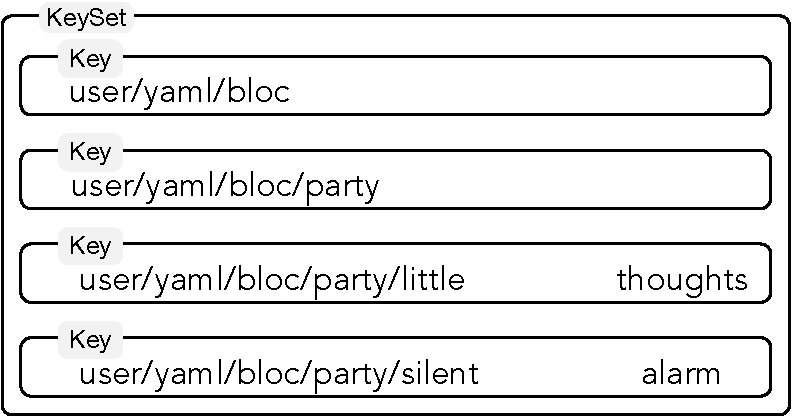
\includegraphics[width=.5\textwidth]{Keys}
  \caption{An exemplary \cc{KeySet}}
  \label{fig:keys}
\end{figure}

For example, the \cc{KeySet} shown in figure~\ref{fig:keys} would then map to the following \glstext{YAML} data, if we use \code{user/yaml} as mountpoint:

\begin{yamlcode}
  bloc:
  bloc/party:
  bloc/party/little: "thoughts"
  bloc/party/silent: "alarm"
\end{yamlcode}

. As we can see the resulting \glstext{YAML} file contains quite a lot of unnecessary redundant data.

In our second solution we take the hierarchical nature of the database into account and split on each part of a key. The result of this approach is the following \glstext{YAML} file:

\begin{yamlcode}
  bloc:
    party:
      little: "thoughts"
      silent: "alarm"
\end{yamlcode}

. The second solution removed unwanted redundancy and reflects the hierarchy much better. However, the approach also has an obvious downside: What happens if we want to store a value in \code{user/yaml/bloc} or \code{user/yaml/bloc/party}? To answer this question, let us look at a tree representing the \glstext{YAML} data from above.

\begin{figure}
  \centering
  \begin{subfigure}[t]{.4\textwidth}
    \centering
    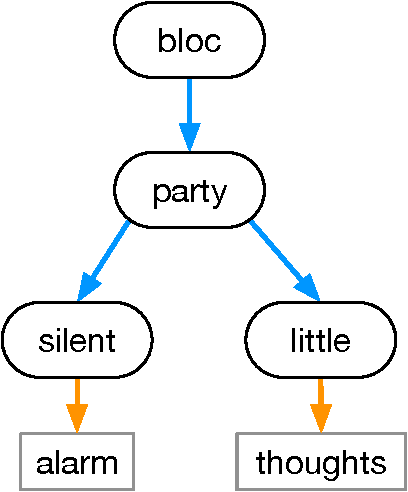
\includegraphics[height=4cm]{Tree}
    \caption{Initial representation}
    \label{fig:tree}
  \end{subfigure}
  \qquad
  \begin{subfigure}[t]{.4\textwidth}
    \centering
    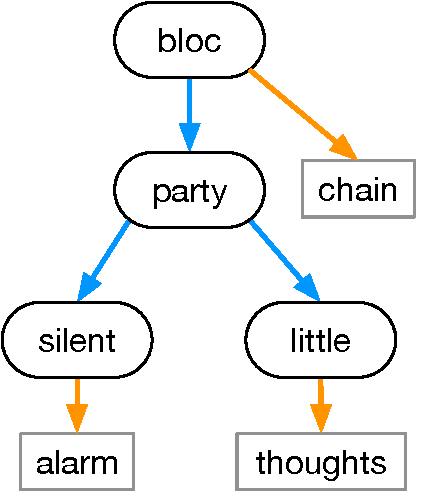
\includegraphics[height=4cm]{TreeExtended}
    \caption{We add an additional value}
    \label{fig:tree_extended}
  \end{subfigure}\\
  \begin{subfigure}[t]{.4\textwidth}
    \centering
    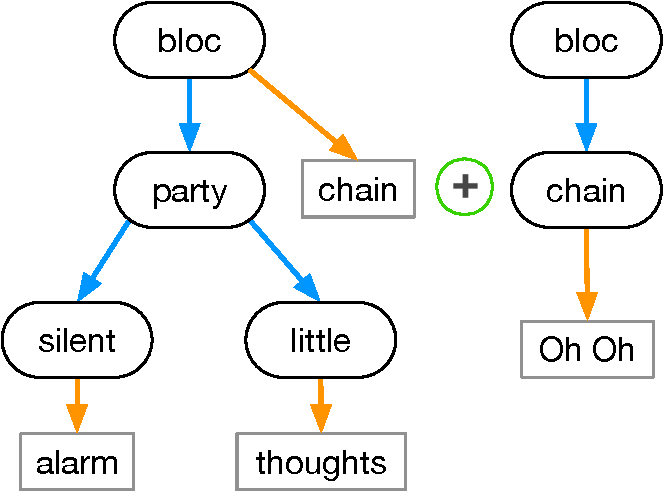
\includegraphics[height=4cm]{TreeExtended+}
    \caption{We add an additional \cc{Key} containing a value}
  \end{subfigure}
  \quad
  \begin{subfigure}[t]{.4\textwidth}
    \centering
    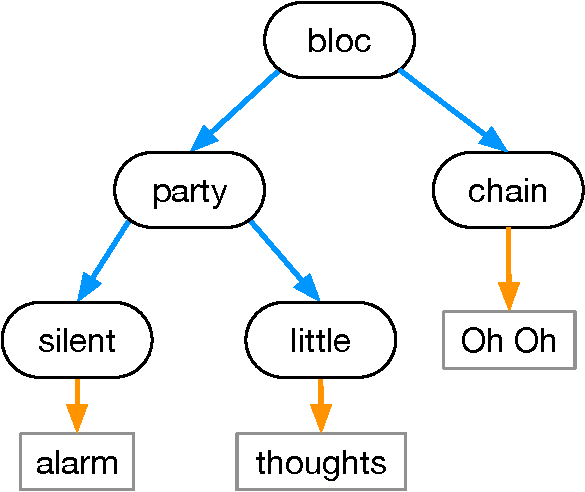
\includegraphics[height=4cm]{TreeExtended++}
    \caption{The new \cc{Key} overwrites the value of the node \code{block}}
    \label{fig:tree_extended++}
  \end{subfigure}
  \caption{The tree-like representation of \glstext{YAML} data shows the problem with adding non-leaf values}
\end{figure}

As we can see in Figure~\ref{fig:tree} the only nodes that store values are the leaves of the tree. Let us assume we also want to store the value \code{chain} in \code{user/yaml/bloc}. Figure~\ref{fig:tree_extended} shows the resulting tree. We could now save \code{chain} as a map key inside \code{bloc}:

\begin{yamlcode}
  bloc:
    chain:
    party:
      little: "thoughts"
      silent: "alarm"
\end{yamlcode}

. However using this approach we are unable to differentiate between the name and the value of a \cc{Key}. For example, if we add a new \cc{Key} with the name \code{user/yaml/bloc/chain} it would just overwrite the value of \code{user/yaml/bloc} (see Figure~\ref{fig:tree_extended++}).

Another option to fix our problem would be to use \glstext{YAML}’s list type, and to store the value of a \cc{Key} and the data below the \cc{Key} as first and second element of the list:

\begin{yamlcode}
  bloc:
    - chain                 # First element stores value
    - party:                # Second element stores data below
      -                     # `user/yaml/bloc/party` contains no value
      - little: "thoughts"
        silent: "alarm"
\end{yamlcode}

. However, this format is quite complicated. If we add support for Elektra’s array type – mapping arrays to \glstext{YAML} sequences – the situation is even worse.

To solve the problem we use another approach. We reserve the name \yaml{___dirdata} to save values in non-leaf nodes. The code below shows the mapping of our example data:

\begin{yamlcode}
  bloc:
    ___dirdata: "chain"
    party:
      little: "thoughts"
      silent: "alarm"
\end{yamlcode}

. Since we reserved the name \yaml{___dirdata} the value below this key will always be a leaf of the tree.

\subsection{Mapping Arrays}

Since Elektra’s array type and \glstext{YAML} sequences are similar, we want to map between these data types.

\begin{figure}
  \centering
    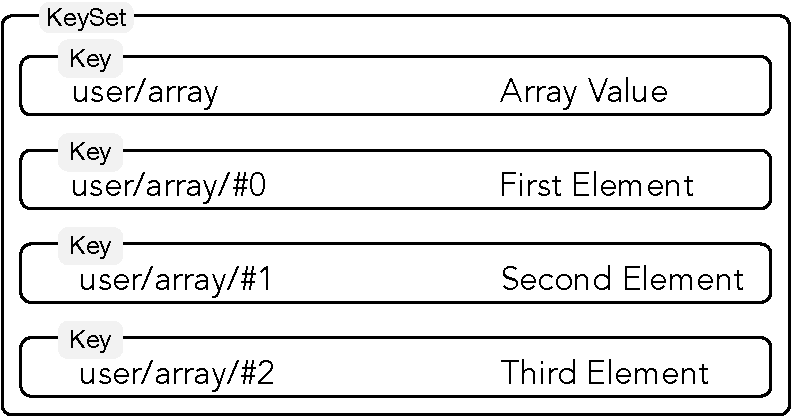
\includegraphics[width=.6\textwidth]{ArrayValue}
  \caption{The \cc{KeySet} above describes an array containing three elements}
  \label{fig:array_value}
\end{figure}

If we use this approach, then the \cc{KeySet} shown in Figure~\ref{fig:array_value} would result in the \glstext{YAML} data:

\begin{yamlcode}
  array:
    - "First Element"
    - "Second Element"
    - "Third Element"
\end{yamlcode}

. We are left with the problem, where to save the data of the \emph{parent} \cc{Key} of the array elements \code{user/array}. We can not use the same approach as before:

\begin{yamlcode}
  array:
    ___dirdata: "Array Value"
    - "First Element"
    - "Second Element"
    - "Third Element"
\end{yamlcode}

, since the result would be a \glstext{YAML} node that is neither sequence nor map. To fix this problem we decided to convert the \yaml{___dirdata} node to a sequence element:

\begin{yamlcode}
  array:
    - "___dirdata: Array Value"
    - "First Element"
    - "Second Element"
    - "Third Element"
\end{yamlcode}

. This approach produces valid \glstext{YAML} data and allows us to distinguish between array parents that store values and parents that do not, by checking the first array element for the value prefix \yaml{___dirdata:}.

\chapter{Implementation}

\section{Parsers}

\subsection{Recursive Descent Parser}

The first \href{https://github.com/ElektraInitiative/libelektra/commit/3d2d4644cb08e83f0b3305b8aeae546ada52dfe7}{version of the YAML plugin} developed in the course of this thesis used a handwritten recursive descent parser. As already described in “\nameref{sec:state_of_the_art}” this technique is quite popular, since there is a natural correspondence between code and grammar rules. Table~\ref{tab:recursive_descent_correspondence} shows the correspondence between \gls{ABNF} grammar rules and matching C like pseudo-code.

\begin{table}[H]
  \begin{center}
    \begin{tabular}{llp{0.48\textwidth}}
      \toprule
      Grammar & Example & Code\\
      \midrule

      Terminal
      &
      \texttt{{\color{color02} a}
              {\color{color03} \textbf{=}}
              {\color{color07} "a"}}
      &
        \begin{tabminted}[autogobble]{c}
          bool a() {
            bool match = getc(file) == 'a';
            if (!match) putc(file);
            return match;
          }
        \end{tabminted}
      \\

      Sequence
      &
      \texttt{{\color{color02} seq}
              {\color{color03} \textbf{=}}
              {\color{color02} rule1 rule2}}
      &
        \begin{tabminted}[autogobble]{c}
          bool seq() {
            return rule1() && rule2();
          }
        \end{tabminted}
      \\

      Alternative
      &
      \texttt{{\color{color02} seq}
              {\color{color03} \textbf{=}}
              {\color{color02} rule1}
              {\color{color03} /}
              {\color{color02} rule2}}
      &
        \begin{tabminted}[autogobble]{c}
          bool alt() {
            return rule1() || rule2();
          }
        \end{tabminted}
      \\

      \bottomrule
    \end{tabular}
  \end{center}
  \caption{Correspondence between grammar rules and code in a recursive descent parser}
  \label{tab:recursive_descent_correspondence}
\end{table}

\newpage
While Table~\ref{tab:recursive_descent_correspondence} suggest writing a recursive descent parser is trivial, there are many problems that the code above does not take into account:

\begin{description}
  \item [Recognizer Only:] The pseudo-code only implements a recognizer for the language. At the end of the parsing process we only know if the input is part of the language produced by the given grammar or not. Usually we want to \emph{build a data structure}, in our case a \cc{KeySet}, from the given input.

  \item [Error Handling:] The code does not contain any error handling. If a given input contains errors, then the creator or editor wants to know \emph{where these errors occurred}. Otherwise she or he has to check the whole input.

  \item [Left Recursion:] If we translate a left recursive rules such as \code{\color{color02} rule1 \color{color03} \textbf{=} \color{color02} rule1 \color{color03} / \color{color02} rule2} using the correspondences given in Table~\ref{tab:recursive_descent_correspondence}, then the resulting code would never terminate. This is the case, since \code{\color{color02} rule1} calls \code{{\color{color02} rule1}}, which then calls \code{\color{color02} rule1}, and so on an so forth (infinite recursion).
\end{description}

All of the problems above apply regardless of the programming language of the parsing code. Since we implemented the recursive descent parser in C, another issue is the error handling in C itself. The language does not provide a native exception handling mechanism. We therefore used the return value to also transfer the error information between functions. This approach is quite cumbersome, since it basically means that we have to check for an error after each function call.

We used C macros to minimize the code overhead and complexity caused by the error handling. Still, for a very small part of the YAML syntax described in the ABNF grammar of Figure~\ref{cod:abnf_recurive_descent} the parser contained about 374 lines of code (counted with \code{cloc} version 1.72). While smaller feature additions, such as going from support of one key-value pair to multiple key-value pairs \href{https://github.com/ElektraInitiative/libelektra/commit/17aa7a6ea5d9261287104213dcba67f4d0a0fcbc}{were quite straightforward} (\textcolor{Green}{14 additions}, \textcolor{Red}{1 deletion}), other modifications, such as supporting block styles would take considerable more effort.

Since the first steps with a hand-written recursive descent parser showed that this approach takes considerable effort we decided against extending the first prototype. Instead we chose to use an already existing hand-written YAML parser.

\begin{figure}[htbp]
  \centering
  \begin{code-boxed}
    {\small
{\color{color02} NEL} {\color{color03} \textbf{=}} {\color{color04} \%x85}{\color{color05} \\}{\color{color02} WSLF}
{\color{color03} \textbf{=}} {\color{color04} \textbf{WSP}} {\color{color03} \textbf{/}}
{\color{color04} \textbf{LF}}{\color{color05} \\\\}{\color{color06} ; Printable
characters from C0 set\\}{\color{color02} printable} {\color{color03} \textbf{=}}
{\color{color04} \textbf{HTAB}} {\color{color03} \textbf{/}} {\color{color04} \textbf{LF}}
{\color{color03} \textbf{/}} {\color{color04} \textbf{CR}}{\color{color05} \\}{\color{color06} ;
Printable ASCII\\}{\color{color02} printable} {\color{color03} \textbf{=/}} {\color{color04} \%x20}{\color{color03} \textbf{-}}{\color{color04} 7e}{\color{color05} \\}{\color{color06} ;
Next Line from C1 set\\}{\color{color02} printable} {\color{color03} \textbf{=/}}
{\color{color02} NEL}{\color{color05} \\}{\color{color06} ; Characters after C1
set -- Surrogate pairs\\}{\color{color02} printable} {\color{color03} \textbf{=/}}
{\color{color04} \%xa0}{\color{color03} \textbf{-}}{\color{color04} d7ff}{\color{color05} \\}{\color{color06} ;
Private use characters -- Replacement character\\}{\color{color02} printable}
{\color{color03} \textbf{=/}} {\color{color04} \%xe00}{\color{color03} \textbf{-}}{\color{color04} fffd}{\color{color05} \\}{\color{color06} ;
All Unicode Character Starting from the Supplementary Multilingual Plain\\}{\color{color02} printable}
{\color{color03} \textbf{=/}} {\color{color04} \%x10000}{\color{color03} \textbf{-}}{\color{color04} 10ffff}{\color{color05} \\\\}{\color{color02} pairs}
{\color{color03} \textbf{=}} {\color{color03} \textbf{*}}{\color{color02} WSLF}
{\color{color07} \texttt{"}\{\texttt{"}} {\color{color02} pair} {\color{color02} optionalAdditionalPairs}
{\color{color07} \texttt{"}\}\texttt{"}} {\color{color03} \textbf{*}}{\color{color02} WSLF}{\color{color05} \\}{\color{color02} optionalAdditionalPairs}
{\color{color03} \textbf{=}} {\color{color03} \textbf{*(}}{\color{color07} \texttt{"},\texttt{"}}
{\color{color02} pair}{\color{color03} \textbf{)}}{\color{color05} \\}{\color{color02} pair}
{\color{color03} \textbf{=}} {\color{color02} key} {\color{color07} \texttt{"}:\texttt{"}}
{\color{color02} value}{\color{color05} \\}{\color{color02} key} {\color{color03} \textbf{=}}
{\color{color02} doubleQuotedSpace}{\color{color05} \\}{\color{color02} value}
{\color{color03} \textbf{=}} {\color{color02} doubleQuotedSpace}{\color{color05} \\}{\color{color02} doubleQuotedSpace}
{\color{color03} \textbf{=}} {\color{color03} \textbf{*}}{\color{color02} WSLF}
{\color{color02} doubleQuoted} {\color{color03} \textbf{*}}{\color{color02} WSLF}{\color{color05} \\}{\color{color02} doubleQuoted}
{\color{color03} \textbf{=}} {\color{color04} \textbf{DQUOTE}} {\color{color02} content}
{\color{color04} \textbf{DQUOTE}}{\color{color05} \\}{\color{color02} content}
{\color{color03} \textbf{=}} {\color{color03} \textbf{*}}{\color{color02} printable}
}

  \end{code-boxed}
  \caption{ABNF grammar for a very small regular subset of YAML}
  \label{cod:abnf_recurive_descent}
\end{figure}

\chapter{Evaluation}
\label{sec:evaluation}

In the evaluation phase of the work we compare our parser plugins. For that purpose we first describe our comparison criteria in the first section of this chapter. After that we measure and analyze the plugins according to each criteria in the following sections. At the end we determine the plugins that best fit our criteria.

\section{Goals}

The goal of this evaluation is to find one or more parser plugin that
\begin{itemize}
  \item are fast,
  \item have low resource usage,
  \item use code that is
    \begin{itemize}
      \item both maintainable and
      \item easily extendible, and
    \end{itemize}
  \item has good error reporting capabilities.
\end{itemize}

To make sure that the plugins are reasonably fast we compare their execution time using runtime benchmarks and answer~\Cref{que:speed}.

  \speed*

For the resource usage we analyze the heap memory consumption. To make sure that the plugins are maintainable we analyze code sizes and take a look at the \glsdesc{CC}. We also examine the extensibility and composability of the plugins looking at code changes for specific bug fixes and feature additions. This step will help us to answer~\Cref{que:closeness}.

  \closeness*

To make sure the plugins produce good error messages we also compare these messages for specific input files in a detailed analysis.

\section{Performance Analysis}

In the following section we analyze the runtime time and memory usage of our plugins for certain input files. We first describe the overall methodical steps we took for both the runtime and memory benchmarks. Then we describe, measure and analyze both of these criteria in their own sections.

\subsection{Method}

To make all benchmarks reproducible we start by detailing the whole setup including used hardware, software, build configuration options and how we generated the input files.

\subsubsection{Hardware}

For all of the tests we used the hardware described in Table~\ref{table:benchmark_hardware}.

\begin{table}[H]
  \caption{Hardware Setup}
  \label{table:benchmark_hardware}
  \centering
  \begin{tabular}{ll}
\toprule
\multicolumn{2}{c}{MacBook Pro (Retina, 15-inch, Late 2013)}\\
\midrule
               CPU &            i7-4960HQ\\
                   &              2.6 GHz\\
                   &        6 MB L3 Cache\\
                   &      128 MB L4 Cache\\
               RAM &                16 GB\\
                   &        1600 MHz DDR3\\
                HD &    Apple SSD SM1024F\\
                   &                 1 TB\\
\bottomrule
  \end{tabular}
\end{table}

\subsubsection{Software}

Table~\ref{table:benchmark_software} shows the overall software setup for the benchmarks. We tested the performance both on macOS and Linux. For the Linux setup we used the Mac version of Docker. The basis of the runtime benchmark is \href{https://github.com/ElektraInitiative/libelektra/commit/54a4c0194946917b7d093e0777f465619b2f3d6f}{commit 54a4c019} of Elektra’s code base, while we measured the memory usage using \href{https://github.com/ElektraInitiative/libelektra/commit/ea418f177a5e2707f59f61b5e130a596abdd1c56}{commit ea418f17}. No code of any of the tested plugins changed \href{https://github.com/ElektraInitiative/libelektra/compare/54a4c0194946917b7d093e0777f465619b2f3d6f...ea418f177a5e2707f59f61b5e130a596abdd1c56}{between those two commits}.

\begin{table}[H]
    \newcommand{\YAEP}{{\href{https://github.com/vnmakarov/yaep/commit/550de4cc5600d5f6109c7ebcfbacec51bf80d8d3}{YAEP 550de4cc}}}
    \caption{Software Setup}
    \label{table:benchmark_software}
    \begin{subtable}[t]{.45\linewidth}
      \centering
        \caption{Mac Setup}
        \label{table:benchmark_mac}
        \begin{tabular}{ll}
\toprule
                OS &        macOS 10.14.5\\
                   &                     \\
\midrule
          Compiler &          Clang 8.0.0\\
        Generators &          ANTLR 4.7.2\\
                   &          Bison 3.4.1\\
         Libraries &       yaml-cpp 0.6.2\\
                   &                \YAEP\\
                   &          PEGTL 2.8.0\\
    Other Software &         CMake 3.14.4\\
                   &          Ninja 1.9.0\\
                   &      hyperfine 1.5.0\\
                   &            cloc 1.82\\
\bottomrule
        \end{tabular}
    \end{subtable}
    \begin{subtable}[t]{.45\linewidth}
      \centering
        \caption{Linux Setup}
        \label{table:benchmark_docker}
        \begin{tabular}{ll}
\toprule
            Docker &    18.09.2, build 6247962\\
        Base Image & Debian sid (sid-20190506)\\
\midrule
         Compilers &     Clang 6.0.1/GCC 8.3.0\\
        Generators &               ANTLR 4.7.2\\
                   &               Bison 3.3.2\\
         Libraries &            yaml-cpp 0.6.2\\
                   &                     \YAEP\\
                   &               PEGTL 2.7.1\\
    Other Software &              CMake 3.13.4\\
                   &               Ninja 1.8.2\\
                   &           hyperfine 1.5.0\\
\bottomrule
        \end{tabular}
    \end{subtable}
\end{table}

\subsubsection{Build Setup}

The following list shows the \href{https://cmake.org}{CMake} options that we used for all benchmarks:

\begin{itemize}
  \item \sh{-GNinja},
  \item \sh{-DPLUGINS=ALL},
  \item \sh{-DCMAKE_BUILD_TYPE=Release},
  \item \sh{-DENABLE_LOGGER=OFF}, and
  \item \sh{-DENABLE_DEBUG=OFF}.
\end{itemize}

\subsubsection{Input}

\newcommand{\URLKeyFramesJSON}{https://master.libelektra.org/src/plugins/yajl/yajl/keyframes_complex.json}

\newcommand{\FileKeyFrames}{{%
\codebox{%
\href{http://rawdata.libelektra.org/tree/master/YAML/Input/keyframes.yaml}%
{\textcolor{black}{\texttt{keyframes.yaml}}}}%
}}
\newcommand{\FileCombined}{{%
\codebox{%
\href{http://rawdata.libelektra.org/tree/master/YAML/Input/combined.yaml}%
{\textcolor{black}{\texttt{combined.yaml}}}}%
}}
\newcommand{\FileGenerated}{{%
\codebox{%
\href{http://rawdata.libelektra.org/tree/master/YAML/Input/generated.yaml}%
{\textcolor{black}{\texttt{generated.yaml}}}}%
}}
\newcommand{\FileGeneratedHundredThousand}{{%
\codebox{%
\href{http://rawdata.libelektra.org/tree/master/YAML/Input/generated_100000.yaml}%
{\textcolor{black}{\texttt{generated\_100000.yaml}}}}%
}}
\newcommand{\FileGenerateYAML}{{%
\codebox{%
\href{https://master.libelektra.org/scripts/generate-yaml}%
{\textcolor{black}{\texttt{generate-yaml}}}}%
}}
\newcommand{\FileCutInput}{{%
\codebox{%
\href{http://rawdata.libelektra.org/tree/master/YAML/Scripts/cut_input}%
{\textcolor{black}{\texttt{cut\_input}}}}%
}}

As first input for the benchmarks we used a \href{\URLKeyFramesJSON}{JSON configuration file} of the \href{https://www.libelektra.org/plugins/yajl}{YAJL plugin} that we converted to block syntax using the \LinkYAMLCPP{} plugin. We then modified the exported data by removing all \yaml{!<!elektra/meta>} tags, which are not supported by the other \glstext{YAML} plugins. We call the resulting file \FileKeyFrames{} in the remainder of the thesis. This file and all other data of the benchmark is available here:

\begin{leftbar}
  \url{http://rawdata.libelektra.org/tree/master/YAML}
\end{leftbar}

. For another input file called \FileCombined{} we copy and pasted parts of test data and various other \glstext{YAML} files in Elektra’s repository into a single file. While the file content is nonsensical, it should at least contains a mix of \glstext{YAML} data that covers most of the code paths of the \glstext{YAML} plugins.

Since both of these files are relatively small, \FileKeyFrames{} contains 218 lines, while \FileCombined{} contains 152 lines, we also generated data using a Python script that we called \FileGenerateYAML{}. This script generates \glstext{YAML} maps using \href{https://en.wikipedia.org/wiki/Universally_unique_identifier}{\glspl{UUID}} as scalar keys and values. For the \glstext{YAML} scalars the script randomly selects one of the three flow scalar styles:

\begin{itemize}
  \item single quoted scalar,
  \item double quoted scalar, or
  \item plain scalar
\end{itemize}

. This always works since \glspl{UUID} contain no character sequence that has special meaning according to the \glstext{YAML} specification. Using this method we generated two files:

\begin{itemize}
  \item \FileGenerated{} that contains 10 000 lines, and

  \item \FileGeneratedHundredThousand{} that contains 100 000 lines
\end{itemize}

. We also created another script called \FileCutInput{} to generate additional smaller input files that contain the first 50000, 10000, 5000, 1000, 500, 100, 50, 10, 5 and 1 lines of \FileGeneratedHundredThousand{}.

\subsection{Runtime Performance}
\label{sec:run_time_performance}

\subsubsection{Method}

\newcommand{\FilePluginGetSet}{{%
\codebox{%
\href{https://master.libelektra.org/benchmarks/plugingetset.c}%
{\textcolor{black}{\texttt{benchmark\_plugingetset}}}}%
}}
\newcommand{\FileBenchmarkYAML}{{%
\codebox{%
\href{https://master.libelektra.org/scripts/benchmark-yaml.in}%
{\textcolor{black}{\texttt{benchmark-yaml}}}}%
}}
\newcommand{\FileBenchmarkRuntime}{{%
\codebox{%
\href{http://rawdata.libelektra.org/tree/master/YAML/Scripts/benchmark-runtime}%
{\textcolor{black}{\texttt{benchmark-runtime}}}}%
}}
\newcommand{\ToolHyperfine}{{%
\codebox{%
\href{https://github.com/sharkdp/hyperfine}%
{\textcolor{black}{\texttt{hyperfine}}}}%
}}

To compare the runtime performance we used the C application \FilePluginGetSet{} that opens an Elektra plugin using a specific configuration file. For the whole benchmark process we created a Bash script, called \FileBenchmarkYAML{}, that uses the benchmarking tool \ToolHyperfine{} to call \FilePluginGetSet{} using different \glstext{YAML} plugins. Figure~\ref{fig:benchmark} shows a diagram of this setup.

\begin{figure}[H]
  \centering
    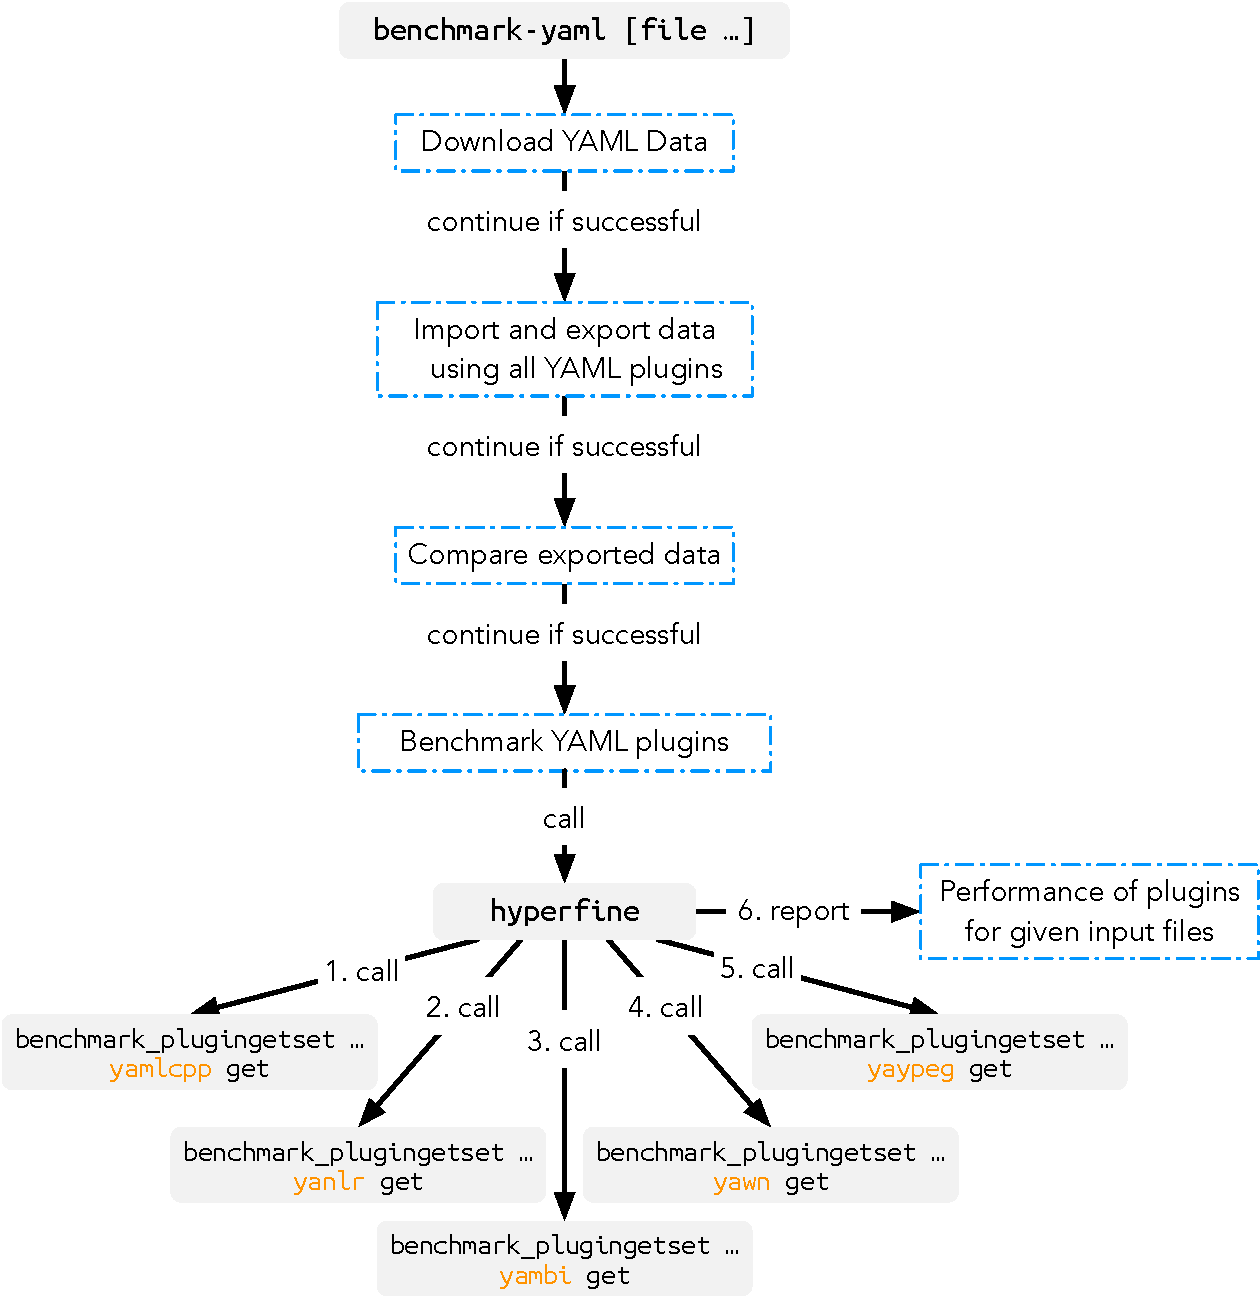
\includegraphics[width=0.9\textwidth]{Benchmark}
  \caption{The diagram above shows the basic sequence of steps to measure the runtime performance of the \glstext{YAML} plugins.}
  \label{fig:benchmark}
\end{figure}

For the measurement we use \ToolHyperfine{}, since this tool

\begin{enumerate}
  \item automatically determines how often it should call \FilePluginGetSet{} for meaningful measurement results,
  \item shows us when it is time to redo the benchmark, by informing us about statistical outliers, and
  \item prints important statistical data such as the mean runtime and the standard derivation.
\end{enumerate}

To make sure we repeat the benchmark every time \href{https://github.com/sharkdp/hyperfine}{\sh{hyperfine}} reports statistical outliers we created the Shell script \FileBenchmarkRuntime{}. This script calls \FileBenchmarkYAML{} for every input file and repeats a benchmark, until \href{https://github.com/sharkdp/hyperfine}{\sh{hyperfine}} does not report any warnings. The script \FileBenchmarkRuntime{} \emph{does} ignore warnings about runtimes under 5 milliseconds though, since \FilePluginGetSet{} might take less execution time for small \glstext{YAML} files.

\subsubsection{Results}

The graphs in this section show the results of the benchmark for different input files.

\begin{figure}[H]
  \begin{bchart}[max=30, width=0.8\textwidth, unit=ms]
    \bcbar[text=17.7 ± 0.7, value=macOS, color=orange]{17.7}
    \bcbar[text=25.5 ± 3.5, value=Linux/GCC, color=orange]{25.5}
    \bcbar[text=24.2 ± 2.9, value=Linux/Clang, color=orange]{24.2}

    \bcbar[text=15.8 ± 0.8, value=macOS, color=DarkYellow]{15.8}
    \bcbar[text=27.3 ± 2.3, value=Linux/GCC, color=DarkYellow]{27.3}
    \bcbar[text=25.8 ± 1.6, value=Linux/Clang, color=DarkYellow]{25.8}

    \bcbar[text=18.7 ± 1, value=macOS, color=Turquoise3]{18.7}
    \bcbar[text=20.1 ± 1.8, value=Linux/GCC, color=Turquoise3]{20.1}
    \bcbar[text=20.1 ± 1.6, value=Linux/Clang, color=Turquoise3]{20.1}

    \bcbar[text=13.8 ± 0.7, value=macOS, color=Aqua]{15.4}
    \bcbar[text=21.6 ± 1.8, value=Linux/GCC, color=Aqua]{21.6}
    \bcbar[text=19.8 ± 1.1, value=Linux/Clang, color=Aqua]{19.8}

    \bcbar[text=23.8 ± 1, value=macOS, color=DarkOrchid]{23.8}
    \bcbar[text=22.8 ± 2.2, value=Linux/GCC, color=DarkOrchid]{22.8}
    \bcbar[text=22.3 ± 2.1, value=Linux/Clang, color=DarkOrchid]{22.3}
  \end{bchart}
  \begin{center}
  \vspace{-0.5cm}
    \tikzcircle{orange} YAML CPP ~~
    \tikzcircle{DarkYellow} Yan LR ~~
    \tikzcircle{Turquoise3} YAMBi ~~
    \tikzcircle{Aqua} YAwn ~~
    \tikzcircle{DarkOrchid} YAy PEG
  \vspace{-0.5cm}
  \end{center}
  \caption{This bar chart shows the run time of the plugins for the input \FileKeyFrames{}.}
  \label{fig:benchmark_keyframes}
\end{figure}

\begin{figure}[H]
  \begin{bchart}[max=30, width=0.8\textwidth, unit=ms]
    \bcbar[text=12.3 ± 0.9, value=macOS, color=orange]{12.3}
    \bcbar[text=24.1 ± 2.7, value=Linux/GCC, color=orange]{24.1}
    \bcbar[text=22.2 ± 2.5, value=Linux/Clang, color=orange]{22.2}

    \bcbar[text=9.3 ± 0.5, value=macOS, color=DarkYellow]{9.3}
    \bcbar[text=24.6 ± 1.5, value=Linux/GCC, color=DarkYellow]{24.6}
    \bcbar[text=22.8 ± 1.5, value=Linux/Clang, color=DarkYellow]{22.8}

    \bcbar[text=11.9 ± 0.8, value=macOS, color=Turquoise3]{11.9}
    \bcbar[text=19.4 ± 1.4, value=Linux/GCC, color=Turquoise3]{19.4}
    \bcbar[text=18.9 ± 1.9, value=Linux/Clang, color=Turquoise3]{18.9}

    \bcbar[text=8.2 ± 0.6, value=macOS, color=Aqua]{8.2}
    \bcbar[text=20.2 ± 1.9, value=Linux/GCC, color=Aqua]{20.2}
    \bcbar[text=21.5 ± 4.2, value=Linux/Clang, color=Aqua]{21.5}

    \bcbar[text=14.3 ± 0.7, value=macOS, color=DarkOrchid]{14.3}
    \bcbar[text=20.3 ± 1.8, value=Linux/GCC, color=DarkOrchid]{20.3}
    \bcbar[text=19.7 ± 3.2, value=Linux/Clang, color=DarkOrchid]{19.7}
  \end{bchart}
  \begin{center}
  \vspace{-0.5cm}
    \tikzcircle{orange} YAML CPP ~~
    \tikzcircle{DarkYellow} Yan LR ~~
    \tikzcircle{Turquoise3} YAMBi ~~
    \tikzcircle{Aqua} YAwn ~~
    \tikzcircle{DarkOrchid} YAy PEG
  \vspace{-0.5cm}
  \end{center}
  \caption{This bar chart shows the run time of the plugins for the input \FileCombined{}.}
  \label{fig:benchmark_combined}
\end{figure}

\begin{figure}[H]
  \begin{bchart}[max=385, width=0.8\textwidth, unit=ms]
    \bcbar[text=239.5 ± 4.3, value=macOS, color=orange]{239.5}
    \bcbar[text=139.4 ± 2.8, value=Linux/GCC, color=orange]{139.4}
    \bcbar[text=137.3 ± 11.8, value=Linux/Clang, color=orange]{137.3}

    \bcbar[text=119.9 ± 1.1, value=macOS, color=DarkYellow]{119.9}
    \bcbar[text=123.7 ± 2.2, value=Linux/GCC, color=DarkYellow]{123.7}
    \bcbar[text=124.5 ± 5.2, value=Linux/Clang, color=DarkYellow]{124.5}

    \bcbar[text=174.8 ± 1.7, value=macOS, color=Turquoise3]{174.8}
    \bcbar[text=65 ± 2.4, value=Linux/GCC, color=Turquoise3]{65}
    \bcbar[text=64.8 ± 2.5, value=Linux/Clang, color=Turquoise3]{64.8}

    \bcbar[text=73.6 ± 1, value=macOS, color=Aqua]{73.6}
    \bcbar[text=77.3 ± 2.6, value=Linux/GCC, color=Aqua]{77.3}
    \bcbar[text=74.9 ± 3.1, value=Linux/Clang, color=Aqua]{74.9}

    \bcbar[text=363.2 ± 2, value=macOS, color=DarkOrchid]{363.2}
    \bcbar[text=156.8 ± 5.7, value=Linux/GCC, color=DarkOrchid]{156.8}
    \bcbar[text=161.1 ± 7.5, value=Linux/Clang, color=DarkOrchid]{161.1}
  \end{bchart}
  \begin{center}
  \vspace{-0.5cm}
    \tikzcircle{orange} YAML CPP ~~
    \tikzcircle{DarkYellow} Yan LR ~~
    \tikzcircle{Turquoise3} YAMBi ~~
    \tikzcircle{Aqua} YAwn ~~
    \tikzcircle{DarkOrchid} YAy PEG
  \vspace{-0.5cm}
  \end{center}
  \caption{This bar chart shows the run time of the plugins for the input \FileGenerated{}.}
  \label{fig:benchmark_generated}
\end{figure}

\begin{figure}[H]
  \centering
    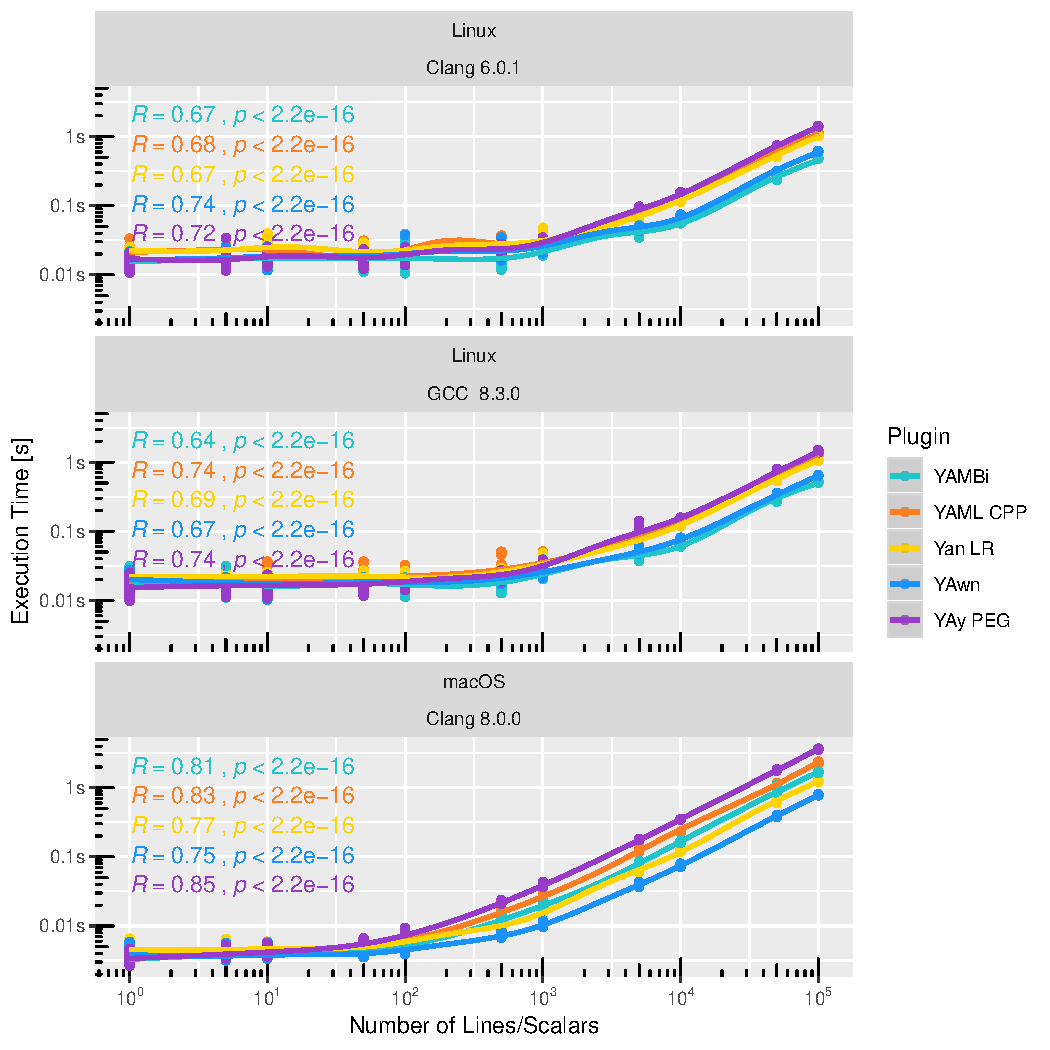
\includegraphics[width=\textwidth]{BenchmarkResultRuntime}
  \caption{The diagrams above show the runtime of the plugins for the input file \FileGeneratedHundredThousand{} and other files that contain only the first $n$ number of lines of this file.}
  \label{fig:benchmark_results_generated}
\end{figure}

\subsubsection{Analysis}

If we look at Figure~\ref{fig:benchmark_results_generated} we see that the runtime seems to grow linearly after a certain number of input lines. To verify this hypothesis we removed all samples with a line length smaller than 1000. Figure~\ref{fig:benchmark_results_generated_above_1000} shows the result.

\begin{figure}[H]
  \centering
    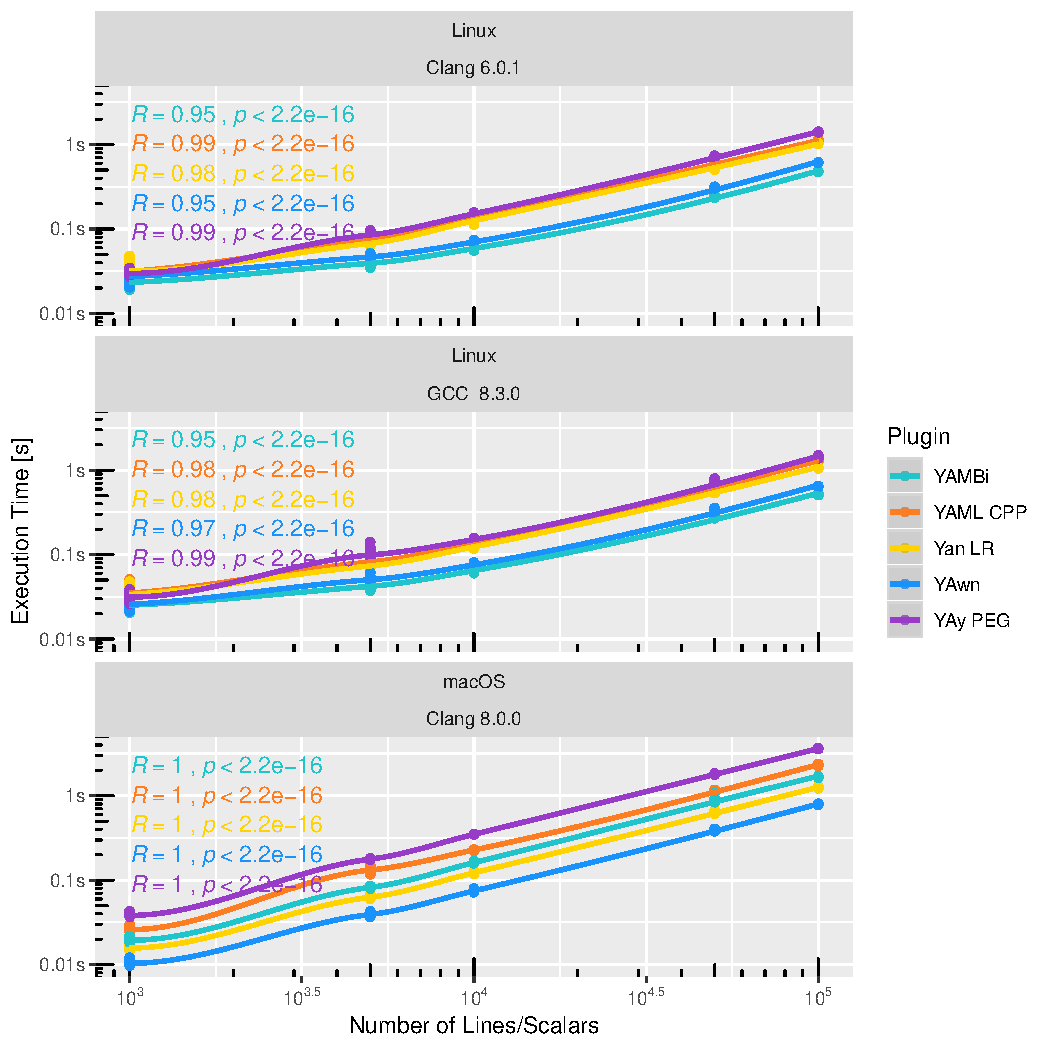
\includegraphics[width=\textwidth]{BenchmarkResultRuntimeAbove1000}
  \caption{The diagrams above shows that the runtime for the first lines of the file \FileGeneratedHundredThousand{} almost certainly grows linearly.}
  \label{fig:benchmark_results_generated_above_1000}
\end{figure}

From the correlation coefficients ($R$) of $0.95$ and higher we deduce that the runtime for all plugins almost certainly grows linearly. This means that the approximate runtime of the plugins should be the same. Now it is time to answer \Cref{que:speed}.

\speed*

The runtime of a non-backtracking recursive descent parser for an \glstext{LL}(1) grammar, as used by YAML CPP, should be $O(n)$. According to the literature the upper boundary for the runtime of

\begin{itemize}
  \item \gls{ALL(*)}, used by Yan LR, is $O(n⁴)$, but the algorithm often performs linearly~\cite[p. 1]{parr2014adaptive},
  \item LALR, used by YAMBi, is $O(n)$~\cite{baxter2017runtime},
  \item an Earley parser, used by YAwn, is $O(n²)$ for unambiguous grammars~\cite[p. 145]{hopcroft1969formal},
  \item a general PEG parsers, as used by YAy PEG, is exponential~\cite[p. 1]{moss2014derivatives} ($O(cⁿ)$) and for PEG parsers that use memoization is $O(n)$~\cite{ford2002packrat}
\end{itemize}

. We now compare the theoretic runtimes with the measured runtimes shown in Figure~\ref{fig:benchmark_results_generated_above_1000}. The text below lists some of our observations.

\begin{itemize}
  \item The deterministic (aka non-backtracking) parsers (YAML CPP, YAMBi) show the expected linear behavior.

  \item Yan LR also executes in linear time for the input. This is probably the result of the relatively simple grammar used by the parser. At least for all our input and test files we also checked that the grammar works with the simpler, but faster \gls{SLL(*)} strategy. This was indeed the case.

  \item YAwn also shows the linear behavior, even though \href{https://github.com/vnmakarov/yaep}{\gls{YAEP}} \href{https://github.com/vnmakarov/yaep/issues/24}{does not implement \citeauthor{leo1991general}’s optimization}~\cite{leo1991general} that makes sure that the algorithm runs in linear time for every \glstext{LR}(k) grammar.

  \item Even YAy PEG’s backtracking parser without memoization show linear behavior. As we already mentioned before in “\nameref{sec:state_of_the_art}” it is generally not clear, if memoization provides runtime improvements for a certain grammar. This seems also one of the reasons, why \gls{PEGTL} does not uses memoization, as can be seen in a quote of Colin Hirsch~\cite{hirsch2016memo}, one of the authors of \gls{PEGTL}, below.

  \begin{quote}
     …it would increase the complexity of the library beyond our design goals and only be useful in a very limited number of cases - in practice packrat parsers often perform worse than simple recursive descent parsers despite being in a better time complexity class.
  \end{quote}

\end{itemize}

Figure~\ref{fig:benchmark_generated} shows that the constant factor between the linear runtimes can be relatively high. For example on macOS, the fastest plugin YAwn is nearly five times faster than the slowest plugin YAy PEG for the file \FileGenerated{}:

\begin{equation}
  \frac{363.2\text{ms}}{73.6\text{ms}} ≅ 4.93
  \label{eq:benchmark_difference}
\end{equation}

. Other interesting observations concerning the runtime are listed below.

\begin{enumerate}
  \item The difference between the runtime of the fastest and slowest plugins for large files is nearly twice as large on macOS.

  \item The OS seems to play a much more important role, than the compiler for all of the used \glstext{YAML} libraries.

  \item While Yan LR and YAwn perform similarly on macOS and Linux, the difference between YAML CPP, YAMBi and YAy PEG on both operating systems can be quite significant.
\end{enumerate}

Since the runtime of the plugins is quite different on the two benchmarked operating systems we also determined mean of the mean values for the file \FileGenerated{}. We use a weight of

\begin{itemize}
  \item $0.5$ for the combination macOS/Clang,
  \item $0.25$ for the combination Linux/Clang, and
  \item $0.25$ for the combination Linux/GCC
\end{itemize}

and obtain the formula:

\begin{equation}
  \overline{t} = 0.5  · \overline{t}_{\text{macOS/Clang}} +
                 0.25 · \overline{t}_{\text{Linux/GCC}} +
                 0.25 · \overline{t}_{\text{Linux/Clang}}
  \label{eq:benchmark_generated_mean}
\end{equation}

. Figure \ref{fig:benchmark_generated_mean} shows a bar graph with the result of this calculation.

\begin{figure}[H]
  \begin{bchart}[max=300, width=0.8\textwidth, unit=ms]

    \bcbar[text=188.9, value=, color=orange]{188.9}

    \bcbar[text=122, value=, color=DarkYellow]{122}

    \bcbar[text=119.9, value=, color=Turquoise3]{119.9}

    \bcbar[text=74.9, value=, color=Aqua]{74.9}

    \bcbar[text=261, value=, color=DarkOrchid]{261}
  \end{bchart}
  \begin{center}
  \vspace{-0.5cm}
    \tikzcircle{orange} YAML CPP ~~
    \tikzcircle{DarkYellow} Yan LR ~~
    \tikzcircle{Turquoise3} YAMBi ~~
    \tikzcircle{Aqua} YAwn ~~
    \tikzcircle{DarkOrchid} YAy PEG
  \vspace{-0.5cm}
  \end{center}
  \caption{This bar chart shows the mean of the mean run times of the plugins according to Equation~\ref{eq:benchmark_generated_mean} for the input \FileGenerated{}.}
  \label{fig:benchmark_generated_mean}
\end{figure}

\subsubsection{Conclusion}

We determined with a high confidence that all of the \glstext{YAML} plugins show a linear runtime behavior (see Figure~\ref{fig:benchmark_results_generated_above_1000}), at least for the file \FileGeneratedHundredThousand{}. This puts all plugins, into the same computational complexity class. The constant difference between the runtime can still be relatively high though, as we can see in Equation~\ref{eq:benchmark_difference}.

The fastest plugin according to the mean of the mean runtimes (see Figure~\ref{fig:benchmark_generated_mean}) is YAwn, if we weigh the results of the two tested operating systems equally. This is interesting, since \citeauthor{earley1970efficient} himself mentions in his dissertation~\cite[p. 122]{earley1970efficient} that his parsing technique was too slow for practical use at the time, as you can see in the quote below.

\begin{quote}
  First we ask, what impact will our algorithm have on the parsing done in production compilers for existing programming languages? The answer is, practically none. Production compilers require guessing time proportional to n with a fairly low coefficient of n.
\end{quote}

Yan LR and YAMBi showed the second best runtimes, and were about $1.6$ times slower than YAwn. YAML CPP, which was, according to the results of Figure~\ref{fig:benchmark_generated_mean}, about $2.5$ times slower than Yawn takes the second to last place. Yay PEG was the slowest plugin on both tested operating systems, and is about $3.5$ times slower than the fastest plugin according to Figure~\ref{fig:benchmark_generated_mean}.

\subsection{Memory Usage}
\label{sec:memory_usage}

\subsubsection{Method}

\newcommand{\FileBenchmarkMemory}{{%
\href{http://rawdata.libelektra.org/tree/master/YAML/Scripts/benchmark-memory}%
{\sh{benchmark-memory}}%
}}

We measured the heap memory usage with the heap profiler \href{http://valgrind.org/docs/manual/ms-manual.html}{Massif}. Most of the other setup is similar to the one we used for the runtime benchmark, described in the section “\nameref{sec:run_time_performance}”. We still use the the C application \FilePluginGetSet{} to execute the plugins. The input files are also the same as before.

This time we do not need to determine the mean value of the results. Massif always produces the same output on the same hardware/software combination, since it runs the instrumented program \FilePluginGetSet{} on a “synthetic CPU”~\cite{valgrind2019core}.

To automate the process of measuring the memory usage for the different input files, we created a Shell script called \FileBenchmarkMemory{}. We only benchmarked the memory usage on Linux, since Massif did not support macOS 10.14 at the time we executed the benchmark script.

\subsubsection{Results}

The graphs in this section show the results of the memory benchmark for different input files.

\begin{figure}[H]
  \begin{bchart}[max=25, width=0.8\textwidth, unit=MB]
    \bcbar[text=17.5, value=Linux/GCC, color=orange]{17.5}
    \bcbar[text=18.3, value=Linux/Clang, color=orange]{18.3}

    \bcbar[text=23.8, value=Linux/GCC, color=DarkYellow]{23.8}
    \bcbar[text=23.8, value=Linux/Clang, color=DarkYellow]{23.8}

    \bcbar[text=10.4, value=Linux/GCC, color=Turquoise3]{10.4}
    \bcbar[text=10.1, value=Linux/Clang, color=Turquoise3]{10.1}

    \bcbar[text=9, value=Linux/GCC, color=Aqua]{9}
    \bcbar[text=8.8, value=Linux/Clang, color=Aqua]{8.8}

    \bcbar[text=22.8, value=Linux/GCC, color=DarkOrchid]{22.8}
    \bcbar[text=23.1, value=Linux/Clang, color=DarkOrchid]{23.1}
  \end{bchart}
  \begin{center}
  \vspace{-0.5cm}
    \tikzcircle{orange} YAML CPP ~~
    \tikzcircle{DarkYellow} Yan LR ~~
    \tikzcircle{Turquoise3} YAMBi ~~
    \tikzcircle{Aqua} YAwn ~~
    \tikzcircle{DarkOrchid} YAy PEG
  \vspace{-0.5cm}
  \end{center}
  \caption{This bar chart shows the peak heap memory usage of the plugins for the input \FileKeyFrames{}.}
  \label{fig:benchmark_memory_keyframes}
\end{figure}

\begin{figure}[H]
  \begin{bchart}[max=25, width=0.8\textwidth, unit=MB]
    \bcbar[text=12.6, value=Linux/GCC, color=orange]{12.6}
    \bcbar[text=12.9, value=Linux/Clang, color=orange]{12.9}

    \bcbar[text=17.5, value=Linux/GCC, color=DarkYellow]{17.5}
    \bcbar[text=17.4, value=Linux/Clang, color=DarkYellow]{17.4}

    \bcbar[text=7.7, value=Linux/GCC, color=Turquoise3]{7.7}
    \bcbar[text=7.6, value=Linux/Clang, color=Turquoise3]{7.6}

    \bcbar[text=7.9, value=Linux/GCC, color=Aqua]{7.9}
    \bcbar[text=7.8, value=Linux/Clang, color=Aqua]{7.8}

    \bcbar[text=14.8, value=Linux/GCC, color=DarkOrchid]{14.8}
    \bcbar[text=14.8, value=Linux/Clang, color=DarkOrchid]{14.8}
  \end{bchart}
  \begin{center}
  \vspace{-0.5cm}
    \tikzcircle{orange} YAML CPP ~~
    \tikzcircle{DarkYellow} Yan LR ~~
    \tikzcircle{Turquoise3} YAMBi ~~
    \tikzcircle{Aqua} YAwn ~~
    \tikzcircle{DarkOrchid} YAy PEG
  \vspace{-0.5cm}
  \end{center}
  \caption{This bar chart shows the peak heap memory usage of the plugins for the input \FileCombined{}.}
  \label{fig:benchmark_memory_combined}
\end{figure}

\begin{figure}[H]
  \begin{bchart}[max=700, width=0.8\textwidth, unit=MB]
    \bcbar[text=526.4, value=Linux/GCC, color=orange]{526.4}
    \bcbar[text=555, value=Linux/Clang, color=orange]{555}

    \bcbar[text=483.5, value=Linux/GCC, color=DarkYellow]{483.5}
    \bcbar[text=480.9, value=Linux/Clang, color=DarkYellow]{480.9}

    \bcbar[text=200.8, value=Linux/GCC, color=Turquoise3]{200.8}
    \bcbar[text=190.3, value=Linux/Clang, color=Turquoise3]{190.3}

    \bcbar[text=164.3, value=Linux/GCC, color=Aqua]{164.3}
    \bcbar[text=156.5, value=Linux/Clang, color=Aqua]{156.5}

    \bcbar[text=668.9, value=Linux/GCC, color=DarkOrchid]{668.9}
    \bcbar[text=684.2, value=Linux/Clang, color=DarkOrchid]{684.2}
  \end{bchart}
  \begin{center}
  \vspace{-0.5cm}
    \tikzcircle{orange} YAML CPP ~~
    \tikzcircle{DarkYellow} Yan LR ~~
    \tikzcircle{Turquoise3} YAMBi ~~
    \tikzcircle{Aqua} YAwn ~~
    \tikzcircle{DarkOrchid} YAy PEG
  \vspace{-0.5cm}
  \end{center}
  \caption{This bar chart shows the peak heap memory usage of the plugins for the input \FileGenerated{}.}
  \label{fig:benchmark_memory_generated}
\end{figure}

\begin{figure}[H]
  \centering
    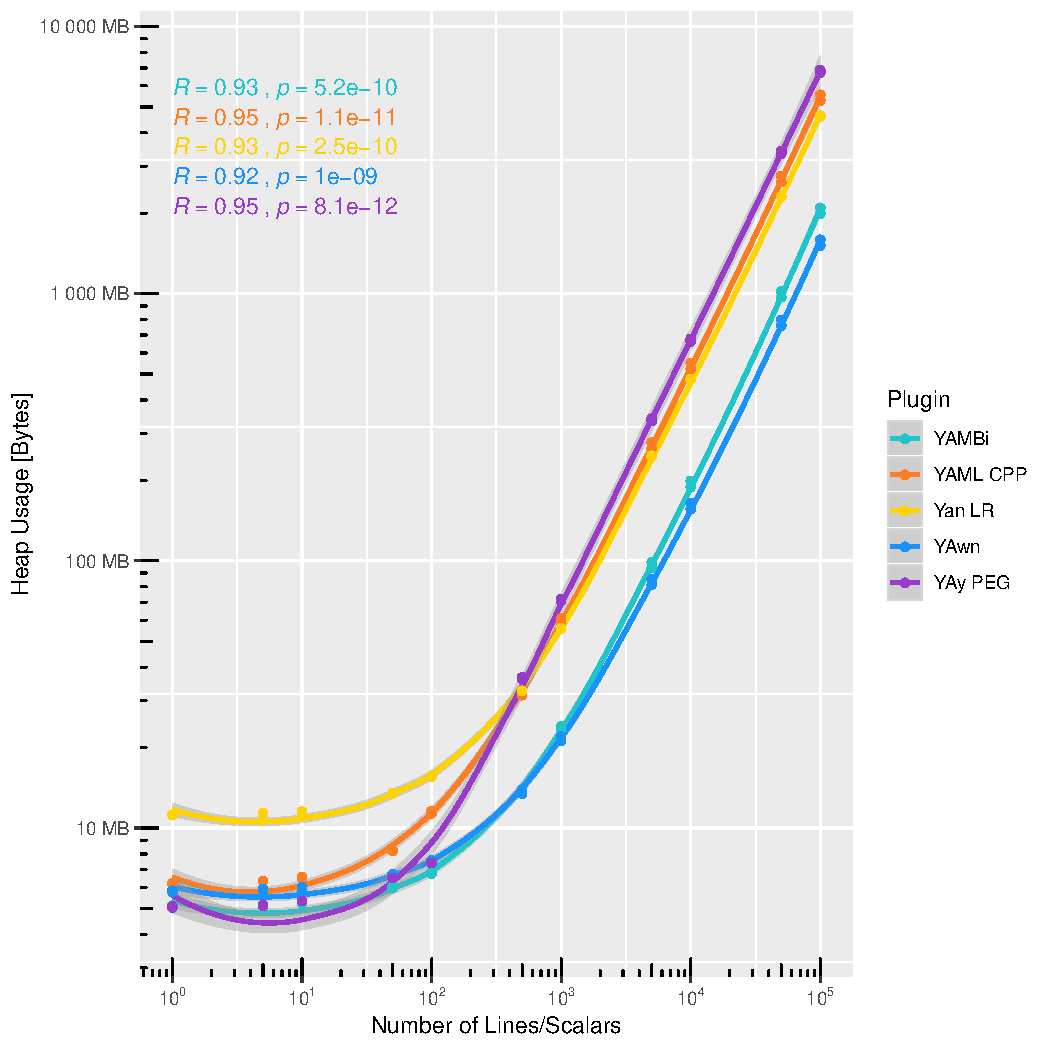
\includegraphics[width=\textwidth]{BenchmarkResultMemory}
  \caption{The diagrams above show the peak heap memory usage of the plugins for the input file \FileGeneratedHundredThousand{} and other files that contain only the first $n$ number of lines of this file.}
  \label{fig:benchmark_results_memory_lines}
\end{figure}

\subsubsection{Analysis}

Figure~\ref{fig:benchmark_results_memory_lines} shows that the memory usage seems to grow linearly for large line numbers. To analyze this behavior further, we limited the data for the graph to observation where the line number is 1000 or higher. Figure~\ref{fig:benchmark_results_memory_lines_above_thousand} shows the graph after this modification. From the correlation coefficients ($R$) of 1 and the low probabilities of the null hypothesis being wrong ($p$) we conclude that the memory consumption almost certainly grows linearly for all plugins.

\begin{figure}[H]
  \centering
    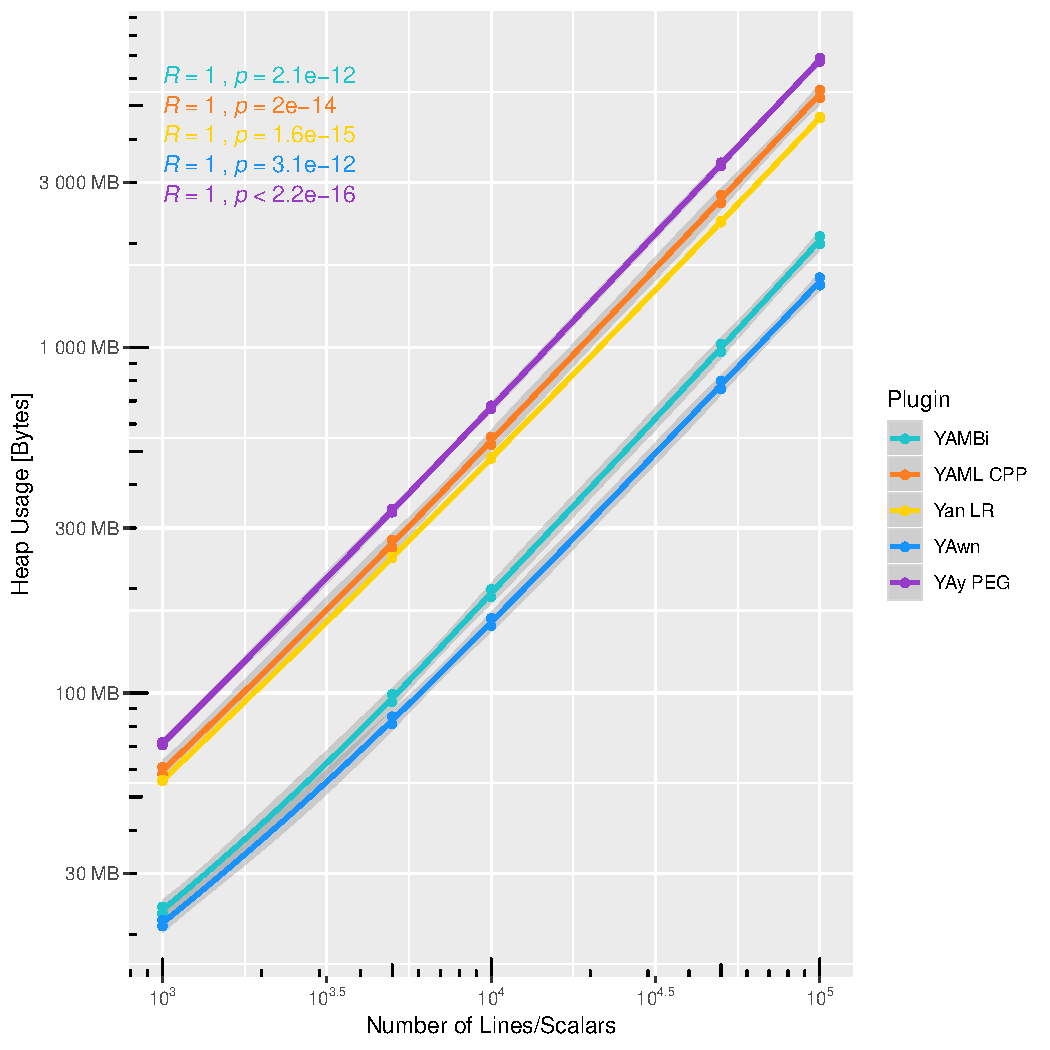
\includegraphics[width=\textwidth]{BenchmarkResultMemoryAbove1000}
  \caption{This diagram above shows that the memory usage of the \glstext{YAML} plugins almost certainly grows linearly for the first $n$ lines of the file \FileGeneratedHundredThousand{}}
  \label{fig:benchmark_results_memory_lines_above_thousand}
\end{figure}

\subsubsection{Conclusion}

While the asymptotic memory usage of all plugins grows linearly according to our measurements, the factor between the memory usage can be quite high. If we look at the data for the file \FileGenerated{} (see Figure~\ref{fig:benchmark_memory_generated}), then YAwn performs best, while YAMBi needs about $20\%$ more heap memory. The memory usage of the other plugins is much worse. Yan LR allocates about three times the heap memory of YAwn, YAML CPP takes about $3.4$ times the memory amount of YAwn, and YAy PEG needs even more than $4$ times the heap memory of YAwn.

\section{Code Size}
\label{sec:code_size}

\subsection{Method}

\newcommand{\FileCountLines}{{%
\codebox{%
\href{http://rawdata.libelektra.org/tree/master/YAML/Scripts/count-lines}%
{\textcolor{black}{\texttt{count-lines}}}}%
}}

We created a Shell script called \FileCountLines{} that counts the code lines of the \glstext{YAML} plugins using the tool \href{https://github.com/AlDanial/cloc}{cloc}. Since cloc \href{http://cloc.sourceforge.net/#Languages}{does not support Bison grammar files}, we wrote code that removes comments and empty lines from a Bison grammar, and afterwards counts the remaining lines using the Unix tool \sh{wc}.

\subsection{Results}

Figure~\ref{fig:line_count} shows the results reported by \FileCountLines{}. As you can see, we did not have to write a grammar for the library based YAML CPP plugin. For the other plugins, we either created a grammar (Yan LR, YAMBi, YAwn), or specified the grammar as handwritten code (Yay PEG). Only the \gls{ANTLR} (Yan LR) and Bison (YAMBi) based plugins use generated code. YAwn, which is based on \gls{YAEP}, uses the grammar directly.

\begin{figure}[H]
  \begin{bchart}[max=2100, width=0.75\textwidth, unit={~Lines of Code}]
    \bcbar[text=609, value=Handwritten, color=orange]{609}

    \bcbar[value=24 ~ Grammar, color=DarkYellow]{24}
    \bcbar[text=717, value=Handwritten, color=DarkYellow]{717}
    \bcbar[text=1108, value=Generated, color=DarkYellow]{1108}

    \bcbar[value=86 ~ Grammar, color=Turquoise3]{86}
    \bcbar[text=766, value=Handwritten, color=Turquoise3]{766}
    \bcbar[text=2046, value=Generated, color=Turquoise3]{2046}

    \bcbar[value=50 ~ Grammar, color=Aqua]{50}
    \bcbar[text=1096, value=Handwritten, color=Aqua]{1096}

    \bcbar[text=1187, value=Handwritten, color=DarkOrchid]{1187}
  \end{bchart}
  \begin{center}
  \vspace{-0.5cm}
    \tikzcircle{orange} YAML CPP ~~
    \tikzcircle{DarkYellow} Yan LR ~~
    \tikzcircle{Turquoise3} YAMBi ~~
    \tikzcircle{Aqua} YAwn ~~
    \tikzcircle{DarkOrchid} YAy PEG
  \vspace{-0.5cm}
  \end{center}
  \caption{This bar chart shows the line counts of of the \glstext{YAML} plugins.}
  \label{fig:line_count}
\end{figure}

\subsection{Analysis}

The line counts of Figure~\ref{fig:line_count} show that YAML CPP requires the least amount of code. That results is not that surprising, considering that the plugin uses yaml-cpp, a library that already represents the \glstext{YAML} file using high-level abstract data structures. We can convert these data structures into Elektra’s \cpp{KeySet} structure relatively easily, keeping the code size of the plugin small.

For a fair size comparison we also have to take the library code itself into consideration. We use the command

\begin{shellcode}
  cloc --include-lang='C++,C/C++ Header' src include
\end{shellcode}

to determine the code size of version 0.6.2 of the yaml-cpp library. The command reports $8413$ lines of code, showing us that parsing the full \glstext{YAML} standard requires a relatively large amount of code.

If we look at the other YAML plugins, we had to write the least code for Yan LR, followed by YAMBi, YAwn, and YAy PEG. The higher line counts of YAMBi and YAwn compared to Yan LR are not that surprising, considering that we implemented some functionality already provided by ANTLR, for those plugins ourselves.

For YAMBi we wrote two classes,

\begin{itemize}
  \item one that represents the input for the lexer ($63$ code lines), and
  \item another class that stores data about a lexer symbol ($53$ code lines)
\end{itemize}

. The sum of the lines of code ($63 + 53 = 116$) explains the difference between the amount of handwritten code between Yan LR and YAMBi ($717 - 609 = 108$) pretty well.

For YAwn we also added a symbol ($69$ code lines) and input class ($101$ code lines) as we did for YAMBi. Additionally we added

\begin{itemize}
  \item tree walking code ($124$ code lines),
  \item a listener ($126$ code lines),
  \item an error listener ($94$ code lines), and
  \item classes storing positional information ($38$ code lines)
\end{itemize}

. The $552$ code lines mentioned above are responsible for about half of the code of the whole plugin ($\frac{1096}{2} = 548$).

YAy PEG, with its scanner-less parsing engine based on C++ templates, uses the most handwritten code. Just like for YAwn we wrote

\begin{itemize}
  \item tree walking code ($128$ lines of code), and
  \item a listener ($122$ lines of code)
\end{itemize}

for the plugin. The other handwritten code take care of parsing ($822$ code lines) and the communication between the plugin and Elektra ($115$ code lines). The amount of parsing code of YAy PEG is quite large, compared to the grammar code of the other plugins. However, we have to consider

\begin{itemize}
  \item that YAy PEG’s parsing code supports a subset of \glstext{YAML} that is a little bit larger, than the one of the lexer based parsing plugins (Yan LR, YAMBi, YAwn), and
  \item that the parsing code also takes care of the work usually done by a lexer
\end{itemize}

. If we look at the lexer based plugins, they use between $352$ (YAMBi) and $416$ (Yan LR) code lines for the lexer.

Handwritten code requires manual work, and is therefore the most interesting criteria when we compare the code size of the plugins. However, the difference between the amount of generated code between the ANTLR based Yan LR plugin ($1108$ code lines), and the Bison based YAMBi plugin ($2046$ code lines) is also interesting. One reason for the big difference might be that ANTLR also requires a runtime library, while Bison generates all code needed for the parser. Both of these approaches have advantages and disadvantages. While Bisons’ approach means no additional dependencies, ANTLR’s runtime library provides space advantages. If multiple programs on the same machine use an ANTLR based parser, they can use the same compiled code, which only has to be stored in memory and on disk once.

\subsection{Conclusion}

If we take the amount of handwritten plugin code as main criteria for the code size comparison, then YAML CPP takes the lead, requiring the least amount of code. This is not surprising, considering that the parsing code of the plugin is part of the external yaml-cpp library, and not part of the plugin code itself.

The parser based plugin with the least amount of code is the ANTLR based Yan LR. The main reason for this is, that ANTLR already generates code for functionality that we had to create ourselves for the other plugins. While writing this support code is usually not that hard, it is certainly an advantage that ANTLR already provides support for common tasks, such as tree walking.

\section{Code Complexity}
\label{sec:code_complexity}

\subsection{Method}

\newcommand{\FileCheckComplexity}{{%
\codebox{%
\href{http://rawdata.libelektra.org/tree/master/YAML/Scripts/measure-complexity}%
{\textcolor{black}{\texttt{measure-complexity}}}}%
}}

For the code complexity analysis we measured the \glsdesc{CC} (\glstext{CC}) of

\begin{itemize}
  \item the parsing libraries and generators,
  \item the generated code (Yan LR, YAMBi), and the
  \item handwritten plugin code
\end{itemize}

with the analyzer \href{http://www.lizard.ws}{lizard}. Since we had to measure the complexity of many different code parts and we wanted to improve the reproducibility of the measurement we created a script for this task called \FileCheckComplexity{}.

\subsection{Results}

Table~\ref{table:cyclomatic_complexity} shows some of the values we measured via \FileCheckComplexity{}.

\begin{table}[H]
  \begin{adjustbox}{max width=\textwidth}
  \begin{threeparttable}
  \caption{The table below shows the measurement results of the script \FileCheckComplexity{}.}
  \label{table:cyclomatic_complexity}
  \centering
  \begin{tabular}{llrrrrrr}
\toprule
     Plugin &                    Part & \glstext{NLOC} & Average \glstext{CC} & Warnings & Function RT & \glstext{NLOC} RT\\
\midrule
   YAML CPP &                yaml-cpp &           7841 &                  2.5 &        7 &        0.01 &              0.09\\
            &                  Plugin &            556 &                  4.6 &        0 &           0 &                 0\\
\midrule
     Yan LR & \gls{ANTLR} C++ Runtime &          15760 &                  2.3 &       18 &        0.01 &              0.15\\
            &                  Plugin &            610 &                  2.1 &        0 &           0 &                 0\\
            &          Generated Code &           1105 &                  1.4 &        0 &           0 &                 0\\
\midrule
      YAMBi &                   Bison &          12677 &                  4.8 &       22 &        0.04 &              0.28\\
            &                  Plugin &            667 &                  2.3 &        0 &           0 &                 0\\
            &          Generated Code &           1526 &                  2.9 &        8 &        0.07 &              0.42\\
\midrule
       YAwn &                    YAEP &           5944 &                  3.9 &       10 &        0.04 &              0.28\\
            &                  Plugin &            990 &                  2.5 &        0 &           0 &                 0\\
\midrule
    YAy PEG &                   PEGTL &           8858 &                  1.6 &        4 &        0.01 &              0.05\\
            &                  Plugin &           1094 &                  2.9 &        0 &           0 &                 0\\
\bottomrule
  \end{tabular}

  \vspace{0.2cm}
  \begin{tablenotes}
    \item
        \hspace{1.65cm}
        \glstext{CC}…\glsdesc{CC}
        \hspace{1.7cm}
        \glstext{NLOC}…\glsdesc{NLOC}
    \item
      \[
       \text{Function RT} = \frac{\text{Warnings}}{\text{Number of Functions}}\quad
       \text{NLOC RT} = \frac{\text{NLOC with Warnings}}{\text{NLOC inside Functions}}
      \]
  \end{tablenotes}

  \end{threeparttable}
  \end{adjustbox}
\end{table}

\subsection{Analysis}

The most interesting parts of Table~\ref{table:cyclomatic_complexity} are the last two columns that show the relative amount of code that has a higher cyclomatic complexity than $15$. None of the handwritten plugin code contains any function with a \gls{CC} over this threshold. This is the result of using the static code analyzer \href{http://oclint.org}{OCLint} to check the code while we developed the plugins. Other than that, only the code generated by \gls{ANTLR} contains no code with a cyclomatic complexity over $15$. The cyclomatic complexity of the generated code by Bison is higher, which does not seem that surprising considering that \glstext{LR} parsers, contrary to \glstext{LL} parser, are almost never written by hand, because of their inherent complexity. If we look at the parser libraries and parser generators themselves, \gls{PEGTL} is the library containing the least amount of code over the complexity threshold, followed by yaml-cpp, and ANTLR’s C++ runtime. Bison and \gls{YAEP} are the generator and library that contain the most code with a high cyclomatic complexity.

\subsection{Conclusion}

While cyclomatic complexity has “never been unambiguously correlated with defective or unmaintainable code”~\cite{martin2017c++}, the measurements in this section provide at least some indication about code that might be problematic due to a high code complexity.

\section{Ease of Extensibility and Composability}
\label{sec:extensibility}

One advantage of parsing libraries and parser generators over handwritten parsers is that we can update the language grammar without having to rewrite parsing code. This way we can extend the parsed \glstext{YAML} subset easily without many manual code changes. In the first part of the next section we analyze how many code line changes it took to, fix bugs in, and add minor features to, the \glstext{YAML} plugins. The amount of code changes provides a good metric on how much effort it takes to extend the parser plugins.

In the second part of this section we will take a look at how the composability of our parsing code influences the extensibility. One option to create an extensible system is to base it on components. We can reuse these components to keep the amount of code for a new feature or bug fix low. We can imagine that the rules of a grammar represent components in our parsing systems. Parsing systems without a separate lexing phase such as PEGTL take the composability idea one step further. In PEGTL we can compose the parser for the whole grammar out of smaller parser that build on each other. We will analyze, if the component based parser of YAy PEG provides extensibility advantages over the other parsers. We will also answer~\Cref{que:closeness} in this part of the thesis.

\closeness*

\subsection{Plugin Updates}

In the next subsections we look at the effort it took to, add certain features to, and fix certain bugs in, the \glstext{YAML} plugins.

\subsubsection{Method}

As measurement for the extendibility effort we use the amount of changed code lines. Since we want to keep the comparison fair, we only look at the code changes needed for a certain feature or bug fix, excluding additional test code and documentation updates.

\subsubsection{Support for Elektra’s Boolean Data Type}

Elektra’s \cc{Key} data structure usually saves data as untyped character string. We can add type information for a certain key by adding a \code{type} meta key (see also Section “\nameref{sec:keyset}”). If we do that Elektra ensures that applications store and retrieve the right kind of data for that specific key. Elektra’s C++ \gls{API} offers a direct way to store and retrieve a typed value via templated functions. We used these functions to improve the support for boolean data types in the \glstext{YAML} plugins.

\glstext{YAML}’s JSON schema represents boolean data as scalar with the canonical value \yaml{false} or \yaml{true}~\cite{ben2009yaml}. More advanced schemas, such as the core schema offer additional aliases for true and false values. For the \glstext{YAML} plugins in this thesis we only added support for the JSON schema though. For this to work we had to translate the \glstext{YAML} values \yaml{false} and \yaml{true} to \href{https://master.libelektra.org/doc/decisions/bool.md}{Elektra’s boolean values} \code{0} and \code{1}.

Just like Elektra’s C++ \gls{API}, yaml-cpp, the library used by the YAML CPP plugin, also offers templated functions to retrieve and set boolean values. One problem of yaml-cpp’s \gls{API} is that there seems to be no way to check for the type of a \glstext{YAML} node, without the possibility of throwing an exception~\cite{beder2013type}. This can be problematic for the runtime efficiency, since YAML CPP might trigger multiple exceptions before it converts a \glstext{YAML} node to a correctly typed Elektra key. To improve the runtime performance of YAML CPP we checked the textual value of a \glstext{YAML} node before we converted it. The implementation of this more \href{https://github.com/ElektraInitiative/libelektra/commit/d4e62eebd006ea4b066c75e6e885ee5a4b6e26cf#diff-4bdb640234f370e3a9db751e1f7d769b}{complicated approach} modified $16$ code lines (\textcolor{Green}{$15$ additions}, \textcolor{Red}{$1$ deletion}), while the implementation of the \href{https://github.com/ElektraInitiative/libelektra/commit/1e9a07baad8a140c6eda654053db450c0901f5d0#diff-4bdb640234f370e3a9db751e1f7d769b}{direct approach} – that might cause more exceptions for data without many boolean values – modified only $9$ additional code lines (\textcolor{Green}{$8$ additions}, \textcolor{Red}{$1$ deletion}).

Adding support for boolean values modified $10$ lines in \href{https://issues.libelektra.org/2653}{Yan LR’s} code base (\textcolor{Green}{$9$ additions}, \textcolor{Red}{$1$ deletion}), and $9$ lines (\textcolor{Green}{$8$ additions}, \textcolor{Red}{$1$ deletion}) in each of the other plugins (\href{https://issues.libelektra.org/2652}{YAMBI}, \href{https://issues.libelektra.org/2651}{YAwn}, \href{https://issues.libelektra.org/2654}{YAy PEG}). The similar line counts are a direct result of all of the plugins using a listener interface to convert parsed \glstext{YAML} data. To add boolean support we only had to change code in one of the functions of the listeners.

\begin{figure}[H]
  \begin{bchart}[max=20, width=0.8\textwidth, unit={~Lines of Code}]
    \bcbar[text=9, value=Direct Approach, color=orange]{9}
    \bcbar[text=16, value=Complex Approach, color=orange]{16}
    \bcbar[text=10, value=, color=DarkYellow]{10}
    \bcbar[text=9, value=, color=Turquoise3]{9}
    \bcbar[text=9, value=, color=Aqua]{9}
    \bcbar[text=9, value=, color=DarkOrchid]{9}
  \end{bchart}
  \begin{center}
  \vspace{-0.5cm}
    \tikzcircle{orange} YAML CPP ~~
    \tikzcircle{DarkYellow} Yan LR ~~
    \tikzcircle{Turquoise3} YAMBi ~~
    \tikzcircle{Aqua} YAwn ~~
    \tikzcircle{DarkOrchid} YAy PEG
  \vspace{-0.5cm}
  \end{center}
  \caption{This bar chart shows the number of modified lines needed for adding better boolean support to the \glstext{YAML} plugins.}
  \label{fig:boolean_line_count}
\end{figure}

\subsubsection{Conversion of Empty Values}

Depending on the context, empty content (empty nodes) in a \glstext{YAML} stream might represent null values. Elektra should store these null values in a key with a zero length binary value. This was not the case in the first version of the parser based \glstext{YAML} plugins (Yan LR, YAMBi, YAwn, YAy PEG). Instead the plugins would incorrectly convert these null values into empty strings.

Another similar problem was that the lexer based plugins would not convert empty content null values right before the end of a file (\code{EOF}\glsadd{EOF}). The result of this bug was that the lexer would not terminate for a stream such as the one shown in Figure~\ref{fig:Figures_StreamNullEOF}.

\begin{figure}[H]
  \centering
    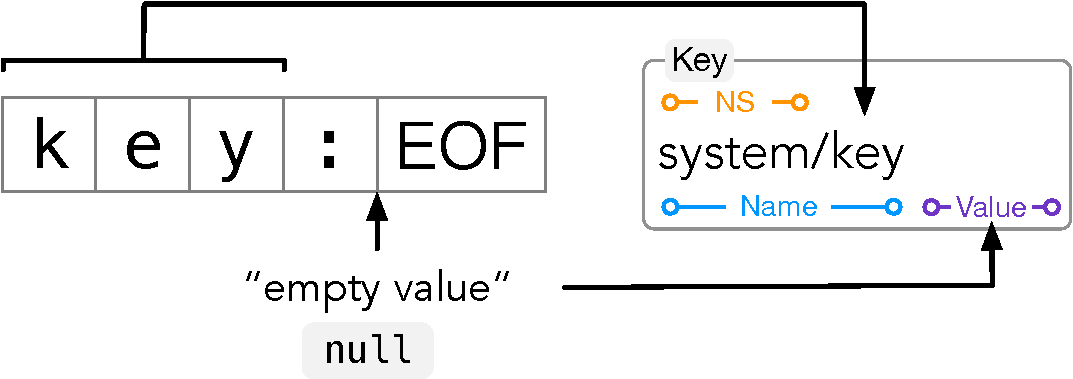
\includegraphics[width=0.75\textwidth]{StreamNullEOF}
  \caption{The \glstext{YAML} data on the left represents a map that contains one key-value pair with the name \code{key} that stores a null value. The \cc{Key} structure on the right shows the converted \glstext{YAML} data, if we store it directly below the \gls{NS} \code{system}.}
  \label{fig:Figures_StreamNullEOF}
\end{figure}

Figure~\ref{fig:null_line_count} shows the amount of changed lines for the \href{https://issues.libelektra.org/2662}{Yan LR}, \href{https://issues.libelektra.org/2663}{YAMBi}, \href{https://issues.libelektra.org/2664}{YAwn}, and \href{https://issues.libelektra.org/2665}{YAy PEG} plugin. The code changes for all the lexer based plugins (Yan LR, YAMBi, YAwn) are almost identical, since we had to fix the problems in the lexer and listener code, which is quite similar for all of those plugins.

For YAy PEG we only had to fix the support for empty nodes in the middle of a \glstext{YAML} stream, since YAy PEG’s parsing code already handled empty nodes at the end of a file correctly. This is probably a direct result of using grammar code that is quite similar to the one from the \href{http://yaml.org/spec/1.2/spec}{YAML specification}. The notable difference between the amount of code we added for the empty node fix (\textcolor{Green}{$5$ additions}, \textcolor{Red}{$1$ deletion}) compared to the one of the lexer based plugins (\textcolor{Green}{$1$ addition}) is also a result of YAy PEG’s grammar. YAy PEG uses the same code path to add empty and non-empty mapping values. The lexer based plugins on the other hand check for an empty value inside the listener code for a key-value pair. We could also use this approach in the YAy PEG plugin, but that would possibly require substantial code changes to the tree walking code.

\begin{figure}[H]
  \begin{bchart}[max=10, width=0.8\textwidth, unit={~Lines of Code}]
    \bcbar[text=1, value=Empty Node, color=DarkYellow]{1}
    \bcbar[text=5, value=Empty Node Before EOF, color=DarkYellow]{5}
    \bcbar[text=1, value=Empty Node, color=Turquoise3]{1}
    \bcbar[text=4, value=Empty Node Before EOF, color=Turquoise3]{4}
    \bcbar[text=1, value=Empty Node, color=Aqua]{1}
    \bcbar[text=4, value=Empty Node Before EOF, color=Aqua]{4}
    \bcbar[text=6, value=Empty Node, color=DarkOrchid]{6}
  \end{bchart}
  \begin{center}
  \vspace{-0.5cm}
    \tikzcircle{orange} YAML CPP ~~
    \tikzcircle{DarkYellow} Yan LR ~~
    \tikzcircle{Turquoise3} YAMBi ~~
    \tikzcircle{Aqua} YAwn ~~
    \tikzcircle{DarkOrchid} YAy PEG
  \vspace{-0.5cm}
  \end{center}
  \caption{This bar chart shows the additional lines needed for fixing the null value support of the \glstext{YAML} plugins.}
  \label{fig:null_line_count}
\end{figure}

\subsubsection{Conversion of Empty Documents}

According to the \glstext{YAML} specification an empty file corresponds to a null value. We did not consider this in the initial versions of the \glstext{YAML} plugins, which meant the empty documents shown in Figure~\ref{fig:null_yaml} were translated incorrectly. Figure~\ref{fig:empty_document_count} shows the amount of code lines we modified to fix this problem for the \href{https://issues.libelektra.org/2711}{Yan LR}, \href{https://issues.libelektra.org/2712}{YAMBi}, \href{https://issues.libelektra.org/2713}{YAwn} and \href{https://issues.libelektra.org/2714}{YAy PEG} plugin.

\begin{figure}[H]
  \centering
  \begin{minipage}[c]{0.48\textwidth}
    \begin{code-boxed}
      \vspace{10pt}
    \end{code-boxed}
  \end{minipage}
  \begin{minipage}[t]{0.02\textwidth}~\end{minipage}
  \begin{minipage}[c]{0.48\textwidth}
    \begin{yamlcode}
      # Empty document
    \end{yamlcode}
  \end{minipage}
  \caption{The examples above show two options on how to store “nothing” (\code{null}) using \glstext{YAML}.}
  \label{fig:null_yaml}
\end{figure}

\begin{figure}[H]
  \begin{bchart}[max=20, width=0.8\textwidth, unit={~Lines of Code}]
    \bcbar[text=10, value=, color=DarkYellow]{10}
    \bcbar[text=17, value=, color=Turquoise3]{17}
    \bcbar[text=15, value=, color=Aqua]{15}
    \bcbar[text=10, value=, color=DarkOrchid]{10}
  \end{bchart}
  \begin{center}
  \vspace{-0.5cm}
    \tikzcircle{orange} YAML CPP ~~
    \tikzcircle{DarkYellow} Yan LR ~~
    \tikzcircle{Turquoise3} YAMBi ~~
    \tikzcircle{Aqua} YAwn ~~
    \tikzcircle{DarkOrchid} YAy PEG
  \vspace{-0.5cm}
  \end{center}
  \caption{This bar chart shows the amount of code lines we modified to fix the conversion of empty documents.}
  \label{fig:empty_document_count}
\end{figure}

\begin{sloppypar}
When we implemented the fixes for the empty document conversion we noticed that we added nearly identical code to the listener (Yan LR, YAwn, YAy PEG) respectively driver (YAMBi) of the plugins. These modifications took \textcolor{Green}{$6$ additions} for Yan LR and \textcolor{Green}{$5$ additions} for the other plugins. We should mention here that we could also have avoided two additional lines for the Yan LR plugin, which consisted of an \cpp{using} statement and the inclusion of an optional header file.
\end{sloppypar}

The other code line differences were a result of grammar updates to

\begin{itemize}
  \item Yan LR (\textcolor{Green}{$3$ additions}, \textcolor{Red}{$1$ deletion}),
  \item YAMBi (\textcolor{Green}{$7$ additions}, \textcolor{Red}{$5$ deletion}), and
  \item YAwn (\textcolor{Green}{$5$ additions}, \textcolor{Red}{$1$ deletion})
\end{itemize}

and updates to tree walking code of:

\begin{itemize}
  \item YAwn (\textcolor{Green}{$4$ additions}), and
  \item YAy PEG (\textcolor{Green}{$5$ additions})
\end{itemize}

. The relatively high number of changes to the grammar of YAMBi is deceiving, since we also moved a 4 line grammar block (\textcolor{Green}{$4$ additions}, \textcolor{Red}{$4$ deletion}) in the bug fix update for the plugin. Figure~\ref{fig:empty_document_minimum_count} takes this code block movement and the optional line changes for Yan LR into account to give a better overview of the code changes we needed to implement the bug fix.

\begin{figure}[H]
  \begin{bchart}[max=20, width=0.8\textwidth, unit={~Lines of Code}]
    \bcbar[text=8, value=, color=DarkYellow]{8}
    \bcbar[text=9, value=, color=Turquoise3]{9}
    \bcbar[text=15, value=, color=Aqua]{15}
    \bcbar[text=10, value=, color=DarkOrchid]{10}
  \end{bchart}
  \begin{center}
  \vspace{-0.5cm}
    \tikzcircle{orange} YAML CPP ~~
    \tikzcircle{DarkYellow} Yan LR ~~
    \tikzcircle{Turquoise3} YAMBi ~~
    \tikzcircle{Aqua} YAwn ~~
    \tikzcircle{DarkOrchid} YAy PEG
  \vspace{-0.5cm}
  \end{center}
  \caption{This bar chart shows the “minimal” code line modifications we needed to fix the conversion of empty documents.}
  \label{fig:empty_document_minimum_count}
\end{figure}

\subsection{Component Based Grammars and Extensibility}

The \href{http://yaml.org/spec/1.2/spec}{YAML specification} includes a detailed grammar description of the language in a parameterized \gls{BNF} like syntax. The grammar rules of the specification are very reminiscent of parser combinator functions~\cite{hutton1992higher, hutton1996monadic}. This is not that surprising considering that \href{https://hackage.haskell.org/package/YamlReference}{YAML’s reference parser} is also based on parser combinators. A large part of the reference parser actually uses slightly modified versions of all of the rules of the \glstext{YAML} spec. Since “the order of alternatives in the grammar is significant”~\cite{ben2009yaml} (ordered choice) and some of the parsing rules also uses positive and negative lookahead we can also categorize \glstext{YAML}’s reference grammar as an extended version of a \gls{PEG}.

In the section “\nameref{sec:peg_parser}” we already mentioned that the grammar description of the YAy PEG plugin resembles the \glstext{YAML} specification grammar quite closely. It is time to analyze, if this close resemblance provides advantages over the other \glstext{YAML} plugins, which use a description that is quite different to the one of the \glstext{YAML} specification.

Table~\ref{table:extensibility} lists some of the advantages and disadvantages we found while we implemented and extended the \glstext{YAML} plugins.

\begin{table}[H]
  \caption{The table below lists some advantage and disadvantages of PEG based (YAy PEG) and lexer based (Yan LR, YAMBi, YAwn) plugins regarding extensibility.}
  \label{table:extensibility}
  \centering
  \begin{tabular}{ll}
\toprule
                           \tikzcircle{DarkOrchid} YAy PEG & \tikzcircle{DarkYellow} \tikzcircle{Turquoise3} \tikzcircle{Aqua} Lexer Based Plugins\\
\midrule
\textcolor{Green}{+} Grammar Extension via “Copy \& Paste” &                                 \textcolor{Green}{+}                   Simple Grammar\\
                    \textcolor{Red}{–} Complicated Grammar &                                                 \textcolor{Red}{–} Handwritten Lexer\\
                              \textcolor{Red}{–} Debugging &                                                                                      \\
\bottomrule
  \end{tabular}
\end{table}

Using the PEG library certainly offers advantages considering the extensibility of the grammar, since we can more or less copy the grammar rules from the specification or reference parser and modify them slightly for \gls{PEGTL}. Fortunately the reference parser already contains a relatively large test suite, which means the chance of errors in the reference grammar is quite low. This is helpful, since the specification grammar consists of 211 rules, which can be quite complicated. This is also one of the disadvantages of using \gls{PEGTL}, since the grammar of YAy PEG is more complicated than the one of the lexer based plugins. The complexity is a result of using a single pass to parse \glstext{YAML} data instead of using a separate lexer and parser phase. The single parsing phase also makes debugging harder since we can not debug the lexer and parsing code separately.

Keeping the information above in mind we can now answer \Cref{que:closeness}.

  \closeness*

The parser of YAy PEG certainly stays closest to the grammar definition of the \glstext{YAML} specification. This closeness is helpful, if we look at the extension of the grammar. However, since YAy PEG’s grammar code also handles low level details of the parsing process we have to consider these details later in the parsing process, which reduces the extensibility of the parsing support code compared to the one of the lexer based plugins.

\subsection{Conclusion}

The examples at the start of this section show that the extensibility of the different \glstext{YAML} plugins depend on the specific bug we want to fix or the feature we like to add. Sometimes the code changes can be quite similar, at least for all the lexer based plugins (Yan LR, YAMBi, YAwn). Other times we need to change code in nearly all parts of a plugin. In these cases plugins that use generators and libraries that provide more built-in code support are easier to extend. If we take the built-in support code into account, then the order of ease of extensibility for the lexer based plugins is roughly Yan LR, followed by YAMBi and then YAwn.

YAML CPP’s extensibility depends on the specific part we need to extend. While we can modify the conversion code of the plugin easily, fixing bugs in the lexer or adding features, such as comment preservation would require us to change the library code of yaml-cpp. This would take more effort, than it would for the the other \glstext{YAML} plugins for a similar feature, since we would have to update yaml-cpp’s handwritten parser code instead of the code of a more compact grammar file.

YAy PEG’s advantage considering grammar extensibility is that the plugin uses parsing code that is very similar to the one of the \glstext{YAML} specification. This allows us to extend the grammar relatively easily by taking rules from the \glstext{YAML} specification and modifying them slightly. The similarity of the grammar code can also be a disadvantage though, since the support code of the plugin needs to consider the many rules of the specification grammar compared to the relatively simple grammar rules of the lexer based plugins.

\section{Error Reporting}
\label{sec:error_reporting}

While there exist techniques to enhance error reporting, by using external tools or modifying a parser engine (see Section “\nameref{sec:error_handling}”), we will only consider built-in solutions or slight modifications to a grammar. We do this, since extending a parser engine is out of scope of the thesis and elaborate extensions would also make the comparison concerning error reporting unfair.

\subsection{Initial Erroneous Input}

Listing \ref{lst:list_element_outside} shows the erroneous \glstext{YAML} data we used initially to compare the error reporting capabilities. Listing~\ref{lst:list_element_inside} and \ref{lst:list_element_removed} show two solutions to fix the problematic part of the \glstext{YAML} document.

\begin{listing}
  \begin{code-boxed}
    \inputminted[linenos]{yaml}{Data/Errors/list_element_outside.yaml}
  \end{code-boxed}
  \caption{The indentation of the sequence item \yaml{- element 2} is incorrect in the code above. One of the most obvious solutions to fix the syntax error would be to add a single space character right before \yaml{- element 2} (see Listing~\ref{lst:list_element_inside}). Another solution is to remove \yaml{- element 2} altogether (see Listing~\ref{lst:list_element_removed}).}
  \label{lst:list_element_outside}
\end{listing}

\begin{listing}
  \begin{code-boxed}
    \inputminted[linenos]{yaml}{Data/Correct/list_element_inside.yaml}
  \end{code-boxed}
  \caption{Usually a person would fix the error shown in Listing~\ref{lst:list_element_outside} by adding an indentation character before the sequence item \yaml{- element 2}.}
  \label{lst:list_element_inside}
\end{listing}

\begin{listing}
  \begin{code-boxed}
    \inputminted[linenos]{yaml}{Data/Correct/list_element_removed.yaml}
  \end{code-boxed}
  \caption{One of the easiest solutions to fix the code in Listing~\ref{lst:list_element_outside} for a computer program is to remove \yaml{- element 2}.}
  \label{lst:list_element_removed}
\end{listing}

\subsection{Basic Error Messages}

We started the comparison by listing the basic error messages for the \glstext{YAML} plugins. These messages contain the error location and the auto-generated error message by the parsing engines. For the sake of brevity we removed data that is identical for all plugins, such as the filename of the parsed file.

\begin{table}
  \caption{Basic error messages}
  \label{tab:error_messages_list_element_outside}
  \centering
  \begin{tabular}{llp{10cm}}
    \toprule
    Plugin & Parser & Message\\
    \midrule
    YAML CPP &
    yaml-cpp &
    yaml-cpp: error at line 3, column 1: end of map not found\\

    Yan LR &
    ANTLR &
    3:1: mismatched input \textquotesingle- \textquotesingle\ expecting BLOCK\_END\\

    YAMBi &
    Bison &
    3:1: syntax error, unexpected ELEMENT, \newline
    expecting KEY or BLOCK\_END\\

    YAwn &
    YAEP &
    3:1: Syntax error on token number 9: \newline
    “<Token, ELEMENT, -, 3:1–3:2>”\\

    YAy PEG &
    PEGTL &
    3:0(18): parse error matching tao::yaypeg::eof\\
    \bottomrule
  \end{tabular}
\end{table}

\subsubsection{Interpretation}

As we can see in Table~\ref{tab:error_messages_list_element_outside} all of the parsing engines report the error location for the code from Listing~\ref{lst:list_element_outside} correctly. The error messages also shows that the question, if the first position after a newline is at column 0 or 1, is still open for debate. Other than that we can see that YAML CPP, Yan LR, and YAMBi also show information about the expected element at the error position (end of a block \gls{collection} is missing). YAML CPP provides the best error message, since the plugin also shows which type of end element is missing (end of map). This type of information can also be determined easily in all of the lexer-based parsing engine plugins (Yan LR, YAMBi, YAwn). We modified them accordingly. Table~\ref{tab:error_messages_improved_list_element_outside} shows the slightly improved error messages, highlighting the updated part of the text.

\begin{table}
  \caption{Slightly improved error messages}
  \label{tab:error_messages_improved_list_element_outside}
  \centering
  \begin{tabular}{llp{10cm}}
    \toprule
    Plugin & Parser & Message\\
    \midrule
    YAML CPP &
    yaml-cpp &
    yaml-cpp: error at line 3, column 1: end of map not found\\

    Yan LR &
    ANTLR &
    3:1: mismatched input \textquotesingle- \textquotesingle\ expecting \textbf{MAP\_END}\\

    YAMBi &
    Bison &
    3:1: syntax error, unexpected ELEMENT, \newline
    expecting \textbf{MAP\_END} or KEY\\

    YAwn &
    YAEP &
    3:1: Syntax error on token number 9: \newline
    “<Token, ELEMENT, -, 3:1–3:2>”\\

    YAy PEG &
    PEGTL &
    3:0(18): parse error matching tao::yaypeg::eof\\
    \bottomrule
  \end{tabular}
\end{table}

After the slight modifications to the \glstext{YAML} parser plugins we decided to take a closer look at the error handling capabilities of each of the parsing engines on their own in the next subsections.

\subsection{ANTLR}

ANTLR uses an error listener class that provides a callback method that includes access to

\begin{itemize}
  \item the location,
  \item the offending symbol,
  \item the used recognizer class,
  \item the thrown exception, and
  \item the default error message
\end{itemize}

for each detected error. As we already saw in Table~\ref{tab:error_messages_improved_list_element_outside}, the default error message provided by ANTLR usually describes errors already well. For the initial version of the \href{http://libelektra.org/plugins/yanlr}{Yan LR plugin}, we only stored the last error message reported by ANTLR. Since ANTLR uses methods such as token deletion and insertion to keep parsing a file, even if it contains multiple errors~\cite{parr2013definitive}, the last error message usually will not provide the the most obvious information on how to fix an error.

\begin{listing}
  \begin{minted}[autogobble, linenos]{yaml}
    key: - element 1
      - element 2 # Incorrect Indentation!
  \end{minted}
  \caption{The indentation of the sequence element \yaml{- element 2} is incorrect in the code above.}
  \label{lst:incorrect_indentation}
\end{listing}

For example, for the input shown in Listing~\ref{lst:incorrect_indentation} the parser produced the following error output:

\begin{textcode}
  2:37: extraneous input 'MAP END' expecting {STREAM_END, COMMENT}
\end{textcode}

. To fix this defect in the Yan LR plugin, we stored all error messages which resulted in the better error report:

\begin{textcode}
  2:1: mismatched input '- ' expecting MAP_END
  2:37: extraneous input 'MAP END' expecting STREAM_END
\end{textcode}

. You might also notice that in the error report \code{COMMENT} is missing from the list of expected tokens. This difference is the result of an \href{https://github.com/ElektraInitiative/libelektra/commit/0fe4953}{ambiguity in the ANTLR grammar we fixed}.

One of the more recent improvements in error messages of modern compilers such as Clang and GCC is the ability to highlight erroneous input. We also implemented this error reporting mechanism based on the Java code in \citetitle[page 158]{parr2013definitive}~\cite{parr2013definitive}. The text:

\begin{textcode}
2:1: mismatched input '- ' expecting MAP_END
     - element 2 # Incorrect Indentation!
     ^^
2:37: extraneous input 'MAP END' expecting STREAM_END
      - element 2 # Incorrect Indentation!
                                          ^
\end{textcode}

shows the improved error message for Listing~\ref{lst:incorrect_indentation}. One thing that this error report still lacks is a more human friendly representation of the tokens. Someone with limited knowledge of the \glstext{YAML} specification and Yan LR’s lexer code will probably not know what \code{MAP\_END}, \code{MAP END} and \code{STREAM\_END} mean. One option to improve this situation is to replace the text used by the lexer (\code{MAP END}) and the parser (\code{MAP\_END}, \code{STREAM\_END}). The update of the relevant lexer code is trivial, since we can create tokens containing arbitrary text. For the parser code generated by ANLTR, we used a script that uses regular expressions to replace the relevant strings such as \cc{"MAP_END"} and \cc{"STREAM_END"}. After this update the error report for the \glstext{YAML} data in Listing~\ref{lst:incorrect_indentation} looks like this:

\begin{textcode}
2:1: mismatched input '- ' expecting end of map
     - element 2 # Incorrect Indentation!
     ^^
2:37: extraneous input 'end of map' expecting end of document
      - element 2 # Incorrect Indentation!
                                          ^
\end{textcode}

.

\subsection{Bison}

In the first improvement step for the error messages of the Bison parser, we defined alternative names for tokens, just like we did for Yan LR. Bison supports this feature directly, which means we did not have to write a script to replace the symbols in the generated parser code. After this update the error message from Table~\ref{tab:error_messages_improved_list_element_outside} changed from:

\begin{textcode}
  3:1: syntax error, unexpected ELEMENT, expecting MAP_END or KEY
\end{textcode}

to

\begin{textcode}
  3:1: syntax error, unexpected element, expecting end of map or key
\end{textcode}

.

We then looked into the error recovery capabilities of Bison. Unlike ANTLR the generated parser does not do error recovery by default, but rather exits on the first error. To improve the error behavior, Bison offers the possibility to add the predefined \code{error} token to a grammar. Every time the Bison parser encounters an error it will produce this token~\cite{donnelly2019bison}. We modified the grammar to allow errors inside \glstext{YAML} maps and sequences:

\begin{ccode}
  pairs : pair
        | pairs pair
        | pairs error /* Allow errors after key-value pairs */
        ;

  elements : element
           | elements element
           /* Allow errors after elements of a sequence */
           | elements error
           ;
\end{ccode}

. This way the parser is able to report multiple syntax errors.

\begin{listing}
  \begin{minted}[autogobble, linenos]{yaml}
    key 1: - element 1
     - element 2
    key 2: scalar
           - element 3
  \end{minted}
  \caption{The indentation of the sequence item \yaml{- element 2} is incorrect in the code above. Another error is that the value of \yaml{key 2} can not be both a scalar (\yaml{scalar}) and a sequence (containing \yaml{- element 3}).}
  \label{lst:incorrect_indentation_element_without_sequence}
\end{listing}

After the update the parser produces an error message that looks like this:

\begin{textcode}
2:2: unexpected start of sequence, expecting end of map or key
      - element 2
      ^
4:8: unexpected start of sequence, expecting end of map or key
            - element 3
            ^
\end{textcode}

for the input shown in Listing~\ref{lst:incorrect_indentation_element_without_sequence}. As you can see above, we also added the erroneous input to the error message, just like we did in the Yan LR plugin.

\subsection{YAEP}

Just as Bison, \gls{YAEP} also requires that we add error tokens to the grammar to specify locations for error recovery. We therefore defined the same error recovery locations inside sequences and maps, as we did for Bison. The other updates were quite similar too: We improved the name of tokens inside error messages and added the erroneous input to the error message.

After all these changes the output for the \glstext{YAML} data from Listing~\ref{lst:incorrect_indentation_element_without_sequence} looks very similar to the one produced by YAMBi:

\begin{textcode}
2:2: Syntax error on input “start of sequence”
      - element 2
      ^
4:8: Syntax error on input “start of sequence”
            - element 3
            ^
\end{textcode}

. The only thing missing is the information about the expected type of token.

\subsection{PEGTL}

We already talked about general error strategies for \glstext{PEG} parsers in the Section “\nameref{sec:error_handling}”. PEGTL does neither implement the error handling strategy described by \citeauthor{ford2002packrat}~\cite{ford2002packrat}, nor labelled failures~\cite{maidl2016labeled}. Instead the library offers a grammar rule called \cpp{must}, which states that a certain rule, specified as template argument, has to match at a given position or an error will be raised. We can customize the code executed for a given \cpp{must} rule according to this template argument. Effectively this strategy allows us to specify different error messages for each expected but unmatched rule.

As we described in the section “\nameref{sec:peg_parser}”, we tried to keep the grammar of our PEG parser plugin \href{https://libelektra.org/plugins/yaypeg}{YAy PEG} close to the grammar of the \href{http://yaml.org/spec/1.2/spec}{YAML specification}~\cite{ben2009yaml}. This also meant, that the grammar contained only a single \cpp{must} rule, that makes sure that the grammar matched the whole input:

\begin{cppcode}
  struct yaml : if_must<l_yaml_stream, eof> {};
\end{cppcode}

. The code above also explains the initial version of the error message shown in Table~\ref{tab:error_messages_improved_list_element_outside}:

\begin{textcode}
  3:0(18): parse error matching tao::yaypeg::eof
\end{textcode}

, which tells us, that the parser was unable to match the expected “end of file” in line 3 of the input. We customized the error message above to show a more user friendly text:

\begin{textcode}
  3:0: Incomplete document, expected “end of file”
       - element 2
       ^
\end{textcode}

. As you can see we also added the erroneous input to the message, just as we did for the other parsing engines.

The same single error message, regardless of the error, is not helpful. For good error reporting we need to add other \cpp{must} rules. However, adding failure points (\cpp{must} rules) changes the behavior of the grammar and might even cause the parser to fail on valid input. To minimize the probability of incorrect grammar changes we only added a few rules for situation we were sure that the remainder of a grammar rule had to match. For example, when the parser reads an unescaped single or double quote character (outside of a block scalar) at the beginning of a line or after a whitespace character, it found a quoted flow scalar. Therefore

\begin{enumerate}
  \item the text after the initial quote has to be followed by a (possibly empty) text containing only certain characters, and
  \item the last character of the flow scalar has to be an unescaped quote
\end{enumerate}

. If one of those two rules is not fulfilled, then the parser found a syntax error. After we updated the code accordingly the error message for the \glstext{YAML} data

\begin{yamlcode}
  "double quoted
\end{yamlcode}

looks like this:

\begin{textcode}
  1:14: Missing closing double quote or
        incorrect value inside flow scalar
        "double quoted
                      ^
\end{textcode}

. As you may have noticed we included both error possibilities in the error message, since reacting to both errors independently would require fundamental changes to the grammar.

\subsection{Final Error Messages}

\subsubsection{Element Outside of Sequence}

Table~\ref{tab:error_messages_final_list_element_outside} shows the final error messages for the code of Listing~\ref{lst:list_element_outside}:

\begin{code-boxed}
  \inputminted[linenos]{yaml}{Data/Errors/list_element_outside.yaml}
\end{code-boxed}

.

\begin{table}[H]
  \caption{Final error messages for the \glstext{YAML} code of Listing~\ref{lst:list_element_outside}}
  \label{tab:error_messages_final_list_element_outside}

  \centering
  \begin{tabular}{lp{0.8\textwidth}}
    \toprule
    Plugin & Error Messages\\
    \midrule

    \vspace{0cm}
    YAML CPP &
    \vspace{-0.36cm}
    \begin{textcode}
      error at line 3, column 1: end of map not found.
    \end{textcode}
    \\

    \vspace{0cm}
    Yan LR &
    \vspace{-0.36cm}
    \begin{textcode}
      3:1: mismatched input '- ' expecting end of map
           - element 2
           ^^
    \end{textcode}
    \\

    \vspace{0cm}
    YAMBi &
    \vspace{-0.36cm}
    \begin{textcode}
      3:1: syntax error, unexpected element,
           expecting end of map or key
           - element 2
           ^^
    \end{textcode}
    \\

    \vspace{0cm}
    YAwn &
    \vspace{-0.36cm}
    \begin{textcode}
      3:1: Syntax error on input “-”
           - element 2
           ^^
    \end{textcode}
    \\

    \vspace{0cm}
    YAy PEG &
    \vspace{-0.36cm}
    \begin{textcode}
      3:0: Incomplete document, expected “end of file”
           - element 2
           ^
    \end{textcode}
    \\

    \bottomrule

  \end{tabular}
\end{table}

\paragraph{Interpretation}

\begin{itemize}
  \item All the parsing engines report the correct error location.
  \item YAy PEG and YAwn do not tell us in which \glstext{YAML} node the error occurs. All the other plugins report that a map ended prematurely.
  \item The error message of YAMBi reports an additional option – besides deleting the input – to fix the error: adding a key (in the line between \yaml{- element 1} and \yaml{- element 2}).
\end{itemize}

The list below shows a ranking of the plugins according to the interpretation of the error messages above.

\begin{enumerate}
  \item YAMBi
  \item \glstext{YAML} CPP, Yan LR
  \item YAy PEG, YAwn
\end{enumerate}

\subsubsection{\glstext{YAML} Data Containing Multiple Errors}

The \glstext{YAML} data from Listing~\ref{lst:list_element_outside} only contains a single syntax error. To compare the error recovery capabilities of the parsing libraries, we used \glstext{YAML} data that contains multiple syntax errors as input (see Listing~\ref{lst:multiple_errors}).

\begin{listing}
  \begin{code-boxed}
    \inputminted[linenos]{yaml}{Data/Errors/multiple_errors.yaml}
  \end{code-boxed}
  \caption{The \glstext{YAML} data above contains three syntax errors that we directly describe in the comments right next to the error positions.}
  \label{lst:multiple_errors}
\end{listing}

Table~\ref{tab:error_messages_final_multiple_errors} shows the error messages of the different storage plugins for the \glstext{YAML} input of Listing~\ref{lst:multiple_errors}. As we can see the error output is quite different.

\begin{table}[H]
  \caption{Error messages for the \glstext{YAML} code of Listing~\ref{lst:multiple_errors}}
  \label{tab:error_messages_final_multiple_errors}
  \centering

  \begin{adjustbox}{max width=\textwidth}
  \begin{tabular}{lp{0.86\textwidth}}
    \toprule
    Plugin & Error Messages\\
    \midrule

    \vspace{0cm}
    YAML CPP &
    \vspace{-0.36cm}
    \begin{textcode}
      error at line 5, column 5: end of map not found.
    \end{textcode}
    \\

    \vspace{0cm}
    Yan LR &
    \vspace{-0.36cm}
    \begin{textcode}
      5:5: mismatched input 'element 3' expecting end of sequence
               element 3 # Missing `- `
               ^^^^^^^^^
      6:1: extraneous input 'end of sequence' expecting end of map
           key 3: "double quoted scalar"
           ^
      11:4: mismatched input 'start of map' expecting end of map
               key 6: # Not on same level as key 5
               ^
      13:1: mismatched input 'end of map' expecting end of document
            key 7: 'single quoted scalar'
            ^
    \end{textcode}
    \\

    \vspace{0cm}
    YAMBi &
    \vspace{-0.36cm}
    \begin{textcode}
      5:5: syntax error, unexpected plain scalar,
           expecting end of sequence or element
               element 3 # Missing `- `
               ^^^^^^^^^
      11:4: syntax error, unexpected start of map,
            expecting end of map or key
               key 6: # Not on same level as key 5
               ^
      13:1: syntax error, unexpected key, expecting end of document
            key 7: 'single quoted scalar'
            ^
    \end{textcode}
    \\

    \vspace{0cm}
    YAwn &
    \vspace{-0.36cm}
    \begin{textcode}
      5:5: Syntax error on input “element 3”
               element 3 # Missing `- `
               ^^^^^^^^^
      11:4: Syntax error on input “start of map”
               key 6: # Not on same level as key 5
               ^
      13:1: Syntax error on input “key”
            key 7: 'single quoted scalar'
            ^
      16:1: Syntax error on input “scalar”
            scalar # Not a key
            ^^^^^^
    \end{textcode}
    \\

    \vspace{0cm}
    YAy PEG &
    \vspace{-0.36cm}
    \begin{textcode}
      5:0: Incomplete document, expected “end of file”
               element 3 # Missing `- `
           ^
    \end{textcode}
    \\

    \bottomrule

  \end{tabular}
  \end{adjustbox}

\end{table}

\paragraph{Interpretation}

\begin{itemize}

  \item \emph{YAML CPP} and \emph{YAy PEG} do not provide any error recovery.

  \item \emph{YAy PEG} shows the correct line number for the first error, but not the the correct column number. The plugin also only provides a very generic error message.

  \item All of the plugins that use error recovery (Yan LR, YAMBi, YAwn) print a spurious error messages about an error at line 13.

  \item \emph{Yan LR} shows two error messages for the first syntax error, and one for the second syntax error. Error messages one and three describe the problematic part of the \glstext{YAML} data reasonably well.

  \item Compared to Yan LR, \emph{YAMBi’s} (non-spurious) error messages also describe a second option to fix the erroneous input. However, while the first error message provides a useful suggestion on how to fix the error (insertion of a sequence element), the second option in the second error messages (insertion of a key), will probably confuse anyone that does not know how YAMBi’s lexer works.

  \item \emph{YAwn} prints the same error messages as YAMBi, without the crucial information about the expected element. In addition YAwn prints a fourth error message that addresses the third syntax error.

\end{itemize}

According to the interpretation we concluded that all of the plugins with error recovery provide about the same level of useful error information. YAML CPP describes the first error reasonably well, while the error message from YAy PEG is not that useful. This leaves us with the following ranking of the error capabilities of the plugins based on the input of Listing~\ref{lst:multiple_errors}:

\begin{enumerate}
  \item Yan LR, YAMBi, Yawn
  \item YAML CPP
  \item YAy PEG
\end{enumerate}

.

\subsection{Conclusion}

While the parsing libraries do not produce particularly great error messages, at least the ANTLR (Yan LR) and Bison (YAMBi) plugin, provide error messages that are comparable in quality to the ones of the handwritten parsing engine (YAML CPP).

One advantage of Yan LR, YAMBi, and YAwn is that their parsers offer error recovery. They are therefore able to report multiple errors in a file. This is something that YAML CPP is currently not able to do. ANTLR offers error recovery for free, while Bison and YAEP require the addition of error tokens to the grammar. This can be problematic, since these error tokens can produce conflicts in the case of Bison, and ambiguous parsing results in the case of YAEP.

The parsing plugin that showed the least useful error messages is YAy PEG. While the PEGTL offers basic error handling facilities that are able to provide good error messages for character level errors, producing good error messages for “high-level” errors would probably require a substantial amount of work.

\section{Most Promising Plugin}

Using the information we collected in this chapter it is time to determine the most promising \glstext{YAML} plugin. Let us start by saying that we think all of the parser based \glstext{YAML} plugins (Yan LR, YAMBi, YAwn, YAy PEG) could be extended to parse a more complete subset of \glstext{YAML}. However, some of them fit all the requirements we have for a more complete \glstext{YAML} plugin better than others. Since the whole evaluation is quite extensive we summarize general information about the used parser libraries in Table~\ref{tab:parser_overview} and the concrete parsing plugins in Table~\ref{tab:plugin_overview}.

\begin{table}[H]
  \caption{Overview of the used parsing libraries and their characteristics}
  \label{tab:parser_overview}
  \centering

  \begin{adjustbox}{max width=\textwidth}
  \begin{threeparttable}
  \begin{tabular}{p{2cm}p{2.3cm}p{2.3cm}p{2.3cm}p{2.3cm}p{2.3cm}}
    \toprule
    & \href{https://github.com/jbeder/yaml-cpp}{yaml-cpp} & \href{http://antlr.org}{ANTLR} & \href{https://www.gnu.org/software/bison}{Bison} & \href{https://github.com/vnmakarov/yaep}{YAEP} & \href{https://github.com/taocpp/PEGTL}{PEGTL}\\
    \midrule

    Parser \newline Techniques &
    \begin{minipage}[t]{\linewidth}
    \begin{itemize}[leftmargin=*, itemsep=-1ex]
      \item Recursive Descent
    \end{itemize}
    \end{minipage}
    &
    \begin{minipage}[t]{\linewidth}
    \begin{itemize}[leftmargin=*, itemsep=-1ex]
      \item \glstext{SLL(*)}
      \item \glstext{ALL(*)}
    \end{itemize}
    \end{minipage}
    &
    \begin{minipage}[t]{\linewidth}
      \begin{itemize}[leftmargin=*, itemsep=-1ex]
      \item \glstext{LALR}
      \item \glstext{IELR}
      \item \glstext{LR}
      \item \glstext{GLR}
    \end{itemize}
    \end{minipage}
    &
    \begin{minipage}[t]{\linewidth}
      \begin{itemize}[leftmargin=*, itemsep=-1ex]
      \item Earley Parser
    \end{itemize}
    \end{minipage}
    &
    \begin{minipage}[t]{\linewidth}
      \begin{itemize}[leftmargin=*, itemsep=-1ex]
      \item \glstext{PEG} Parser
    \end{itemize}
    \end{minipage}
    \\

    Lexer \newline Support & Handwritten & Integrated (Regex) & External & External & Integrated (\glstext{PEG})\\

    Grammar
    &
    C++ Code
    &
    \begin{minipage}[t]{\linewidth}
    \begin{itemize}[leftmargin=*, itemsep=-1ex]
      \item Standalone
      \item Annotated with Code
    \end{itemize}
    \end{minipage}
    &
    \begin{minipage}[t]{\linewidth}
    \begin{itemize}[leftmargin=*, itemsep=-1ex]
      \item Annotated with Code
    \end{itemize}
    \end{minipage}
    &
    \begin{minipage}[t]{\linewidth}
    \begin{itemize}[leftmargin=*, itemsep=-1ex]
      \item Annotated with \gls{AST} Rewriting Rules
    \end{itemize}
    \end{minipage}
    &
    \begin{minipage}[t]{\linewidth}
    \begin{itemize}[leftmargin=*, itemsep=-1ex]
      \item Templated C++ Code
    \end{itemize}
    \end{minipage}
    \\
    Conversion Interface &
    \begin{minipage}[t]{\linewidth}
    \begin{itemize}[leftmargin=*, itemsep=-1ex]
      \item Node Class
    \end{itemize}
    \end{minipage}
    &
    \begin{minipage}[t]{\linewidth}
    \begin{itemize}[leftmargin=*, itemsep=-1ex]
      \item Parser Actions
      \item AST
      \item Tree \newline Walking (Listener \newline \& Visitor)
    \end{itemize}
    \end{minipage}
    &
    \begin{minipage}[t]{\linewidth}
    \begin{itemize}[leftmargin=*, itemsep=-1ex]
      \item Parser Actions
    \end{itemize}
    \end{minipage}
    &
    \begin{minipage}[t]{\linewidth}
    \begin{itemize}[leftmargin=*, itemsep=-1ex]
      \item AST
    \end{itemize}
    \end{minipage}
    &
    \begin{minipage}[t]{\linewidth}
    \begin{itemize}[leftmargin=*, itemsep=-1ex]
      \item Parser Actions\tnote{A}
      \item AST
    \end{itemize}
    \end{minipage}
    \\

    Input API (Encoding) & — & ✅ & ❌ & ❌ & ✅\\
    Token Handling & — & ✅ & ✅ & ❌ & ✅\\
    AST \newline Support & — & ✅ & ❌ & ✅ & ✅\\
    Tree \newline Walking & — & ✅ & ❌ & ❌ & ❌\\
    Tree \newline Rewriting & — & ❌ & ❌ & ✅ & ✅\\
    Error \newline Listener & — & ✅ & ❌ & ❌ & ❌\\
    Error \newline Recovery & ❌ & ✅ & ✅\tnote{E} & ✅\tnote{E} & ❌\\
    Language Support &
    \begin{minipage}[t]{\linewidth}
    \begin{itemize}[leftmargin=*, itemsep=-1ex]
      \item C++
    \end{itemize}
    \end{minipage}
    &
    \begin{minipage}[t]{\linewidth}
    \begin{itemize}[leftmargin=*, itemsep=-1ex]
      \item C++
      \item C\#
      \item Python
      \item Java
      \item JavaScript
      \item Go
      \item PHP
      \item Swift
    \end{itemize}
    \end{minipage}
    &
    \begin{minipage}[t]{\linewidth}
    \begin{itemize}[leftmargin=*, itemsep=-1ex]
      \item C
      \item C++
      \item Java
    \end{itemize}
    \end{minipage}
    &
    \begin{minipage}[t]{\linewidth}
    \begin{itemize}[leftmargin=*, itemsep=-1ex]
      \item C
      \item C++
    \end{itemize}
    \end{minipage}
    &
    \begin{minipage}[t]{\linewidth}
    \begin{itemize}[leftmargin=*, itemsep=-1ex]
      \item C++
    \end{itemize}
    \end{minipage}
    \\
   \bottomrule
  \end{tabular}

  \begin{tablenotes}
    \item[A] Since \glspl{PEG} use backtracking the action code has to take “accidentally” taken actions into consideration.
    \item[E] Error recovery support requires non-trivial changes to the grammar.
  \end{tablenotes}

  \end{threeparttable}
  \end{adjustbox}
\end{table}

\begin{table}[H]
  \caption{Overview of the YAML parsing plugins and their characteristics}
  \label{tab:plugin_overview}
  \centering

  \begin{adjustbox}{max width=\textwidth}
  \begin{threeparttable}
  \begin{tabular}{p{2.5cm}p{2.2cm}p{2.2cm}p{2.2cm}p{2.2cm}p{2.2cm}}
    \toprule
    & YAML CPP & Yan LR & YAMBi & YAwn & YAy PEG\\
    \midrule
    Parser \newline Technique & Recursive \newline Descent & \gls{ALL(*)} & \glstext{LALR}(1) & Earley Parser & PEG Parser\\
    Lexer Used & Existing Lexer & Custom C++ Lexer & Custom C++ Lexer & Custom C++ Lexer & Templated C++ Code\\

    Handwritten Code &
    \begin{minipage}[t]{\linewidth}
    \begin{itemize}[leftmargin=*, itemsep=-1ex]
      \item Converter Functions\tnote{T}
    \end{itemize}
    \end{minipage}
    &
    \begin{minipage}[t]{\linewidth}
    \begin{itemize}[leftmargin=*, itemsep=-1ex]
      \item Lexer
      \item Grammar
      \item Listener \tnote{E}
      \item Error \newline Listener\tnote{E}
    \end{itemize}
    \end{minipage}
    &
    \begin{minipage}[t]{\linewidth}
    \begin{itemize}[leftmargin=*, itemsep=-1ex]
      \item Input Support
      \item Token \newline Support\tnote{E}
      \item Lexer
      \item Grammar
      \item Driver\tnote{D}
    \end{itemize}
    \end{minipage}
    &
    \begin{minipage}[t]{\linewidth}
    \begin{itemize}[leftmargin=*, itemsep=-1ex]
      \item Input Support
      \item Token \newline Support
      \item Location Info
      \item Lexer
      \item Grammar
      \item Listener
      \item Error \newline Listener
      \item Tree \newline Walking Code
    \end{itemize}
    \end{minipage}
    &
    \begin{minipage}[t]{\linewidth}
    \begin{itemize}[leftmargin=*, itemsep=-1ex]
      \item Grammar
      \item State
      \item Listener
      \item Error \newline Listener
      \item Tree \newline Walking Code
    \end{itemize}
    \end{minipage}
    \\

    Run Time\tnote{R} & 188.9 ms & 122 ms & 119.9 ms & 74.9 ms & 261 ms \\
    Memory Usage\tnote{M} & 540.7 MB & 482.2 MB & 195.6 MB & 160.4 MB & 676.6 MB \\
    Code Lines\tnote{L} & 609 & 741 & 852 & 1146 & 1187 \\
    Extensibility \& Maintainability\tnote{X} &
    {\Menlo ★☆☆☆☆} &
    {\Menlo ★★★★☆} &
    {\Menlo ★★★☆☆} &
    {\Menlo ★★☆☆☆} &
    {\Menlo ★★☆☆☆} \\

    Error \newline Recovery & ❌ & ✅ & ✅ & ✅ & ❌\\
    Error \newline Messages\tnote{X} &
    {\Menlo ★★☆☆☆} &
    {\Menlo ★★★☆☆} &
    {\Menlo ★★★☆☆} &
    {\Menlo ★★★☆☆} &
    {\Menlo ★☆☆☆☆} \\
    \bottomrule
  \end{tabular}

  \begin{tablenotes}
    \item[E] Here we extended generated code.
    \item[D] The driver contains similar code that we implemented in the “Listener” and “Error Listener” parts of the other plugins.
    \item[L] This number includes the line number of the grammar, but not any generated code, according to the data shows in Figure~\ref{fig:line_count}.
    \item[M] This row shows the (rounded average) peak heap memory usage in MB of the plugins for the input \FileGenerated{} according to the data shown in Figure~\ref{fig:benchmark_memory_generated}.
    \item[R] This row contains the mean of the execution times in milliseconds for the file \FileGenerated{} show in Figure~\ref{fig:benchmark_generated_mean}.
    \item[T] We translated the node based structured output produced by yaml-cpp into a \cc{KeySet}.
    \item[X] This line shows an overall rating according to the conclusion section of the section about the respective feature.
  \end{tablenotes}

  \end{threeparttable}
  \end{adjustbox}
\end{table}

\subsection{Requirements for an Extended \glstext{YAML} Plugin}
\label{sec:requirements_extended_yaml_plugin}

Issue \href{https://issues.libelektra.org/2330}{\#2330} of Elektra’s issue tracker specifies some of the desirable features for an extended \glstext{YAML} plugin. We list them below in their order of importance according to Elektra’s maintainer.

\begin{enumerate}
  \item \textbf{Round Trip:}
  Assume a plugin
  \begin{enumerate}
    \item converts some \glstext{YAML} data to a \cpp{KeySet}, then
    \item writes back the converted \cpp{KeySet} to a \glstext{YAML} file, and afterwards
    \item reads the new \glstext{YAML} file again
  \end{enumerate}
  . In this scenario the \cpp{KeySet} read in step one and step three should be identical.

  \item \textbf{Auxiliary Data:} Additional file data such as comments and ordering of keys should be kept, when the plugin adds new data to a \glstext{YAML} file.

  \item \textbf{Maintainability \& Modularity:} The code of the plugin should be readable and extendable. Specific tasks should be handled by specific parts of a plugin or other specialized plugins.

  \item \textbf{Error Messages:} The plugin should provide good error messages for common mistakes.

  \item \textbf{Line Information:} The plugin should store line information to provide this data to other plugins and users.
\end{enumerate}

\subsection{Elimination Process}

To minimize the list of candidates for extension we first eliminate some of them according to the requirements listed in the previous section.

\begin{description}[style=multiline, leftmargin=2cm, font=\bfseries]
  \item[YAML CPP] The library used by the plugin (yaml-cpp) does currently not store comments (3. requirement) or line information (7. requirement). Adding this kind of information should be possible, but would require large modifications of yaml-cpp’s code base.

  \item[YAy PEG] The error message information provided by the plugin is quite bad and does therefore not meet requirement 5.
\end{description}

After the elimination three possible candidates are left.

\begin{description}[style=multiline, leftmargin=2cm, font=\bfseries]
  \item[Yan LR] Compared to YAwn, the plugin performed worse in the runtime benchmark. It also requires more memory to parse our example data than YAMBi and YAwn. On the other hand, ANTLR provides a lot of support code we had to write for the other plugins ourselves.

  \item[YAMBi] The plugin performed well in the runtime performance test on Linux and – compared to Yan LR – only required a relatively small amount of memory for our example data. The plugin does require more support code than Yan LR though. A problem considering the maintainability of the plugin (requirement 4) might be the LR parsing algorithm. If there are any problems like shift/reduce conflicts in the grammar, then a developer usually needs at least some information on how the LR parsing algorithm works to fix the problem. Bison also offers considerable less support code for common parsing task than ANTLR (see Table~\ref{tab:parser_overview}), which could become a problem, e.g. if we are not able to only use parser actions for an extension of the YAMBi plugin.

  \item[YAwn] While the plugin showed good runtime performance and the lowest memory usage, we found two disadvantages, compared to YAMBi and Yan LR.

  \begin{enumerate}
    \item \gls{YAEP} is more or less the work of a single author: Vladimir N. Makarov. Recently another author, Alexander Klauer, fixed some of the problems of the project and modernized parts of the code base. However, compared to ANTLR and Bison, the community behind the parsing library is rather small.

    \item YAEP requires more support code than Yan LR and even YAMBi. While this support code is not that complicated, it would still something we need to maintain and extend for a more complete support of \glstext{YAML} and the requirements listed in “\nameref{sec:requirements_extended_yaml_plugin}”.
  \end{enumerate}

\end{description}

With all the information above in mind we decided that the best candidate for extension is Yan LR. We think ANTLR’s advantages, such as

\begin{itemize}
  \item providing the most complete set of support code of all of the tested libraries and generators, and
  \item producing good error messages without any changes to the grammar,
\end{itemize}

make up for the worse runtime performance compared to \gls{YAEP}, and the relatively large heap memory usage compared to Bison and \gls{YAEP}.

\chapter{Conclusion \& Future Work}
\label{sec:conclusion_and_future_work}

\section{Conclusion}

In the thesis we compared different parsing techniques using the \nameref{sec:keyset} data structure of the configuration framework \href{https://www.libelektra.org}{Elektra}. The aim of this work was to find the most promising parsing technique for configuration files using a subset of the language \glstext{YAML} as example.

In a \hyperref[sec:evaluation]{detailed evaluation} we determined the answer to our auxiliary research questions.

\speed*

The \hyperref[sec:run_time_performance]{benchmarks} showed a big difference between the runtime of the \hyperref[sec:design_challenges_and_decisions]{parsing plugins} especially for large files. However, at least for our example data, all the plugins \hyperref[fig:benchmark_results_generated_above_1000]{showed linear runtime behavior}. Even the PEG parser library \gls{PEGTL} that has a theoretical exponential runtime in the worst case showed this linear behavior. Interestingly, \gls{YAEP}, the library that uses one of the most powerful parsing techniques tested (Earley parsing), showed the \hyperref[fig:benchmark_generated]{best runtime performance on macOS}. On Linux the library was only \hyperref[fig:benchmark_generated]{slightly slower than the fastest parser, based on Bisons’ LALR code}.

\memory*

All of the parser plugins showed a  \hyperref[fig:benchmark_results_memory_lines_above_thousand]{linear peak memory usage} increase for a linear increase of the size of the input. The difference between the peak memory usage was substantial, though. The \glstext{YAEP} parser needed the least amount of memory, while the Bison parser required about 20\% more memory. The other parsers required about three, up to more than four times more peak heap memory.

\size*

The parser based on the YAML library yaml-cpp required the least amount of handwritten code. This was not surprising, since we can translate the high level output of the library relatively easily. If we only consider the plugins for which we wrote or generated the parsing code ourselves, then the ANTLR based plugin takes the lead, followed by the plugins based on Bison, \glstext{YAEP} and \glstext{PEGTL}.

\closeness*

We showed that the \gls{PEG} library \gls{PEGTL} allowed us to stay much closer to the representation of the \href{http://yaml.org/spec/1.2/spec.html}{specification of our example language YAML}. This closeness provides utility, when we compare the ease of extensibility of the language grammar. However, in the case of YAML, the language specification is rather low-level. This means the extension of the support code that converts the data in Elektra’s data structures takes considerable more effort than for the lexer based parsers.

\message*

Only ANTLR offers multi-error message support (error recovery) without requiring any grammar changes. The Bison and YAEP parsers on the other hand need manual grammar updates to add error recovery points, which can cause conflicts (Bison) or ambiguous output (\gls{YAEP}). Overall the error messages produced by the ANTLR, Bison and YAEP parsers are not great, but comparable to the ones produced by the handwritten recursive descent parser of yaml-cpp. Since yaml-cpp’s parser does not support error recovery it is only able to report the first syntax error. The library with the most limited built-in error handling capabilities was \gls{PEGTL}. The parser plugin based on this library only shows a single very limited error messages that might also not report the correct error location.

The answer to the research question above helped us to answer our main research question.

\main*

In the end, \gls{ANTLR}, the parsing engine

\begin{itemize}
  \item that provides the most complete support code,
  \item that produces good error messages, and
  \item offers error recovery without any changes to the grammar
\end{itemize}

showed the best overall results according to our \hyperref[sec:evaluation]{evaluation}. Bison and \gls{YAEP} also showed promising results, while yaml-cpp and PEGTL did not fit all \hyperref[sec:requirements_extended_yaml_plugin]{requirements for an extended YAML storage plugin well}. In the beginning of the thesis we also considered using the bidirectional programming library Augeas and the parser combinator library mpc. However, in the implementation phase we found that both of these libraries are unsatisfactory for our needs. Augeas is not able to process the context sensitive language YAML, and mpc does not seem to offer any significant advantage over the similar library \gls{PEGTL}.

Overall this thesis contributes a thorough comparison of state of the art implementations of parsing techniques in the context of configuration data. While the current literature mostly compares different parsers that produce different output, we verify that our parsers produce the same data, providing a fair comparison of the given parser engines. Unlike other research we do not only compare the execution time and memory usage of the parser plugins, but also provide a detailed analysis of other important criteria, such as the error handling capabilities of the evaluated parsers.

\section{Future Work}

While we think that the comparison presented in this theses is thorough, we found some limitations future research could take into consideration.

\subsection{Additional Data Formats}

The \glstext{YAML} file format we used as example is quite complicated. We therefore used a custom lexer instead of a standard tool, like ANTLR’s lexer or flex, to make the parsing process of the white space rules of the language easier. It would make sense to also write, generate, and compare parsing code for simpler data configuration formats, such as \gls{JSON}, TOML or INI. These formats should make it easier to use a standard lexing tool, and allow us to determine how much influence a lexing tool has on the overall parsing process.

\subsection{Type Support}

We did not consider proper type support in the thesis. While we added support for binary data to the \LinkYAMLCPP{} plugin, most of the other code we wrote does not support types properly. This can lead to problems, such as \href{https://issues.libelektra.org/2833}{unwanted conversions from boolean data to integer values}.

\subsection{Lexer Level Error Messages}

The custom lexer code written in this thesis does not detect or report errors at the token level. Adding support for this feature should be relatively easy and allow us to compare error messages for common low-level mistakes. This is especially interesting, since we would be able to assess, if the PEG library \gls{PEGTL} is able to provide the same error message quality as handwritten custom code for low-level errors.

\subsection{Additional Parser Engines/Generators}

To improve the comparability of the runtime and memory benchmarks we only considered tools written in C or C++ in this thesis. However, some of the most interesting parsing research focuses on tools written in other programming languages.

\begin{description}[style=multiline, leftmargin=3cm, font=\bfseries]
  \item[LPegLabel (Lua)] This library supports some of the recent interesting features for error handling in \glspl{PEG}, such as labeled failures~\cite{maidl2016labeled} and syntax error recovery~\cite{medeiros2018recovery}.

  \item[Marpa (Perl)] Marpa is a parsing library based on Earley’s parsing algorithm. The library implements improvements to the algorithm from \citeauthor{leo1991general}~\cite{leo1991general} and \citeauthor{aycock2002practical}~\cite{aycock2002practical}. According to the author~\cite{kegler2019marpa}: “Marpa is intended to replace, and to go well beyond, recursive descent and the yacc family of parsers”.

  \item [Menhir (OCaml)] Menhir is an \glstext{LR} parser generator that provides support for “example based error reporting”~\cite{jeffery2003generating, kaestner2018compcert, pottier2019menhir}. In theory we should be able to generate parsers with Menhir that produce error messages comparable to the ones of handwritten recursive descent parsers, used in tools such as Clang or GCC~\cite[p. 2]{kaestner2018compcert}.
\end{description}


\backmatter

\begin{sloppypar}\listoffigures\end{sloppypar}
\newpage
\begin{sloppypar}\listoftables\end{sloppypar}
\newpage
\listoflistings

% -- Glossary & References -----------------------------------------------------

\printglossaries
\begin{sloppypar}
  \printbibliography[title={References}, nottype=webpage]
  \printbibliography[title={Online Resources}, type=webpage]
\end{sloppypar}

\end{document}
